%% filename: amsbook-template.tex
%% version: 1.1
%% date: 2014/07/24
%%
%% American Mathematical Society
%% Technical Support
%% Publications Technical Group
%% 201 Charles Street
%% Providence, RI 02904
%% USA
%% tel: (401) 455-4080
%%      (800) 321-4267 (USA and Canada only)
%% fax: (401) 331-3842
%% email: tech-support@ams.org
%% 
%% Copyright 2006, 2008-2010, 2014 American Mathematical Society.
%% 
%% This work may be distributed and/or modified under the
%% conditions of the LaTeX Project Public License, either version 1.3c
%% of this license or (at your option) any later version.
%% The latest version of this license is in
%%   http://www.latex-project.org/lppl.txt
%% and version 1.3c or later is part of all distributions of LaTeX
%% version 2005/12/01 or later.
%% 
%% This work has the LPPL maintenance status `maintained'.
%% 
%% The Current Maintainer of this work is the American Mathematical
%% Society.
%%
%% ====================================================================

%    AMS-LaTeX v.2 driver file template for use with amsbook
%
%    Remove any commented or uncommented macros you do not use.

\documentclass{book}

%    For use when working on individual chapters
%\includeonly{}

%    For use when working on individual chapters
%\includeonly{}

%    Include referenced packages here.
\usepackage[left =.5in, right = .5in, top = 1in, bottom = 1in]{geometry} 
\usepackage{amsmath}
\usepackage{amsthm}
\usepackage{amssymb}
\usepackage{setspace}
\usepackage{mathtools}
\usepackage{tikz}  
\usepackage{tikz-cd}
\usepackage{tkz-fct}
\usepackage{pgfplots}
\usepackage{environ}
\usepackage{tikz-cd} 
\usepackage{enumitem}
\usepackage{color}   %May be necessary if you want to color links
%\usepackage{xr}

\usepackage{hyperref}
\hypersetup{
	colorlinks=true, %set true if you want colored links
	linktoc=all,     %set to all if you want both sections and subsections linked
	linkcolor=black,  %choose some color if you want links to stand out
	urlcolor=cyan
}
\usepackage[symbols,nogroupskip,sort=none]{glossaries-extra}

\pgfplotsset{every axis/.append style={
		axis x line=middle,    % put the x axis in the middle
		axis y line=middle,    % put the y axis in the middle
		axis line style={<->,color=black}, % arrows on the axis
		xlabel={$x$},          % default put x on x-axis
		ylabel={$y$},          % default put y on y-axis
}}


\theoremstyle{definition}
\newtheorem{definition}{Definition}[subsection]
\newtheorem{defn}[definition]{Definition}
\newtheorem{note}[definition]{Note}
\newtheorem{ax}[definition]{Axiom}
\newtheorem{thm}[definition]{Theorem}
\newtheorem{lem}[definition]{Lemma}
\newtheorem{prop}[definition]{Proposition}
\newtheorem{cor}[definition]{Corollary}
\newtheorem{conj}[definition]{Conjecture}
\newtheorem{ex}[definition]{Exercise}
\newtheorem{exmp}[definition]{Example}
\newtheorem{soln}[definition]{Solution}

\setcounter{tocdepth}{3}

% hide proofs
\newif\ifhideproofs
%\hideproofstrue %uncomment to hide proofs
\ifhideproofs
\NewEnviron{hide}{}
\let\proof\hide
\let\endproof\endhide
\fi

% lower-case greek
\newcommand{\al}{\alpha}
\newcommand{\be}{\beta}
\newcommand{\gam}{\gamma}
\newcommand{\del}{\delta}
\newcommand{\ep}{\epsilon}
\newcommand{\ze}{\zeta} 
\newcommand{\kap}{\kappa} 
\newcommand{\lam}{\lambda}  
\newcommand{\sig}{\sigma} 
\newcommand{\omi}{\omicron}
\newcommand{\up}{\upsilon}
\newcommand{\om}{\omega}

% upper-case greek
\newcommand{\Gam}{\Gamma}
\newcommand{\Del}{\Delta}
\newcommand{\Lam}{\Lambda} 
\newcommand{\Sig}{\Sigma} 
\newcommand{\Om}{\Omega}

% blackboard bold
\newcommand{\C}{\mathbb{C}}
\newcommand{\E}{\mathbb{E}}
\newcommand{\F}{\mathbb{F}}
\renewcommand{\H}{\mathbb{H}}
\newcommand{\K}{\mathbb{K}}
\newcommand{\N}{\mathbb{N}}
\renewcommand{\O}{\mathbb{O}}
\newcommand{\Q}{\mathbb{Q}}
\newcommand{\R}{\mathbb{R}}
\renewcommand{\S}{\mathbb{S}}
\newcommand{\T}{\mathbb{T}}
\newcommand{\V}{\mathbb{V}}
\newcommand{\Z}{\mathbb{Z}}

% math caligraphic
\newcommand{\MA}{\mathcal{A}}
\newcommand{\MB}{\mathcal{B}}
\newcommand{\MC}{\mathcal{C}}
\newcommand{\MD}{\mathcal{D}}
\newcommand{\ME}{\mathcal{E}}
\newcommand{\MF}{\mathcal{F}}
\newcommand{\MG}{\mathcal{G}}
\newcommand{\MH}{\mathcal{H}}
\newcommand{\MI}{\mathcal{I}}
\newcommand{\MJ}{\mathcal{J}}
\newcommand{\MK}{\mathcal{K}}
\newcommand{\ML}{\mathcal{L}}
\newcommand{\MM}{\mathcal{M}}
\newcommand{\MN}{\mathcal{N}}
\newcommand{\MO}{\mathcal{O}}
\newcommand{\MP}{\mathcal{P}}
\newcommand{\MQ}{\mathcal{Q}}
\newcommand{\MR}{\mathcal{R}}
\newcommand{\MS}{\mathcal{S}}
\newcommand{\MT}{\mathcal{T}}
\newcommand{\MU}{\mathcal{U}}
\newcommand{\MV}{\mathcal{V}}
\newcommand{\MW}{\mathcal{W}}
\newcommand{\MX}{\mathcal{X}}
\newcommand{\MY}{\mathcal{Y}}
\newcommand{\MZ}{\mathcal{Z}}

% mathfrak
\newcommand{\MFX}{\mathfrak{X}}
\newcommand{\MFg}{\mathfrak{g}}
\newcommand{\MFh}{\mathfrak{h}}

% tilde 
\newcommand{\tMA}{\tilde{\MA}}
\newcommand{\tMB}{\tilde{\MB}}
\newcommand{\tU}{\tilde{U}}
\newcommand{\tV}{\tilde{V}}
\newcommand{\tphi}{\tilde{\phi}}
\newcommand{\tpsi}{\tilde{\psi}}
\newcommand{\tF}{\tilde{F}}

\newcommand{\iid}{\stackrel{iid}{\sim}}





% label/reference
% internal label/reference
\newcommand{\lex}[1]{\label{ex:#1}}
\newcommand{\rex}[1]{Exercise \ref{ex:#1}}

\newcommand{\ld}[1]{\label{defn:#1}}
\newcommand{\rd}[1]{Definition \ref{defn:#1}}

\newcommand{\lax}[1]{\label{ax:#1}}
\newcommand{\rax}[1]{Axiom \ref{ax:#1}}

\newcommand{\lfig}[1]{\label{fig:#1}}
\newcommand{\rfig}[1]{Figure \ref{fig:#1}}

% external reference
\newcommand{\extrex}[2]{Exercise \ref{#1-ex:#2}}

\newcommand{\extrd}[2]{Definition \ref{#1-defn:#2}}

\newcommand{\extrax}[2]{Axiom \ref{#1-ax:#2}}

\newcommand{\extrfig}[2]{Figure \ref{#1-fig:#2}}

% external documents (EDIT HERE)
%\externaldocument[analysis-]{"/home/carson/Desktop/Github/Mathematics/Introduction to Analysis/Introduction to Analysis.tex"}




% math operators
\DeclareMathOperator{\supp}{supp}
\DeclareMathOperator{\sgn}{sgn}
\DeclareMathOperator{\spn}{span}
\DeclareMathOperator{\Iso}{Iso}
\DeclareMathOperator{\Eq}{Eq}
\DeclareMathOperator{\id}{id}
\DeclareMathOperator{\Aut}{Aut}
\DeclareMathOperator{\Endo}{End}
\DeclareMathOperator{\Homeo}{Homeo}
\DeclareMathOperator{\Sym}{Sym}
\DeclareMathOperator{\Alt}{Alt}
\DeclareMathOperator{\cl}{cl}
\DeclareMathOperator{\Int}{Int}
\DeclareMathOperator{\bal}{bal}
\DeclareMathOperator{\cyc}{cyc}
\DeclareMathOperator{\cnv}{conv}
\DeclareMathOperator{\epi}{epi}
\DeclareMathOperator{\dom}{dom}
\DeclareMathOperator{\cod}{cod}
\DeclareMathOperator{\codim}{codim}
\DeclareMathOperator{\Obj}{Obj}
\DeclareMathOperator{\Derivinf}{Deriv^{\infty}}
\DeclareMathOperator{\Hom}{Hom}
\DeclareMathOperator*{\argmax}{arg\,max}
\DeclareMathOperator*{\argmin}{arg\,min}
\DeclareMathOperator{\diam}{\text{diam}}
\DeclareMathOperator{\rnk}{\text{rank}}
\DeclareMathOperator{\tr}{\text{tr}}
\DeclareMathOperator{\prj}{\text{proj}}
\DeclareMathOperator{\nab}{\nabla}
\DeclareMathOperator{\diag}{\text{diag}}
\DeclareMathOperator*{\ind}{\text{ind}}
\DeclareMathOperator*{\ar}{\text{arity}}
\DeclareMathOperator*{\cur}{\text{cur}}
\DeclareMathOperator*{\Part}{\text{Part}}
\DeclareMathOperator{\Var}{\text{Var}}
\DeclareMathOperator*{\FIP}{\text{FIP}} 
\DeclareMathOperator*{\Fun}{\text{Fun}} 
\DeclareMathOperator*{\Rel}{\text{Rel}} 
\DeclareMathOperator*{\Cons}{\text{Cons}} 
\DeclareMathOperator*{\Sg}{\text{Sg}} 
\DeclareMathOperator*{\ot}{\otimes}
\DeclareMathOperator{\uni}{Uni}

% Algebra
\DeclareMathOperator{\inv}{\text{inv}}
\DeclareMathOperator{\mult}{\text{mult}}
\DeclareMathOperator{\smult}{\text{smult}}

% category theory
\DeclareMathOperator*{\Set}{\text{\tbf{Set}}}
\DeclareMathOperator*{\BanAlg}{\text{\tbf{BanAlg}}}
\DeclareMathOperator*{\Meas}{\text{\tbf{Meas}}}
\DeclareMathOperator*{\TopMeas}{\text{\tbf{TopMeas}}}
\DeclareMathOperator*{\Msrpos}{\text{\tbf{Msr}}_{+}}
\DeclareMathOperator*{\TopMsrpos}{\text{\tbf{TopMsr}}_{+}}
\DeclareMathOperator*{\TopRadMsrpos}{\text{\tbf{TopRadMsr}}_{+}}
\DeclareMathOperator*{\TopRadMsrone}{\text{\tbf{TopRadMsr}}_{1}}
\DeclareMathOperator*{\MsrC}{\text{\tbf{Msr}}_{\C}} 
\DeclareMathOperator*{\TopMsrC}{\text{\tbf{TopMsr}}_{\C}} 
\DeclareMathOperator*{\TopRadMsrC}{\text{\tbf{TopRadMsr}}_{\C}} 
\DeclareMathOperator*{\Maninf}{\text{\tbf{Man}}^{\infty}} 
\DeclareMathOperator*{\ManBndinf}{\text{\tbf{ManBnd}}^{\infty}} 
\DeclareMathOperator*{\Man0}{\text{\tbf{Man}}^{0}}
\DeclareMathOperator*{\Buninf}{\text{\tbf{Bun}}^{\infty}} 
\DeclareMathOperator*{\VecBuninf}{\text{\tbf{VecBun}}^{\infty}} 
\DeclareMathOperator*{\Field}{\text{\tbf{Field}}} 
\DeclareMathOperator*{\Mon}{\text{\tbf{Mon}}} 
\DeclareMathOperator*{\Grp}{\text{\tbf{Grp}}}
\DeclareMathOperator*{\Semgrp}{\text{\tbf{Semgrp}}}
\DeclareMathOperator*{\LieGrp}{\text{\tbf{LieGrp}}} 
\DeclareMathOperator*{\Alg}{\text{\tbf{Alg}}} 
\DeclareMathOperator*{\Vect}{\text{\tbf{Vect}}} 
\DeclareMathOperator*{\Mod}{\text{\tbf{Mod}}}
\DeclareMathOperator*{\Rep}{\text{\tbf{Rep}}} 
\DeclareMathOperator*{\URep}{\text{\tbf{URep}}}
\DeclareMathOperator*{\Ban}{\text{\tbf{Ban}}} 
\DeclareMathOperator*{\Hilb}{\text{\tbf{Hilb}}} 
\DeclareMathOperator*{\Prob}{\text{\tbf{Prob}}} 
\DeclareMathOperator*{\PrinBuninf}{\text{\tbf{PrinBun}}^{\infty}}

\DeclareMathOperator*{\Top}{\text{\tbf{Top}}}
\DeclareMathOperator*{\TopField}{\text{\tbf{TopField}}} 
\DeclareMathOperator*{\TopMon}{\text{\tbf{TopMon}}} 
\DeclareMathOperator*{\TopGrp}{\text{\tbf{TopGrp}}}
\DeclareMathOperator*{\TopVect}{\text{\tbf{TopVect}}} 
\DeclareMathOperator*{\TopEq}{\text{\tbf{TopEq}}}

\DeclareMathOperator*{\VectR}{\text{\tbf{Vect}}_{\R}}
\DeclareMathOperator*{\VectC}{\text{\tbf{Vect}}_{\C}} 
\DeclareMathOperator*{\VectK}{\text{\tbf{Vect}}_{\K}}
\DeclareMathOperator*{\Cat}{\text{\tbf{Cat}}}
\DeclareMathOperator*{\0}{\mbf{0}}
\DeclareMathOperator*{\1}{\mbf{1}}


\DeclareMathOperator*{\Cone}{\text{\tbf{Cone}}}

\DeclareMathOperator*{\Cocone}{\text{\tbf{Cocone}}}


% Algebra
\DeclareMathOperator{\End}{\text{End}} 
\DeclareMathOperator{\rep}{\text{Rep}} 




% notation
\renewcommand{\r}{\rangle}
\renewcommand{\l}{\langle}
\renewcommand{\div}{\text{div}}
\renewcommand{\Re}{\text{Re} \,}
\renewcommand{\Im}{\text{Im} \,}
\newcommand{\Img}{\text{Img} \,}
\newcommand{\grad}{\text{grad}}
\newcommand{\tbf}[1]{\textbf{#1}}
\newcommand{\tcb}[1]{\textcolor{blue}{#1}}
\newcommand{\tcr}[1]{\textcolor{red}{#1}}
\newcommand{\mbf}[1]{\mathbf{#1}}
\newcommand{\ol}[1]{\overline{#1}}
\newcommand{\ub}[1]{\underbar{#1}}
\newcommand{\tl}[1]{\tilde{#1}}
\newcommand{\p}{\partial}
\newcommand{\Tn}[1]{T^{r_{#1}}_{s_{#1}}(V)}
\newcommand{\Tnp}{T^{r_1 + r_2}_{s_1 + s_2}(V)}
\newcommand{\Perm}{\text{Perm}}
\newcommand{\wh}[1]{\widehat{#1}}
\newcommand{\wt}[1]{\widetilde{#1}}
\newcommand{\defeq}{\vcentcolon=}
\newcommand{\Con}{\text{Con}}
\newcommand{\ConKos}{\text{Con}_{\text{Kos}}}
\newcommand{\trl}{\triangleleft}
\newcommand{\trr}{\triangleright}
\newcommand{\alg}{\text{alg}}
\newcommand{\Triv}{\text{Triv}}
\newcommand{\Der}{\text{Der}}
\newcommand{\cnj}{\text{conj}}

\newcommand{\lcm}{\text{lcm}}
\newcommand{\Imax}{\MI_{\text{max}}}


\DeclareMathOperator*{\Rl}{\text{Re}}
\DeclareMathOperator*{\Imn}{\text{Imn}}



% limits
\newcommand{\limfn}{\liminf \limits_{n \rightarrow \infty}}
\newcommand{\limpn}{\limsup \limits_{n \rightarrow \infty}}
\newcommand{\limn}{\lim \limits_{n \rightarrow \infty}}
\newcommand{\convt}[1]{\xrightarrow{\text{#1}}}
\newcommand{\conv}[1]{\xrightarrow{#1}} 
\newcommand{\seq}[2]{(#1_{#2})_{#2 \in \N}}

% intervals
\newcommand{\RG}{[0,\infty]}
\newcommand{\Rg}{[0,\infty)}
\newcommand{\Rgp}{(0,\infty)}
\newcommand{\Ru}{(\infty, \infty]}
\newcommand{\Rd}{[\infty, \infty)}
\newcommand{\ui}{[0,1]}

% integration \newcommand{\dm}{\, d m}
\newcommand{\dmu}{\, d \mu}
\newcommand{\dnu}{\, d \nu}
\newcommand{\dlam}{\, d \lambda}
\newcommand{\dP}{\, d P}
\newcommand{\dQ}{\, d Q}
\newcommand{\dm}{\, d m}
\newcommand{\dsh}{\, d \#}

% abreviations 
\newcommand{\lsc}{lower semicontinuous}

% misc
\newcommand{\as}[1]{\overset{#1}{\sim}}
\newcommand{\astx}[1]{\overset{\text{#1}}{\sim}}
\newcommand{\io}{\text{ i.o.}}
%\newcommand{\ev}{\text{ ev.}}
\newcommand{\Ll}{L^1_{\text{loc}}(\R^n)}

\newcommand{\loc}{\text{loc}}
\newcommand{\BV}{\text{BV}}
\newcommand{\NBV}{\text{NBV}}
\newcommand{\TV}{\text{TV}}

\newcommand{\op}[1]{\mathcal{#1}^{\text{op}}}


% Glossary - Notation
\glsxtrnewsymbol[description={finite measures on $(X, \MA)$}]{n000001}{$\MM_+(X, \MA)$}
\glsxtrnewsymbol[description={velocity}]{v}{\ensuremath{v}}


\makeindex

\begin{document}
	
	\frontmatter
	
	\title{Introduction to Differential Geometry}
	
	%    Remove any unused author tags.
	
	%    author one information
	\author{Carson James}
	\thanks{}
	
	\date{}
	
	\maketitle
	
	%    Dedication.  If the dedication is longer than a line or two,
	%    remove the centering instructions and the line break.
	%\cleardoublepage
	%\thispagestyle{empty}
	%\vspace*{13.5pc}
	%\begin{center}
	%  Dedication text (use \\[2pt] for line break if necessary)
	%\end{center}
	%\cleardoublepage
	
	%    Change page number to 6 if a dedication is present.
\setcounter{page}{4}
	
\tableofcontents
\printunsrtglossary[type=symbols,style=long,title={Notation}]
	
%    Include unnumbered chapters (preface, acknowledgments, etc.) here.
%\include{}
	
\mainmatter
% Include main chapters here.
%\include{}
	
\chapter*{Preface}
\addcontentsline{toc}{chapter}{Preface}
	
\begin{flushleft}
	\href{https://creativecommons.org/licenses/by-nc-sa/4.0/legalcode.txt}{cc-by-nc-sa}
\end{flushleft}
	
\newpage
	
	\chapter{Review of Fundamentals}

	\section{Set Theory}
	
	\begin{defn}
		Let $\{A_i\}_{i \in I}$ be a collection of sets. The \tbf{disjoint union of} $\{A_i\}_{i \in I}$, denoted $\coprod\limits_{i \in I} A_i$, is defined by $$\coprod_{i \in I}A_i = \bigcup_{i\in I} \{i\} \times A_i$$ 
		We define the \tbf{natural projection map}, denoted $\pi: \coprod\limits_{i \in I} A_i \rightarrow I$, by $\pi(i, a) = i$.
	\end{defn}

	\begin{defn}
		Let $E$ and $M$ be sets, $\pi:E \rightarrow B$ a surjection and $\sig: B \rightarrow E$. Then $\sig$ is said to be a section of $(E, M, \pi)$ if $\pi \circ \sig = \id_{M}$. 
	\end{defn}

	\begin{note}
		Let $\{A_i\}_{i \in I}$ be a collection of sets and $\sig: I \rightarrow \coprod\limits_{i \in I} A_i$. We will typically be interested in sections $\sig$ of $\bigg( \coprod\limits_{i \in I} A_i, I, \pi \bigg)$.
	\end{note}

	\begin{ex}
		Let $\{A_i\}_{i \in I}$ be a collection of sets and $\sig: I \rightarrow \coprod\limits_{i \in I} A_i$. Then $\sig$ is a section of $\coprod\limits_{i \in I} A_i$ iff for each $i \in I$, $\sig(i) \in A_i$
	\end{ex}
	
	\begin{proof}
		Clear.
	\end{proof}















	\newpage
	\section{Linear Algebra}
	
	\begin{note}
		We denote the standard basis on $\R^n$ by $(e_1, \ldots, e_n)$.
	\end{note}

	\begin{defn}
		Let $A \in \R^{n \times n}$. Then $A$ is said to be \tbf{invertible} if $\det(A) \neq 0$. We denote the set of $n \times n$ invertible matrices by $GL(n, \R)$.
		$$O(n)$$
	\end{defn}

	\begin{ex}
		Let $A,B \in \R^{n \times n}$. Then $AB = I$ iff $BA = I$.
	\end{ex}

	\begin{proof}\
		\begin{itemize}
			\item ($\implies$): \\
			Suppose that $AB = I$. Then  
			\begin{align*}
				\ker B 
				& \subset \ker AB \\
				& = \ker I \\
				& = \{0\}
			\end{align*}
			so that $\ker B = \{0\}$. Hence $\Im B = \R^n$ and $B$ is surjective. Then 
			\begin{align*}
				I B
				& = BI \\
				& = B(AB) \\
				& = (BA) B \\
			\end{align*}
			Since $B$ is surjective, $I = BA$. 
			\item ($\impliedby$): \\
			Immediate by the previous part.
		\end{itemize}
	\end{proof}

	\begin{defn}
		Let $A \in \R^{n \times p}$. Then $A$ is said to be an \tbf{orthogonal matrix} if $A^*A = I$. We denote the set of $n \times p$ orthogonal matrices by $O(n, p)$. We write $O(n)$ in place of $O(n, n)$.
		$$O(n)$$
	\end{defn}

	\begin{ex}
		Define $\phi: S_n \rightarrow GL(n, \R)$ by 
		$$\phi(\sig) = 
		\begin{pmatrix}
			e_{\sig(1)}^* \\
			\vdots \\
			e_{\sig(n)}^*
		\end{pmatrix}
		$$
		Then 
		\begin{enumerate}
			\item for each $A \in \R^{n \times p}$, 
			$$ (\phi(\sig) A)_{i,j}	= A_{\sig(i), j} $$
			i.e. left multiplying $A$ by $\phi(\sig)$ the the same as permuting the rows of $A$ by $\sig$
			\item $\phi$ is a group homomorphism
		\end{enumerate}
	\end{ex}

	\begin{proof}
		\begin{enumerate}
			\item Let  $A \in \R^{n \times p}$. Then 
			\begin{align*}
				(\phi(\sig) A)_{i,j}
				& = \l e_{\sig(i)}^*, A e_j \r \\
				& = A_{\sig(i), j}
			\end{align*}
			\item Let $\sig, \tau \in S_n$. Part $(1)$ implies that 
			\begin{align*}
				\phi(\sig \tau)
				& = 
				\begin{pmatrix}
					e_{\sig \tau (1)}^* \\
					\vdots \\
					e_{\sig \tau (n)}^*
				\end{pmatrix} \\
				& = \begin{pmatrix}
					e_{\sig (1)}^* \\
					\vdots \\
					e_{\sig (n)}^*
				\end{pmatrix} 
				\begin{pmatrix}
					e_{\tau (1)}^* \\
					\vdots \\
					e_{\tau (n)}^*
				\end{pmatrix} \\
				& = \phi(\sig) \phi(\tau)
			\end{align*}
			Since $\sig, \tau \in S_n$ are arbitrary, $\phi$ is a group homomorphism. 
		\end{enumerate}
	\end{proof}
	
	
	\begin{defn}
		Define $\phi: S_n \rightarrow GL(n, \R)$ as in the previous exercise. Let $P \in GL(n, \R)$. Then $P$ is said to be a \tbf{permutation matrix} if there exists $\sig \in S_n$ such that $P = \phi(\sig)$. We denote the set of $n \times n$ permutation matrices by $\Perm(n)$.
	\end{defn}

	\begin{ex}
		We have that
		\begin{enumerate} 
			\item $\Perm(n)$ is a subgroup of $GL(n, \R)$
			\item $\Perm(n)$ is a subgroup of $O(n)$
		\end{enumerate}
	\end{ex}

	\begin{proof}\
		\begin{enumerate}
			\item By definition, $\Perm(n) = \Im \phi$. Since $\phi: S_n \rightarrow GL(n, \R)$ is a group homomorphism, $\Im \phi$ is a subgroup of $GL(n, \R)$. Hence $\Perm(n)$ is a subgroup of $GL(n, \R)$.
			\item Let $P \in \Perm(n)$. Then there exists $\sig \in S_n$ such that $P = \phi(\sig)$. Then 
			\begin{align*}
				PP^*
				& = 
				\begin{pmatrix}
					e_{\sig(1)}^* \\
					\vdots \\
					e_{\sig(n)}^*
				\end{pmatrix} 
				\begin{pmatrix}
					e_{\sig(1)}^* \\
					\vdots \\
					e_{\sig(n)}^*
				\end{pmatrix} ^* \\
				& = \begin{pmatrix}
					e_{\sig(1)}^* \\
					\vdots \\
					e_{\sig(n)}^*
				\end{pmatrix} 
				\begin{pmatrix}
					e_{\sig(1)} & \cdots & e_{\sig(n)}
				\end{pmatrix} \\
				& = (\l e_{\sig(i)}, e_{\sig(j)} \r)_{i,j} \\
				& = I
			\end{align*}
			A previous exercise implies that $P^*P = I$. Hence $P \in O(n)$. Since $P \in \Perm(n)$ is arbitrary, $\Perm(n) \subset O(n)$. Part $(1)$ implies that $\Perm(n)$ is a group. Hence $\Perm(n)$ is a subgroup of $O(n)$
		\end{enumerate}
	\end{proof}

	\begin{note}
		We will write $P_{\sig}$ in place of $\phi(\sig)$.
	\end{note}

	\begin{ex}
		Let $Z \in \R^{p \times n}$. If $\rnk Z = k$, then there exist $\sig \in S_n$, $\tau \in S_p$ and $A \in GL(k, \R)$, such that for each $i,j \in \{1, \ldots, k\}$,
		$$(P_{\tau} Z P^*_{\sig})_{i, j} = A_{i,j} $$
	\end{ex}

	\begin{proof}
		Suppose that $\rnk Z - k$. Then there exist $i_1, \ldots, i_k \in \{1, \ldots, p\}$ such that $i_1 < \cdots < i_k$ and $\{	e_{i_1}^* Z, \ldots, e_{i_k}^* Z \}$ is linearly independent. Set 
		$$ Z' = 
		\begin{pmatrix}
			e_{i_1}^* Z \\
			\vdots \\
			e_{i_k}^* Z 
		\end{pmatrix}
		$$
		Then $\rnk Z' = k$. Hence there exist $j_1, \ldots, j_k \in \{1, \ldots, n\}$ such that $j_1 < \cdots < j_k$, and $\{Z' e_{i_1}, \ldots, Z' e_{i_k} \}$ is linearly independent. Set 
		$$ A = 
		\begin{pmatrix}
			Z' e_{i_1} & \cdots & Z' e_{i_k}
		\end{pmatrix}
		$$
		Then $A \in \R^{k \times k}$ and $\rnk A = k$. Thus $A \in GL(k, \R)$. Choose $\sig \in S_n$ and $\tau \in S_p$ such that $\sig(1) = j_1, \ldots, \sig(k) = j_k$ and $\tau(1) = i_1, \ldots, \tau(k) = i_k$. Let $a,b \in \{1, \ldots, k\}$. By construction, 
		\begin{align*}
			(P_{\tau} Z P^*_{\sig})_{a, b}
			& = Z_{\tau(a), \sig(b)} \\
			& = Z_{i_a, j_b} \\
			& = A_{a, b}
		\end{align*}
		\end{proof}

	\begin{defn}
		Let $A \in \R^{n \times p}$. Then $A$ is said to be a \tbf{diagonal matrix} if for each $i \in [n]$ and $j \in [p]$, $i \neq j$ implies that $A_{i,j} = 0$. We denote the set of $n \times p$ diagonal  matrices by $D(n, p, \R)$. We write $D(n, \R)$ in place of $D(n, n, \R)$.
	\end{defn}

	\begin{defn}
		For $(n, k)$, $(m, l)$ \ $\diag_{p, (n \times p)} : \R^p \rightarrow \R^{n \times p}$ and $\diag_{n, (n \times p)} : \R^p \rightarrow \R^{n \times p}$  by $\diag(v)$
		\tcb{FINISH!!!}
	\end{defn}


	\begin{defn}
		Let $A \in \R^{n \times n}$ and $\lam \in \sig(A)$. Suppose that $A$ is symmetric. We define the \tbf{geometric multiplicity} of $\lam$, denoted $\mu(\lam)$, by 
		$$\mu(\lam) = \dim \ker ([\phi_{\al}] - \lam I)$$
	\end{defn}

	\begin{defn}
		Let $V$ be an $n$-dimensional vector space, $U \subset V$ a $k$-dimensional subspace and $(e_j)_{j=1}^n \subset V$ a be a basis. Then $(e_j)_{j=1}^n$ is said to be \tbf{adapted to $U$} if $(e_j)_{j=1}^k$ is a basis for $U$.
	\end{defn}








	
	\newpage
	\section{Calculus}
	
	\subsection{Differentiation}
	
	\begin{defn} \ld{21001}
		Let $n \geq 1$. For $i = 1, \cdots, n$, define $x^i: \R^n \rightarrow \R$ by $x^i(a^1, \cdots, a^n) = a^i$. The functions $(x^i)_{i=1}^n$ are called the \tbf{standard coordinate functions on $\R^n$}. 
	\end{defn}
	
	\begin{defn} \ld{21002}
		Let $U \subset \R^n$ be open, $f: U \rightarrow \R$ and $a \in U$. Then $f$ is said to be \tbf{differentiable with respect to $x^i$ at $a$} if $$\lim\limits_{h \rightarrow 0} \frac{f(a + he^i) - f(a)}{h}$$ exists. If $f$ is differentiable with respect to $x^i$ at $a$, we define the \tbf{partial derivative of $f$ with respect to $x^i$ at $a$}, denoted $$\frac{\p f}{\p x^i} (a) \text{ or } \frac{\p}{\p x^i} f $$ to be the limit above.
		
	\end{defn}
		
	\begin{defn} \ld{21003}
		Let $U \subset \R^n$ be open and $f: U \rightarrow \R$. Then $f$ is said to be \tbf{differentiable with respect to $x^i$} if for each $a \in U$, $f$ is differentiable with respect to $x^i$ at $a$.
	\end{defn}

	\begin{ex}\lex{21004}
		Let $U \subset \R^n$ be open, $f: U \rightarrow \R$ and $a \in U$. Suppose that $\frac{\partial ^2 f}{\partial x^i x^j}$ and $\frac{\partial ^2 f}{\partial x^j x^i}$ exist and are continuous at $a$. Then $$\frac{\partial ^2 f}{\partial x^i x^j} (a) = \frac{\partial ^2 f}{\partial x^j x^i} (a)$$
	\end{ex}

	\begin{proof}
		
	\end{proof}

	\begin{defn} \ld{21004}
		Let $U \subset \R^n$ be open and $f: U \rightarrow \R$. Then $f$ is said to be \tbf{smooth} if for each $i_1, \cdots, i_k \in \{1, \cdots, n\}$, $\frac{\partial^k f}{\partial i_1 \cdots i_k}$ exists and is continuous on $U$.
	\end{defn}

	\begin{defn} \ld{21005}
		Let $U \subset \R^n$, $f: U \rightarrow \R$. Then $f$ is said to be \tbf{smooth} if there exists $U' 
		\subset \R^n$ and $f':U' \rightarrow \R$ such that $U \subset U'$, $U'$ is open, $f'|_U = f$ and $f'$ is smooth. The set of smooth functions on $U$ is denoted $C^{\infty}(U)$.
	\end{defn}

%	\begin{defn} 
%		Let $U \subset \R^n$ and $p \in U$. Then $U$ is said to be \tbf{star-shaped} if for each $q \in U$, $\{p + t(q-p): 0 \leq t \leq 1\} \subset U$.
%	\end{defn}

	\begin{thm} \tbf{Taylor's Theorem:}\\ 
		Let $U \subset \R^n$ be open and convex, $p \in U$, $f \in C^{\infty}(U)$ and $T \in \N$. Then there exist $(g_{\al})_{|\al| = T+1} \subset C^{\infty}(U)$ such that for each $x \in U$, 
		$$f(x) = \sum_{k=0}^{T} \bigg[\sum_{|\al| = k}(x - p)^{\al} \p^{\al} f (p) \bigg] + \sum_{|\al| = T+1}(x - p)^{\al} g_{\al}(x)$$ and for each $|\al|= T+1$, $$g_{\al}(p) = \frac{1}{(T+1)!}\p^{\al} f(p)$$
	\end{thm}
	
	\begin{proof}
	See analysis notes
	\end{proof}

%	\begin{proof}
%		Let $x \in U$. Since $U$ is star-shaped with respect to $p$, $\{p + t(x-p): 0 \leq t \leq 1\} \subset U$. By the chain rule, 
%		$${\dv{t}} \bigg[ f(p+t(x-p)) \bigg] = \sum_{i=1}^n {\pdv{f}{x^i}}(p+t(x-p)) (x^i - p^i)$$
%		Integrating both sides with respect to $t$ from $0$ to $1$, we obtain
%		$$f(x) - f(p) = \sum_{i=1}^n (x^i - p^i) \int_{0}^{1}  {\pdv{f}{x^i}}(p+t(x-p)) dt $$
%		For $i \in \{1, \cdots, n\}$, define $g_i \in C^{\infty}(U)$ by $$g_i(x) = \int_{0}^{1}  {\pdv{f}{x^i}}(p+t(x-p)) dt$$
%		Then for each $i \in \{1, \cdots, n\}$, $$g_i(p) = {\pdv{f}{x^i}}(p))$$
%	\end{proof}

	\begin{defn}
	Let $U \subset \R^n$ and $F: U \rightarrow \R^m$. Let $x^1, \cdots, x^n$ be the standard coordinate functions on $\R^n$ and $y_1, \cdots, y_m$ be the standard coordinate functions on $\R^m$. For $i \in \{1, \cdots, m\}$, we define the \tbf{$i$th component of $F$}, denoted $F^i: U \rightarrow \R$, by $$F^i = y^i \circ F$$ 
	Thus $F = (F_1, \cdots, F_m)$
	\end{defn}
	
	\begin{defn}
	Let $U \subset \R^n$ be open and $F: U \rightarrow \R^m$. Then $F$ is said to be \tbf{smooth} if for each $i \in \{1, \cdots, m\}$, the $i$th component of $F$, $F^i: U \rightarrow \R$, is smooth.
	\end{defn}

	\begin{defn}
		Let $U \subset \R^n$ and $F: U \rightarrow \R^m$. Then $F$ is said to be \tbf{smooth} if for each $x \in U$, there exists $U_x \in \MN_x$ and $\tF : U_x \rightarrow \R^m$ such that $U_x$ is open, $\tF$ is smooth and $\tF|_{U \cap U_x} = F|_{U \cap U_x}$.
	\end{defn}

	\begin{defn}
		Let $U \subset \R^n$ and $V \subset \R^m$ and $F: U \rightarrow V$. Then $F$ is said to be a  \tbf{diffeomorphism} if $F$ is a bijection and $F, F^{-1}$ are smooth. 
	\end{defn}
	
	\begin{ex}
	Let $U \subset \R^n$ and $V \subset \R^m$ and $F: U \rightarrow V$. If $F$ is a diffeomorphism, then $F$ is a homeomorphism.
	\end{ex}
	
	\begin{proof}
	Suppose that $F$ is a diffeomorphism. By definition, $F$ is a bijection and $F$ and $F^{-1}$ are smooth. Thus, $F$ and $F^{-1}$ are continuous and $F$ is a homeomorphism.
	\end{proof}
	
	\begin{defn}
	Let $U \subset \R^n$ be open, $p \in U$ and $F: U \rightarrow \R^m$. We define the \tbf{Jacobian of $F$ at $p$}, denoted $\frac{\p F}{\p x}(p) \in \R^{m \times n}$, by $$\bigg (\frac{\p F}{\p x}(p) \bigg )_{i,j} = \frac{\p F^i}{\p x^j}(p)$$
	\end{defn}
	
	\begin{ex}\tbf{Inverse Function Theorem:}\\
	Let $U,V \subset \R^n$ be open and $F: U \rightarrow V$.
	\end{ex}
	
	\begin{ex}
		Let $U,V \subset \R^n$ and $F: U \rightarrow V$. Then $F$ is a diffeomorphism iff for each $p \in U$, there exists a relatively open neighborhood $N \subset U$ of $p$ such that $F|_N:N \rightarrow F(N)$ is a diffeomorphism
	\end{ex}
	
	\begin{proof}
		content...
	\end{proof}

	\begin{ex}
		Let $\sig \in S_n$. Define $\phi_{\sig}: \R^n \rightarrow \R^n$ by $\phi(x^1, \ldots, x^n) = \phi(x^{\sig(1), \ldots, x^{\sig(n)}})$. Then $D \phi = P_{\sig}$
	\end{ex}

	\begin{defn}
		Let $\sig \in S_n$ and $x = (x^1, \ldots, x^n) \in \R^n$. We define $\sig x \in \R^n$ by 
		$$\sig x = (x^{\sig(1)}, \ldots, x^{\sig(n)})$$
		We define the \tbf{permutation action} of $S_n$ on $\R^n$ to be the map $S_n \times \R^n \rightarrow \R^n$ given by $(\sig, x) \mapsto \sig x$
	\end{defn}

	\begin{defn}
		Let $\sig \in S_n$, $U$ a set, $V \subset \R^n$ and $\phi: U \rightarrow \R^n$ with $\phi = (x^1, \ldots, x^m)$. We define $\sig \phi: U \rightarrow \R^n$ by 
		$$\sig \phi = (x^{\sig(1)}, \ldots, x^{\sig(n)})$$
		We define the \tbf{permutation action} of $S_n$ on $(\R^n)^{U}$ to be the map $S_n \times (\R^n)^{U} \rightarrow \R^n$ given by $(\sig, \phi) \mapsto \sig \phi$.
	\end{defn}

	\begin{ex}
		Let $\sig \in S_m$. Then for each $p \in \R^n$, $D(\sig \id_{\R^n})(p) = P_{\sig}$. 
	\end{ex}

	\begin{proof}
		Note that since $\id_{\R^n} = (\pi_1, \ldots, \pi_n)$, we have that $\sig \id_{\R^n} = (\pi_{\sig(1)}, \ldots, \pi_{\sig(n)})$. Let $p \in \R^n$. Then 
		\begin{align*}
			D(\sig \id_{\R^n})(p) 
			& = \bigg( \frac{\p  \pi_{i} \circ \sig \id_{\R^n}}{\p x^j}(p) \bigg)_{i,j} \\
			& = \bigg( \frac{\p \pi_{\sig(i)}}{\p x^j}(p) \bigg)_{i,j} \\
			& = P_{\sig} \bigg( \frac{\p \pi_{i}}{\p x^j}(p) \bigg)_{i,j} \\
			& = P_{\sig} \bigg( \frac{\p \pi_{i} \circ \id_{\R^n} }{\p x^j}(p) \bigg)_{i,j} \\
			& = P_{\sig} D \id_{\R^n}(p) \\
			& = P_{\sig} I \\
			& = P_{\sig}
		\end{align*} 
	\end{proof}

	
	
	\subsection{Integration}














\newpage
\section{Topology}

\begin{defn}
Let $(X, \T_X), (Y, \MT_Y)$ be topological spaces and $f:X\rightarrow Y$. Then $f$ is said to be \tbf{continuous} if for each $U \in \MT$, $f^{-1}(U) \in \MT_X$.
\end{defn}

\begin{defn}
Let $(X, \MT_X), (Y, \MT_Y)$ be topological spaces and $f:X\rightarrow Y$. Then $f$ is said to be a homeomorphism if $f$ is a bijection and $f, f^{-1}$ are continuous. 
\end{defn}

\begin{defn}
Let $X, Y$ be topological spaces. Then $X$ and $Y$ are said to be \tbf{homeomorphic} if there exists $f:X \rightarrow Y$ such that $f$ is a homeomorphism. If $X$ and $Y$ are homeomorphic, we write $X \cong Y$. 
\end{defn}

\begin{thm}
Let $m,n \in \N$. If $m \neq n$, then $\R^m \not \cong \R^n$
\end{thm}






















\newpage
	\chapter{Multilinear Algebra}
	
	\section{$(r,s)$-Tensors}
	
	\begin{defn}
	Let $V_1, \dots, V_k, W$ be vector spaces and $\al : \prod_{i=1}^n V_i \rightarrow W$. Then $\al$ is said to be \tbf{multilinear} if for each $i \in \{1, \cdots, k\}$, $v \in V$, $c \in \R$ and $v_1, \cdots, v_k \in V$, $$\al(v_1, \cdots, v_i + cv, \cdots, v_k) = \al(v_1, \cdots, v_i, \cdots, v_k) + c\al(v_1, \cdots, v, \cdots, v_k)$$
	We define $$L(V_1, \dots, V_k; W) = \bigg \{\al : \prod_{i=1}^n V_i \rightarrow W: \al \text{ is multilinear} \bigg\}$$ 
	\end{defn}	
	
	\begin{note}
		For the remainder of this section we let $V$ denote an $n$-dimensional vector space with basis $\{e^1, \cdots, e^n\}$ with dual space $V^*$ and dual basis $\{\ep_1, \cdots, \ep_n\}$ defined by $\ep^i(e^j) = \del_{i,j}$. We identify $V$ with $V^{**}$ by the isomorphism $V \rightarrow V^{**}$ defined by $v \mapsto \hat{v}$ where $\hat{v}(\al) = \al(v)$ for each $\al \in V^*$. 
	\end{note}	
	
	\begin{defn}
	Let $\al: (V^*)^r \times V^s \rightarrow \R$. Then $\al$ is said to be an $(r,s)$-tensor on $V$ if $\al \in L(\underbrace{V^*, \dots, V^*}_{r}, \underbrace{V, \dots, V}_{s}; \R)$. The set of all $(r,s)$-tensors on $V$ is denoted $T^r_s(V)$. \\
	When $r=s=0$, we set $T^r_s = \R$.
	\end{defn}
	
	\begin{ex}
		We have that $T^r_s(V)$ is a vector space. 
	\end{ex}

	\begin{proof}
		Clear.
	\end{proof}
	
	\begin{ex}
	Under the identification of $V$ with $V^{**}$ as noted above, we have that $V = T^1_0(V)$. 
	\end{ex}
	
	\begin{proof}
	By definition,
	\begin{align*}
	V 
	&= V^{**} \\
	&= L(V^*; \R) \\
	&= T^1_0(V)
	\end{align*}
	\end{proof}
	
	\begin{defn}
	Let $\al \in \Tn{1}$ and $\be \in \Tn{2}$. We define the \tbf{tensor product of $\al$ with $\be$}, denoted $\al \otimes \be \in T^{r_1+r_2}_{s_1+s_2}(V)$, by $$\al \otimes \be (v^*, w^*, v, w) = \al(v^*, v) \be(w^*, w)$$ for each $v^* \in (V^*)^{r_1}$, $w^* \in (V^*)^{r_2}$, $v \in V^{s_1}$ and $w \in V^{s_2}$.\\
	When $r_1=s_1=r_2=s_2= 0$ (so that $\al, \be \in \R$), we set $\al \otimes \be = \al \be$.
	\end{defn}
	
	\begin{defn}
	We define the \tbf{tensor product}, denoted $\otimes : \Tn{1} \times  \Tn{2} \rightarrow \Tnp$ by $$(\al, \be) \mapsto \al \otimes \be $$   
	\end{defn}
	
	\begin{ex}
	The tensor product $\otimes : \Tn{1} \times  \Tn{2} \rightarrow \Tnp$ is well defined. 
	\end{ex}
	
	\begin{proof}
	Tedious but straightforward.
\end{proof}	
	
	\begin{ex}
	The tensor product $\otimes : \Tn{1} \times  \Tn{2} \rightarrow \Tnp$ is associative. 
	\end{ex}
	
	\begin{proof}
	Let $\al \in \Tn{1}$, $\be \in \Tn{2}$ and $\gam \in \Tn{3}$. Then for each $u^* \in (V^*)^{r_1}, v^* \in (V^*)^{r_2}, w^* \in (V^*)^{r_3}, u \in V^{s_1}, v \in V^{s_2}, w \in V^{s_3}$,  
	\begin{align*}
	(\al \otimes \be) \otimes \gam (u^*, v^*, w^*, u, v, w) 
	&= (\al \otimes \be) (u^*, v^*, u, v) \gam (w^*, w) \\
	&= [\al(u^*, u) \be(v^*, v)] \gam(w^*, w) \\
	&= \al(u^*, u) [\be(v^*, v) \gam(w^*, w)] \\
	&= \al(u^*, u) (\be \otimes \gam) (v^*, w^*, v, w) \\
	&= \al \otimes (\be \otimes \gam)(u^*, v^*, w^*, u, v, w) 
	\end{align*}
	So that $$(\al \otimes \be) \otimes \gam = \al \otimes (\be \otimes \gam)$$
\end{proof}		
	
	\begin{ex}
	The tensor product $\otimes : \Tn{1} \times  \Tn{2} \rightarrow \Tnp$ is bilinear. 
	\end{ex}
	
	\begin{proof}\
	\begin{enumerate}
	\item Linearity in the first argument:\\
	Let $\al, \be \in \Tn{1}$, $ \gam \in \Tn{2}, \lam \in \R$, $v^* \in (V^*)^{r_1}$, $w^* \in (V^*)^{r_2}$, $v in V^{s_1}$ and $w \in V^{s_2}$. To see that the tensor product is linear in the first argument, we note that  
	\begin{align*}
	[(\al + \lam \be) \otimes \gam] (v^*, w^*, v, w) 
	&= (\al + \lam \be)(v^*, v) \gam(w^*, w) \\
	&= [\al(v^*, v) + \lam \be (v^*, v)] \gam (w^*, w) \\
	&= \al(v^*, v) \gam (w^*, w) + \lam \be (v^*, v) \gam (w^*, w) \\
	&= \al \otimes \gam (v^*, w^*, v, w)  + \lam (\be \otimes \gam) (v^*, w^*, v, w) \\
	&= [\al \otimes \gam + \lam (\be \otimes \gam)] (v^*, w^*, v, w) 
	\end{align*}
	So that $$(\al + \lam \be) \otimes \gam = \al \otimes \gam + \lam (\be \otimes \gam)$$
	\item Linearity in the second argument:\\
	Similar to $(1)$.
	\end{enumerate}
\end{proof}			
	
	
	\begin{defn}\
		\begin{enumerate}
		\item Define $\MI_{\otimes k} = \{(i_1, i_2, \cdots, i_k) \in \N^k: i_1,  \cdots,  i_k \leq n \}$. Each element $I \in \MI_{k}$ is called an \tbf{unordered multi-index of length $k$}. Recall that $\# \MI_{\otimes k} = n^k$. \\
		\item Define $\MI_{\wedge k} = \{(i_1, i_2, \cdots, i_k) \in \N^k: i_1 < i_2 < \cdots < i_k \leq n \}$. Each element $I \in \MI_{k}$ is called an \tbf{ordered multi-index of length $k$}. Recall that $\# \MI_{\wedge k} = {n \choose k}$. 
		\end{enumerate}
	\end{defn}
	
	\begin{note}
	For the remainder of this section we will write $\MI_k$ in place of $\MI_{\otimes k}$.
	\end{note}

	\begin{defn}
		Let $I = \{(i_1, i_2, \cdots, i_k) \in \MI_k$. \\ 
		\begin{enumerate}
		\item Define $\ep^I \in (V^*)^k$ and $e_I \in V^k$  by  $$\ep^I = (\ep^{i_1}, \cdots, \ep^{i_k})$$ 
		and 
		$$e^I = (e^{i_1}, \cdots, e^{i_k})$$ 
		\item Define $e^{\otimes I} \in T^k_0(V)$ and $\ep^{\otimes I} \in T^0_k(V)$ by 
		$$e^{\otimes I} = e^{i_1} \otimes \cdots \otimes e^{i_k}$$ 
		and 
		$$\ep^{\otimes I} = \ep^{i_1} \otimes \cdots \otimes \ep^{i_k}$$
		\end{enumerate}
	\end{defn}
	
	\begin{ex}
	Let $\al, \be \in T^r_s(V)$. If for each $I \in \MI_r, J \in \MI_s$, $\al(\ep^I, e^J) = \be(\ep^I, e^J)$, then $\al = \be$.
	\end{ex}
	
	\begin{proof}
	Suppose that for each $I \in \MI_r, J \in \MI_s$, $\al(\ep^I, e^J) = \be(\ep^I, e^J)$. Let $v^*_1, \dots, v^*_r \in V^*$ and $v_1, \dots, v_s \in V$. For each $i \in \{1, \dots, r\}$ and $j \in \{1, \dots, s\}$, write $$v^*_i = \sum\limits_{k_i = 1}^n a_{i, k_i} \ep^{k_i}$$ and $$v_j = \sum\limits_{l_j = 1}^n b_{j, l_j} e^{l_j}$$
	Then 
	\begin{align*}
	\al(v^*_1, \dots, v^*_r, v_1, \dots, v_s)
	&= \sum_{k_1, \dots, k_r =1}^n \sum_{l_1, \dots, l_s = 1}^n \prod_{i=1}^r \prod_{j=1}^s a_{i, k_i} b_{j, l_j} \al(\ep^{k_1}, \dots, \ep^{k_r}, e^{l_1}, \cdots, e^{l_s}) \\
	&= \sum_{k_1, \dots, k_r =1}^n \sum_{l_1, \dots, l_s = 1}^n \prod_{i=1}^r \prod_{j=1}^s a_{i, k_i} b_{j, l_j} \be(\ep^{k_1}, \dots, \ep^{k_r}, e^{l_1}, \cdots, e^{l_s}) \\
	&= \be(v^*_1, \dots, v^*_r, v_1, \dots, v_s)
	\end{align*}
	So that $\al = \be$.
	\end{proof}
		
	\begin{ex}
	Let $I, K \in \MI_r$  and $J, L \in \MI_s$. Then $e^{\otimes I} \otimes \ep^{\otimes J}(\ep^K, e^L) = \del_{I,K} \del_{J,L}$. 
	\end{ex}	
	
	\begin{proof}
	Write $I = (i_1, \dots, i_r), K=(k_1, \dots, k_r)$ and $J = (j_1, \dots, j_s), L = (l_1, \dots, l_s)$. Then 
	\begin{align*}
	e^{\otimes I} \otimes \ep^{\otimes J}(\ep^K, e^L) 
	&= e^{\otimes I}(\ep^K)\ep^{\otimes J}(e^L) \\
	&= e^{i_1}\otimes \dots \otimes e^{i_r}(\ep^{k_1}, \dots, \ep^{k_r}) \ep^{j_1}\otimes \dots \otimes \ep^{j_s}(e^{l_1}, \dots, e^{l_s}) \\
	&=\bigg[\prod_{m=1}^r e^{i_m}(\ep^{k_m}) \bigg] \bigg[ \prod_{n=1}^s  \ep^{j_n}(e^{l_n}) \bigg] \\
	&= \bigg[\prod_{m=1}^r \del_{i_m, k_m} \bigg] \bigg[ \prod_{n=1}^s  \del_{j_n, l_n} \bigg] \\
	&= \del_{I,K}\del_{J,L}
	\end{align*}
\end{proof}		
		
	\begin{ex}
		The set $\{e^{\otimes I} \otimes \ep^{\otimes J}: I \in \MI_r, J \in \MI_s\}$ is a basis for $T^r_s(V)$ and $\dim T^r_s(V) = {n^{r+s}}$.
	\end{ex}

	\begin{proof}
		Let $(a^I_J)_{I \in \MI_r, J \in \MI_s} \subset \R$. Let $\al = \sum\limits_{(I,J) \in \MI_r \times \MI_s} a^I_J e^{\otimes I} \otimes  \ep^{\otimes J}$. 
		Suppose that $\al = 0$. Then for each $(I,J) \in \MI_r \times \MI_s$, $\al(\ep^I, e^J) = a^I_J = 0$. Thus $\{e^{\otimes I} \otimes \ep^{\otimes J}: I \in \MI_r, J \in \MI_s\}$ is linearly independent. Let $\be \in T^r_s(V)$. For $(I,J) \in \MI_r \times \MI_s$, put $b^I_J = \be(\ep^J, e^I)$. Define $\mu = \sum\limits_{(I,J) \in \MI_r \times \MI_s} b^I_J e^{\otimes I} \otimes \ep^{\otimes J} \in T^r_s(V)$. Then for each $(I,J) \in \MI_r \times \MI_s$, $\mu(\ep^I, e^J) = b^I_J = \be(\ep^I, e^J)$. Hence $\mu = \be$ and therefore $\be \in \spn \{e^{\otimes I} \otimes \ep^{\otimes J} \}$.
	\end{proof}		
		
		
		
		
	
	
	
	
	
	
	\newpage
	\section{Covariant $k$-Tensors}	
	
	\subsection{Symmetric and Alternating Covariant $k$-Tensors}
	
	\begin{defn}
		Let $\al: V^k \rightarrow \R$. Then $\alpha$ is said to be a \tbf{covariant k-tensor on V} if $\al \in T^0_k(V)$. We denote the set of covariant $k$-tensors by $T_k(V)$.
	\end{defn}

	\begin{defn}
		For $\sig \in S_k$ and $\al \in T_k(V)$, define the $\sig \al : V^k \rightarrow \R$ by $$\sig \al(v_1, \cdots, v_k) = \al(v_{\sig(1)}, \cdots, v_{\sig(k)})$$  
		We define the \tbf{permutation action} of of $S_k$ on $T_k(V)$ to be the map $S_k \times T_k(V) \rightarrow T_k(V)$ given by $(\sig, \al) \mapsto \sig \al$
	\end{defn}

	\begin{ex}
		The permutation action of $S_k$ on $T_k(V)$ is a group action.
	\end{ex}

	\begin{proof} \
		\begin{enumerate}
			\item Clearly for each $\sig \in S_k$ and $\al \in T_k(V), \sig \al \in T_k(V) $.
			\item Clearly for each $\al \in T_k(V)$, $e \al = \al$.
			\item Let $\tau, \sig \in S_k$ and $\al \in T_k(V)$. Then for each $v_1, \cdots, v_k \in V$, 
			\begin{align*}
				(\tau \sig) \al(v_1, \cdots, v_k) 
				&= \al(v_{\tau \sig (1)}, \cdots, v_{\tau \sig (k)}) \\
				&= \tau \al(v_{ \sig (1)}, \cdots, v_{ \sig (k)}) \\ 
				&= \tau (\sig \al) (v_1, \cdots, v_k) 
			\end{align*}
		\end{enumerate}
	\end{proof}

	\begin{ex}
		Let $\sig \in S_k$. Then $L_{\sig}: T_k(V) \rightarrow T_k(V)$ given by $ L_{\sig}(\al) = \sig \al$ is a linear transformation.
	\end{ex}

	\begin{proof}
		Let $\al, \be \in T_k(V)$, $c \in \R$ and $v_1, \cdots, v_k \in V$. Then 
		\begin{align*}
			\sig(c\al + \be)(v_1, \cdots, v_k) 
			&= (c\al + \be)(v_{\sig(1)}, \cdots, v_{\sig(k)}) \\
			&= c \al(v_{\sig(1)}, \cdots, v_{\sig(k)}) + \be(v_{\sig(1)}, \cdots, v_{\sig(k)}) \\
			&= c \sig \al(v_1, \cdots, v_k) + \sig \be(v_1, \cdots, v_k)
		\end{align*}
		So $\sig(c \al + \be) = c\sig \al + \sig \be$.
	\end{proof}
	
	\begin{defn}
		Let $\al \in T_k(V)$. Then $\al$ is said to be 
		\begin{itemize}
			\item \tbf{symmetric} if for each $\sig \in S_k$, $\sig \al = \al$
			\item \tbf{antisymmetric} if for each $\sig \in S_k$, $\sig \al = \sgn(\sig) \al$
			\item \tbf{alternating} if for each $v_1, \ldots, v_k \in V$, if there exists $i,j \in \{1, \ldots, k\}$ such that $v_i = v_j$, then $\al(v_1, \cdots, v_k) = 0$.
		\end{itemize}
	We denote the set of symmetric $k$-tensors on $V$ by $\Sig^k(V)$. We denote the set of  alternating $k$-tensors on $V$ by $\Lam^k(V)$.
	\end{defn}

	\begin{ex}
		Let $\al \in T_k(V)$. Then $\al$ is antisymmetric iff $\al$ is alternating.
	\end{ex}

	\begin{proof}
		Suppose that $\al$ is antisymmetric. Let $v_1, \ldots, v_k \in V$. Suppose that there exists $i,j \in \{1, \ldots, k\}$ such that $v_i = v_j$. Define $\sig \in S_k$ by $\sig = (i,j)$. Then 
		\begin{align*}
			\al (v_1, \cdots, v_i, \cdots, v_j, \cdots,  v_k)  
			& = \al (v_1, \cdots, v_j, \cdots, v_i, \cdots,  v_k)  \\
			& = \sig(\al) (v_1, \cdots, v_i, \cdots, v_j, \cdots,  v_k) \\
			& = \sgn(\sig)\al (v_1, \cdots, v_i, \cdots, v_j, \cdots,  v_k) \\
			& = -\al (v_1, \cdots, v_i, \cdots, v_j, \cdots,  v_k) 
		\end{align*} 
		Therefore $2 \al (v_1, \cdots, v_i, \cdots, v_j, \cdots,  v_k) = 0$ which implies that $\al (v_1, \cdots, v_i, \cdots, v_j, \cdots,  v_k) = 0$. Hence $\al$ is alternating. \\
		Conversely, suppose that $\al$ is alternating. Let $i,j \in \{1, \ldots, k\}$ and $v_1, \ldots, v_k \in V$. Then 
		\begin{align*}
			0 
			& = \al(v_1, \cdots, v_i + v_j, \cdots, v_i + v_j, \cdots,  v_k) \\
			& = \al(v_1, \cdots, v_i, \cdots, v_j, \cdots,  v_k) + \al(v_1, \cdots, v_j, \cdots, v_i, \cdots,  v_k)
		\end{align*}
		Since $i,j \in \{1, \ldots, k\}$ and $v_1, \ldots, v_k \in V$ are arbitrary, we have that for each $\tau \in S_k$, $\tau$ is a transposition implies that
		\begin{align*}
			\tau \al
			& = - \al \\
			& = \sgn(\tau) \al
		\end{align*}
		Let $n \in \N$. Suppose that for each $\tau_1, \ldots, \tau_{n-1} \in S_k$ if for each $j \in \{1, \ldots, n-1\}$, $\tau_j$ is a transposition, then $(\tau_1 \cdots \tau_{n-1}) \al = \sig(\tau_1 \cdots \tau_{n-1}) \al$. Let $\tau_1, \ldots, \tau_n \in S_k$. Suppose that for each $j \in \{1, \ldots, n\}$, $\tau_j$ is a transposition.
		Then 
		\begin{align*}
			(\tau_1 \cdots \tau_n) \al 
			& = (\tau_1 \cdots \tau_{n-1}) (\tau_n \al) \\
			& = (\tau_1 \cdots \tau_{n-1}) (\sgn(\tau_n ) \al) \\
			& = (\sgn(\tau_n ) (\tau_1 \cdots \tau_{n-1}) \al \\
			& = (\sgn(\tau_n ) \sgn((\tau_1 \cdots \tau_{n-1}) \al \\
			& = \sgn(\tau_1 \cdots \tau_n) \al 
		\end{align*}
		By induction, for each $n \in \N$ and $\tau_1, \ldots, \tau_n \in S_k$, if for each $j \in \{1, \ldots, n\}$, $\tau_j$ is a transposition, then $(\tau_1 \cdots \tau_n) \al  = \sgn(\tau_1 \cdots \tau_n) \al$. Now let $\sig \in S_k$. Then there exist $n \in \N$ and $\tau_1, \ldots, \tau_n \in S_k$ such that $\sig = \tau_1 \cdots \tau_n$ and for each $j \in \{1, \ldots n\}$, $\tau_j$ is a transposition. Hence
		\begin{align*}
			\sig \al 
			& = (\tau_1 \cdots \tau_n) \al \\
			& =  \sgn(\tau_1 \cdots \tau_n) \al \\
			& = \sgn(\sig) \al
		\end{align*}
		Therefore $\al$ is antisymmetric.
	\end{proof}
	
	\begin{defn}
		Define the \tbf{symmetric operator} $S: T_k(V) \rightarrow \Sig^k(V)$ by $$\Sym(\al) = \frac{1}{k!}\sum_{\sig \in S_k} \sig \al$$  Define the \tbf{alternating operator} $A: T_k(V) \rightarrow \Lam^k(V)$ by $$\Alt(\al) = \frac{1}{k!}\sum_{\sig \in S_k} \sgn(\sig)\sig \al$$
	\end{defn}
	
	\begin{ex}\
		\begin{enumerate}
			\item For $\al \in T_k(V)$, $\Sym(\al)$ is symmetric.
			\item For $\al \in T_k(V)$, $\Alt(\al)$ is alternating.
		\end{enumerate}
	\end{ex}

	\begin{proof}\
		\begin{enumerate}
			\item Let $\al \in T_k(V)$ and $\sig \in S_k$. Then 
			\begin{align*}
				\sig \Sym(\al) 
				&= \sig \bigg[ \frac{1}{k!}\sum_{\tau \in S_k} \tau \al \bigg]\\
				&= \frac{1}{k!} \sum_{\tau \in S_k} \sig \tau \al \\
				&= \frac{1}{k!} \sum_{\tau \in S_k} \tau \al \\
				&= \Sym(\al)
			\end{align*} 
			\item Let $\al \in T_k(V)$ and $\sig \in S_k$. Then 
			\begin{align*}
				\sig \Alt(\al) 
				&= \sig \bigg[ \frac{1}{k!}\sum_{\tau \in S_k} \sgn(\tau)\tau \al \bigg] \\
				&= \frac{1}{k!}\sum_{\tau \in S_k} \sgn(\tau) \sig \tau \al \\
				&= \frac{1}{k!} \sum_{\tau \in S_k} \sgn(\sig) \sgn(\sig \tau) \sig \tau \al \\
				&= \sgn(\sig) \frac{1}{k!} \sum_{\tau \in S_k} \sgn(\sig \tau) \sig \tau \al \\
				&= \sgn(\sig) \frac{1}{k!} \sum_{\tau \in S_k} \sgn(\tau)\tau \al \\
				&= \sgn(\sig)\Alt(\al)
			\end{align*} 
		\end{enumerate}
	\end{proof}

	\begin{ex} \
		\begin{enumerate}
			\item For $\al \in \Sig^k(V)$, $\Sym(\al) = \al$.
			\item For $\al \in \Lam^k(V)$, $\Alt(\al) = \al$.
		\end{enumerate}
	\end{ex}

	\begin{proof}\
		\begin{enumerate}
			\item Let $\al \in \Sig^k(V)$. Then 
			\begin{align*}
				\Sym(\al) 
				&= \frac{1}{k!} \sum_{\sig \in S_k} \sig \al \\
				&= \frac{1}{k!} \sum_{\sig \in S_k} \al \\
				&= \al
			\end{align*}
			\item Let $\al \in \Lam^k(V)$. Then 
			\begin{align*}
				\Alt(\al) 
				&= \frac{1}{k!} \sum_{\sig \in S_k} \sgn(\sig)\sig \al \\
				&= \frac{1}{k!} \sum_{\sig \in S_k} \sgn(\sig)^2 \al \\
				&= \al
			\end{align*}
		\end{enumerate}
	\end{proof}

	\begin{ex}
		The symmetric operator $S: T_k(V) \rightarrow \Sig^k(V)$ and the alternating operator $A: T_k(V) \rightarrow \Lam^k(V)$ are linear.
	\end{ex}

	\begin{proof}
		Clear.
	\end{proof}

	\begin{ex}
		Let $\al \in T_k(V)$ and $\be \in T_l(V)$. Then 
		\begin{enumerate}
			\item $\Alt(\Alt(\al) \otimes \be) = \Alt(\al \otimes \be)$
			\item $\Alt(\al \otimes \Alt(\be)) = \Alt(\al \otimes \be)$
		\end{enumerate}
	\end{ex}
	
	\begin{proof}
		First note that if we fix $\mu \in S_{k+1}$, then for each $\tau \in S_k$, choosing $\sig = \mu \tau^{-1}$ yields $\sig \tau = \mu$. For each $\mu \in S_{k+l}$, the map $\phi_{\mu}: S_{k} \rightarrow S_{k+l}$ given by $\phi_{\mu}(\tau) = \mu \tau^{-1}$ is injective. Thus for each $\mu \in S_{k+l}$, we have that $\# \{ (\sig, \tau) \in S_{k+l} \times S_{k}: \mu = \sig \tau \} = k!$ 
		\begin{enumerate}
			\item Then
			\begin{align*}
				\Alt(\Alt(\al) \otimes \be)
				&= \frac{1}{(k+l)!} \sum_{\sig \in S_{k+l}} \sgn(\sig) \sig \bigg [\Alt(\al) \otimes \be \bigg] \\
				&= \frac{1}{(k+l)!} \sum_{\sig \in S_{k+l}} \sgn(\sig) \sig \bigg[ \bigg( \frac{1}{k!}\sum_{\tau \in S_{k} } \sgn(\tau) \tau\al \bigg) \otimes \be \bigg] \\
				&= \frac{1}{(k+l)!} \sum_{\sig \in S_{k+l}} \sgn(\sig) \sig \bigg[   \frac{1}{k!} \sum_{\tau \in S_{k} } \sgn(\tau) (\tau\al)  \otimes \be \bigg] \\
				&= \frac{1}{(k+l)!} \sum_{\sig \in S_{k+l}} \sgn(\sig) \sig \bigg[  \frac{1}{k!} \sum_{\tau \in S_{k} } \sgn(\tau) \tau (\al  \otimes \be) \bigg] \\
				&=  \frac{1}{k! (k+l)!}\sum_{\sig \in S_{k+l} } \sum_{\tau \in S_{k} } \sgn(\sig \tau) \sig \tau (\al  \otimes \be) \\
				&=  \frac{k!}{k!(k+l)!} \sum_{\mu \in S_{k+l} }  \sgn(\mu) \mu (\al  \otimes \be)\\
				&=  \frac{1}{(k+l)!} \sum_{\mu \in S_{k+l} }  \sgn(\mu) \mu (\al  \otimes \be)\\
				&= \Alt(\al \otimes \be)
			\end{align*} 
			\item Similar to (1).
		\end{enumerate}
	\end{proof}
	
	
	
	
	
	
	
	
	
	
	
	
	
	
	
	
	
	
	
	
	
	\subsection{Exterior Product}
	
	\begin{defn}
		Let $\al \in \Lam^k(V)$ and $\be \in \Lam^l(V)$. The \tbf{exterior product} of $\al$ and $\be$ is defined to be the map $\al \wedge \be \in \Lam^{k+l}(V)$ given by $$\al \wedge \be = \frac{(k+l)!}{k! l!} \Alt(\al \otimes \be)$$ 
		Thus $\wedge: \Lam^k(V) \times \Lam^l(V) \rightarrow \Lam^{k+l}(V)$.
	\end{defn}

	\begin{ex}
		The exterior product $\wedge: \Lam^k(V) \times \Lam^l(V) \rightarrow \Lam^{k+l}(V)$ is bilinear.
	\end{ex}
	
	\begin{proof}
		Clear.
	\end{proof}

	\begin{ex}
		The exterior product $\wedge: \Lam^k(V) \times \Lam^l(V) \rightarrow \Lam^{k+l}(V)$ is associative. 
	\end{ex}

	\begin{proof}
		Let $\al \in \Lam^k(V)$, $\be \in \Lam^l(V)$ and $\gam \in \Lam^m(V)$. Then 
		\begin{align*}
			(\al \wedge \be) \wedge \gam
			&= \bigg [ \frac{(k+l)!}{k! l!} \Alt(\al \otimes \be) \bigg] \wedge \gam \\ 
			&= \frac{(k+l+m)!}{(k+l)!m!} \Alt \bigg( \bigg [ \frac{(k+l)!}{k! l!} \Alt(\al \otimes \be) \bigg] \otimes \gam \bigg)  \\ 
			&= \frac{(k+l+m)!}{(k+l)!m!}  \frac{(k+l)!}{k!l!}\Alt(\Alt(\al \otimes \be) \otimes \gam) \\
			&= \frac{(k+l+m)!}{m!}  \frac{1}{k!l!} \Alt((\al \otimes \be) \otimes \gam) \\
			&= \frac{(k+l+m)!}{k!(l+m)!}  \frac{(l+m)!}{l!m!} \Alt(\al \otimes (\be \otimes \gam)) \\
			&= \frac{(k+l+m)!}{k!(l+m)!}  \frac{(l+m)!}{l!m!} \Alt(\al \otimes \Alt(\be \otimes \gam)) \\
			&= \frac{(k+l+m)!}{k!(l+m)!} \Alt(\al \otimes \frac{(l+m)!}{l!m!} \Alt(\be \otimes \gam)) \\
			&= \frac{(k+l+m)!}{k!(l+m)!} \Alt(\al \otimes (\be \wedge \gam)) \\
			&= \al \wedge (\be \wedge \gam)) \\
		\end{align*}
	\end{proof}
	
	\begin{ex}
		Let $\al_i \in \Lam^{k_i}(V)$ for $i =1, \cdots, m$. Then $$\bigwedge_{i=1}^m \al_i = \frac{(\sum_{i=1}^m k_i)!}{\prod_{i=1}^m k_i!} \Alt \bigg(\bigotimes_{i=1}^m \al_i \bigg)$$
	\end{ex}

	\begin{proof}
		To see that the statment is true in the case $m=3$, the proof of the previous exercise tells us that indeed $$\al_1 \wedge \al_2 \wedge \al_3 = \frac{(k_1 + k_2 + k_3)!}{k_1! k_2! k_3!}\Alt(\al_1 \otimes \al_2 \otimes \al_3)$$
		Now, suppose that the statement is true for each $3 \leq m \leq m_0$. Then the proof of the previous exercise tells us the 
		\begin{align*}
			\bigwedge_{i=1}^{m_0 +1} \al_i
			&= \bigg( \bigwedge_{i=1}^{m_0 -1} \al_i \bigg) \wedge \al_{m_0} \wedge \al_{m_0+1} \\
			&= \frac{(\sum_{i=1}^{m_0-1} k_i + k_{m_0} + k_{m_0+1})! }{(\sum_{i=1}^{m_0-1} k_i)! k_{m_0}! k_{m_0+1}!} \Alt \bigg( \bigg[ \bigwedge_{i=1}^{m_0-1} \al_i \bigg] \otimes \al_{m_0} \otimes \al_{m_0 +1}  \bigg) \\
			&= \frac{(\sum_{i=1}^{m_0-1} k_i + k_{m_0} + k_{m_0+1})! }{(\sum_{i=1}^{m_0-1} k_i)! k_{m_0}! k_{m_0+1}!} \Alt \bigg( \bigg[ \frac{(\sum_{i=1}^{m_0-1} k_i)!}{\prod_{i=1}^{m_0-1} k_i!} \Alt \bigg (\bigotimes_{i=1}^{m_0-1} \al_i \bigg) \bigg] \otimes \al_{m_0} \otimes \al_{m_0 +1}  \bigg) \\
			&= \frac{(\sum_{i=1}^{m_0+1} k_i)! }{ \prod_{i=1}^{m_0+1} k_i!}\Alt \bigg( \Alt \bigg [ \bigotimes_{i=1}^{m_0-1} \al_i \bigg] \otimes \al_{m_0} \otimes \al_{m_0 +1}  \bigg) \\
			&= \frac{(\sum_{i=1}^{m_0+1} k_i)! }{ \prod_{i=1}^{m_0+1} k_i!}\Alt \bigg( \bigg [ \bigotimes_{i=1}^{m_0-1} \al_i \bigg] \otimes \al_{m_0} \otimes \al_{m_0 +1}  \bigg) \\
			&= \frac{(\sum_{i=1}^{m_0+1} k_i)! }{ \prod_{i=1}^{m_0+1} k_i!}\Alt \bigg(  \bigotimes_{i=1}^{m_0+1} \al_i   \bigg) 
		\end{align*}
	\end{proof}
	
	\begin{ex}
		Define $\tau \in S_{k+l}$ by 
		\[\tau = 
		\begin{pmatrix}
			1 & 2 & \cdots &l &l+1 & l+2 & \cdots & l+k \\
			1+k & 2+ k & \cdots & l+k & 1 & 2 & \cdots & k 
		\end{pmatrix} 
		\]
		Then the inversion number of $\tau$ is $kl$.
		(Hint: inversion number)
	\end{ex}

	\begin{proof}
		\begin{align*}
			N(\tau) 
			&= \sum_{i = 1}^l k \\
			&= kl
		\end{align*}
		Since $\sgn (\tau) = (-1)^{N(\tau)}$ we know that  $\sgn(\tau) = (-1)^{kl}$.
	\end{proof}

	
	\begin{ex}
		Let $\al \in \Lam^k(V)$, $\be \in \Lam^l(V)$. Then $$\al \wedge \be = (-1)^{kl}\be \wedge \al$$
	\end{ex}

	\begin{proof}
		Define $\tau \in S_{k+l}$ as in the previous exercise. Note that For $\sig \in S_{k+l}$ and $v_1, \cdots, v_{k +l} \in V$, we have that 
		\begin{align*}
			\sig \tau (\be \otimes \al)(v_1, \cdots, v_l, v_{l+1}, \cdots v_{l+k}) 
			&= \be \otimes \al(v_{\sig \tau(1)}, \cdots, v_{\sig \tau(l)}, v_{\sig \tau(l+1)}, \cdots v_{\sig \tau(l+k)}) \\
			&= \be(v_{\sig \tau(1)}, \cdots, v_{\sig \tau(l)}) \al(v_{\sig \tau(l+1)}, \cdots v_{\sig \tau(l+k)}) \\
			&= \be(v_{\sig (1+k)}, \cdots, v_{\sig (l+k)}) \al(v_{\sig (1)}, \cdots v_{\sig (k)})\\ 
			&= \al(v_{\sig (1)}, \cdots v_{\sig (k)}) \be(v_{\sig (1+k)}, \cdots, v_{\sig (l+k)}) \\
			&= \al \otimes \be (v_{\sig (1)}, \cdots v_{\sig (k)}, v_{\sig (1+k)}, \cdots, v_{\sig (l+k)}) \\
			&= \sig (\al \otimes \be) (v_1, \cdots, v_k, v_{1+k}, \cdots v_{l+k})
		\end{align*}
		Thus $\sig \tau (\be \otimes \al) = \sig (\al \otimes \be)$. Then 
		\begin{align*}
			\be \wedge \al
			&= \frac{(k+l)!}{k!l!}\Alt(\be \otimes \al) \\
			&=  \frac{(k+l)!}{k!l!} \frac{1}{(k+l)!} \sum_{\sig \in S_{k+l}} \sgn(\sig) \sig (\be \otimes \al) \\
			&= \frac{(k+l)!}{k!l!} \frac{1}{(k+l)!} \sum_{\sig \in S_{k+l}} \sgn(\sig \tau) \sig \tau (\be \otimes \al) \\
			&= \sgn(\tau)\frac{(k+l)!}{k!l!} \frac{1}{(k+l)!} \sum_{\sig \in S_{k+l}} \sgn(\sig) \sig (\al \otimes \be) \\
			&= \sgn(\tau)\frac{(k+l)!}{k!l!}  \Alt(\al \otimes \be) \\
			&= \sgn(\tau) \al \wedge \be \\
			&= (-1)^{kl} \al \wedge \be
		\end{align*}
	 
	\end{proof}

	\begin{ex}
		Let $\al \in \Lam^k(V)$. If $k$ is odd, then $\al \wedge \al = 0$. 
	\end{ex}

	\begin{proof}
		Suppose that $k$ is odd. The previous exercise tells us that 
		\begin{align*}
			\al \wedge \al 
			&= (-1)^{k^2} \al \wedge \al \\
			&= -\al \wedge \al
		\end{align*}
		Thus $\al \wedge \al = 0$.
	\end{proof}
	
	\begin{ex}\tbf{Fundamental Example:}\\
		Let $\al_1, \cdots, \al_m \in \Lam^1(V)$ and $v_1, \cdots, v_m \in V$. Then $$\bigg( \bigwedge_{i=1}^m \al_i \bigg)(v_1, \cdots, v_m) = \det (\al_i (v_j))$$
	\end{ex}

	\begin{proof}
		The previous exercises tell us that
		\begin{align*}
			\bigg( \bigwedge_{i=1}^m \al_i \bigg)(v_1, \cdots, v_m)
			&= m! \Alt \bigg( \bigotimes_{i=1}^m \al_i \bigg) (v_1, \cdots, v_m) \\
			&= m! \bigg[ \frac{1}{m!} \sum_{\sig \in S_{m}} \sgn(\sig) \sig \bigg(\bigotimes_{i=1}^m \al_i \bigg) \bigg] (v_1, \cdots, v_m) \\
			&= \sum_{\sig \in S_{m}} \sgn(\sig)  \bigg(\bigotimes_{i=1}^m \al_i \bigg) (v_{\sig(1)}, \cdots, v_{\sig(m)}) \\
			&= \sum_{\sig \in S_{m}} \sgn(\sig)  \prod_{i=1}^m \al_i(v_{\sig(i)})   \\
			&= \det (\al_i (v_j))
		\end{align*}
	\end{proof}

	\begin{note}
		Recall that $\MI_{\wedge k} = \{(i_1, i_2, \cdots, i_k) \in \N^k: i_1 < i_2 < \cdots < i_k \leq n \}$ and that $\# \MI_{\wedge k} = {n \choose k}$. For the remainder of this section, we will write $\MI_k$ in place of $\MI_{\wedge k}$.
	\end{note}

	\begin{defn}
		Let $I = \{(i_1, i_2, \cdots, i_k) \in \MI_k$. \\ Define $\ep^{\wedge I} \in \Lam^k(V)$ by $$ \ep^{\wedge I} = \ep^{i_1} \wedge \cdots \wedge \ep^{i_k} $$ 
	\end{defn}

	\begin{ex}
		Let $I = (i_1, \cdots, i_k)$ and $J = (j_1, \cdots, j_k) \in \MI_k$. Then $\ep^{\wedge I} (e^J) = \del_{I,J}$.
	\end{ex}

	\begin{proof}
		Put $A = \begin{pmatrix}
			\ep^{i_1}(e^{j_1}) & \cdots & \ep^{i_1}(e^{j_k}) \\
			& \vdots & \\
			\ep^{i_k}(e^{j_1}) & \cdots & \ep^{i_k}(e^{j_k}) 
		\end{pmatrix}$.
		A previous exercise tells us that $\ep^{\wedge I} (e^J) = \det A$.
		If $I = J$, then $A = I_{k\times k}$ and therefore $\ep^I(e^J) = 1$. Suppose that $I \neq J$. Put $l_0 = \min \{l: 1 \leq l \leq k, i_l \neq j_l\}$. If $i_{l_0} < j_{l_0}$, then all entries on the $l_0$-th row of $A$ are $0$. If $i_{l_0} > j_{l_0}$, then all entries on the $l_0$-th column of $A$ are $0$.
	\end{proof}

	\begin{ex}
		Let $\al , \be \in \Lam^k(V)$. If for each $I \in \MI_k$, $\al(e^I) = \be(e^I)$, then $\al = \be$.
	\end{ex}

	\begin{proof}
		Suppose that for each $I \in \MI_k$, $\al(e^I) = \be(e^I)$. Let $v_1, \cdots, v_k \in V$. For $i = 1, \cdots, k$, write $v_i = \sum_{j_i = 1}^n a_{i,j_i}e^{j_i}$. Then 
		\begin{align*}
			\al(v_1, \cdots, v_k) 
			&= \sum_{j_1, \cdots, j_k =1}^n \bigg( \prod_{i=1}^k a_{i, j_i} \bigg) \al(e^{j_1}, \cdots, e^{j_k}) \\
			&= \sum_{j_1 \neq \cdots \neq j_k}^n \bigg( \prod_{i=1}^k a_{i, j_i} \bigg) \al(e^{j_1}, \cdots, e^{j_k}) \\
			&= \sum_{J \in \MI_k} \bigg [ \sum_{\sig \in S_J} \sgn(\sig) \bigg( \prod_{i=1}^k a_{i, \sig(j_i)} \bigg) \bigg] \al(e^J) \\
			&= \sum_{J \in \MI_k} \bigg [ \sum_{\sig \in S_J} \sgn(\sig) \bigg( \prod_{i=1}^k a_{i, \sig(j_i)} \bigg) \bigg] \be(e^J) \\
			&= \sum_{j_1, \cdots, j_k =1}^n \bigg( \prod_{i=1}^k a_{i, j_i} \bigg) \be(e^{j_1}, \cdots, e^{j_k}) \\
			&= \be(v_1, \cdots, v_k) 
		\end{align*}
	
	\end{proof}

	\begin{ex}
		The set $\{\ep^{\wedge I} : I \in \MI_k\}$ is a basis for $\Lam^k(V)$ and $\dim \Lam^k(V) = {n \choose k}$.
	\end{ex}

	\begin{proof}
		Let $(a_I)_{I \in \MI_k} \subset \R$. Let $\al = \sum\limits_{I \in \MI_k}a_I \ep^{\wedge I} $. Suppose that $\al = 0$. Then for each $J \in \MI_k$, $\al(e^J) = a_J = 0$. Thus $\{\ep^{\wedge I} : I \in \MI_k\}$ is linearly independent. Let $\be \in \Lam^k(V)$. For $I \in \MI_k$, put $b_I = \be(e^I)$. Define $\mu = \sum\limits_{I \in \MI_k} b_I\ep^{\wedge I} \in \Lam^k(V)$. Then for each $J \in \MI_k$, $\mu(e^J) = b_J = \be(e^J)$. Hence $\mu = \be$ and therefore $\be \in \spn \{\ep^{\wedge I} :I \in \MI_k\}$.
	\end{proof}














	
	\subsection{Interior Product}
	\begin{defn}
		Let $V$ be a finite dimensional vector space and $v \in V$. We define \tbf{interior multiplication by $v$}, denoted $\iota_v: T_k \rightarrow T_{k-1}$, by 
		$$\iota_v \al (w_1, \ldots, w_{k-1}) = \al(v, w_1, \ldots, w_{k-1})$$
	\end{defn}

	\begin{ex}
		Let $V$ be a finite dimensional vector space and $v \in V$. Then $\iota_v|_{\Lam^k(V)} : \Lam^k(V) \rightarrow \Lam^{k-1}(V)$.
	\end{ex}
	
	\begin{proof}
		Let $\al \in \Lam^k(V)$. Define $\be \in \Lam^{k}(V)$ by $\be(w_1, \ldots, w_k) = \al(w_k, w_1, \ldots, w_{k-1})$ . Let $\sig \in S_{k-1}$. Define $\tau \in S_k$ by 
		$\tau(j) = 
		\begin{cases}
			1       & j = k \\
			\sig(j) & j \neq k 
		\end{cases}$. 
		Let $w_1, \ldots, w_{k-1} \in V$. Set $w_k = v$. Then 
		\begin{align*}
			\sig (\iota_v \al) (w_1, \ldots, w_{k-1})
			& = \iota_v \al (w_{\sig(1)}, \ldots, w_{\sig(k-1)}) \\
			& = \al (v, w_{\sig(1)}, \ldots, w_{\sig(k-1)}) \\
			& = \be(w_{\sig(1)}, \ldots, w_{\sig(k-1)}, v) \\
			& = \be(w_{\sig(1)}, \ldots, w_{\sig(k-1)}, w_k) \\
			& = \be(w_{\tau(1)}, \ldots, w_{\tau(k-1)}, w_{\tau(k)}) \\
			& = \sgn (\tau) \be (w_1, \ldots, w_{k-1}, w_k) \\
			& = \sgn(\sig) \be (w_1, \ldots, w_{k-1}, v) \\
			& = \sgn(\sig) \al (v, w_1, \ldots, w_{k-1}) \\
			& = \sgn(\sig) (\iota_v \al) (w_1, \ldots, w_{k-1})
		\end{align*}
		Since $w_1, \ldots, w_{k-1} \in V$ are arbitrary, $\sig(\iota_v \al) = \sgn(\sig) \iota_v \al$. Hence $\iota_v \al \in \Lam^{k-1}(V)$.
	\end{proof}


























	
	\newpage
	\section{$(0,2)$-Tensors}
	\begin{defn}
		Let $V$ be a finite dimensional vector space, $v \in V$ and $\al \in T^0_2(V)$. Then $\al$ is said to be \tbf{degenerate} if  there exists $v \in V$ such that for each $w \in V$, $\al(v, w) = 0$ and $v \neq 0$. 
	\end{defn}

	\begin{defn}
		Let $V$ be a finite dimensional vector space, $\al \in T^0_2(V)$. We define $\phi_{\al}: V \rightarrow V^*$ by 
		$$ \phi_{\al}(v) = \iota_v \al $$
	\end{defn}	

	\begin{ex}
		Let $V$ be a finite dimensional vector space, $\al \in T^0_2(V)$. Then $\phi_{\al} \in L(V;V^*)$.
	\end{ex}

	\begin{proof}
		Let $v_1, v_2 \in V$ and $\lam \in \R$. Then for each $w \in V$,
		\begin{align*}
			\phi_{\al}(v_1 + \lam v_2) (w)
			& = (\iota_{v_1 + \lam v_2} \al) (w) \\
			& = \al (v_1 + \lam v_2, w) \\
			& = \al(v_1, w) + \lam \al(v_2, w) \\
			& = (\iota_{v_1} \al) (w) + \lam (\iota_{v_2} \al) (w) \\
			& = \phi_{\al}(v_1)(w) + \lam \phi_{\al}(v_2)(w) \\
			& = [\phi_{\al}(v_1) + \lam \phi_{\al}(v_2)](w)
		\end{align*}
		Therefore, $\phi_{\al}(v_1 + \lam v_2) = \phi_{\al}(v_1) + \lam \phi_{\al}(v_2)$. Thus $\phi_{\al} \in L(V; V^*)$.
	\end{proof}

	\begin{ex}
		Let $V$ be a finite dimensional vector space and $\al \in T^0_2(V)$. Then $\al$ is nondegenerate iff $\phi_{\al}$ is an isomorphism. 
	\end{ex}

	\begin{proof}\
		\begin{itemize}
			\item ($\implies$:) \\
			Suppose that $\al$ is nondegenerate. Let $v \in \ker \phi_{\al}$. Then for each $w \in V$,
			\begin{align*}
				\al(v, w) 
				& = (\iota_v \al) (w) \\
				& = \phi_{\al}(v)(w) \\
				& = 0 \\
			\end{align*}
			Since $\al$ is nondegenerate, $v = 0$. Since $v \in \ker \phi_{\al}$ is arbitrary, $\ker \phi_{\al} = \{0\}$. Hence $\phi_{\al}$ is injective. Since $\dim V = \dim V^*$, $\phi_{\al}$ is surjective. Hence $\phi_{\al}$ is an isomorphism.   
			\item ($\impliedby$:) \\
			Suppose that $\phi_{\al}$ is an isomorphism. Let $v \in V$. Suppose that for each $w \in V$, $\al(v, w) = 0$. Then for each $w \in V$,
			\begin{align*}
				\phi_{\al}(v)(w)
				& = (\iota_v \al) (w) \\
				& = \al(v, w) \\
				& = 0
			\end{align*}
			Thus $\phi_{\al}(v) = 0$ which implies that $v \in \ker \phi_{\al}$. Since $\phi_{\al}$ is an isomorphism, $v = 0$. Hence $\al$ is nondegenerate. 
		\end{itemize}
	\end{proof}

	\begin{ex}
		Let $V$ be a finite dimensional vector space and $\al \in T^0_2(V)$. Then
		\begin{enumerate}
			\item $[\phi_{\al}]_{i,j} = \al(e_j, e_i)$
			\item for each $v, w \in V$, 
			$$\al(v, w) = [w]^*[\phi_{\al}] [v]$$
		\end{enumerate}
	\end{ex}
	
	\begin{proof}
		\begin{enumerate}
			\item Set $A = [\phi_{\al}]$. Let $i, j \in \{1, \ldots, n\}$. By definition,
			$$\phi_{\al}(e_j) = \sum\limits_{k =1}^n A_{k,j} \ep^{k}$$ 
			Then 
			\begin{align*}
				\phi_{\al}(e_j)(e_i)
				& = \sum\limits_{k =1}^n A_{k,j} \ep^{k}(e_i) \\
				& =  \sum\limits_{k =1}^n A_{k,j} \del_{k,i} \\
				& =  A_{i,j} 
			\end{align*}
			\item Let $v, w \in V$. Then there exist $(v^i)_{i=1}^n, (w^j)_{j=1}^n \subset \R$ such that $v = \sum\limits_{i=1}^n v^i e_i$ and $w = \sum\limits_{j=1}^n v^j e_i$. Part $(1)$ implies that
			\begin{align*}
				\al(v, w)
				& = \sum_{i=1}^n \sum_{j=1}^n v^i w^j \al(e_i, e_j) \\
				& = \sum_{i=1}^n \sum_{j=1}^n v^i w^j [\phi_{\al}]_{j, i} \\
				& = \sum_{i=1}^n \sum_{j=1}^n [v]_i [w]_j [\phi_{\al}]_{j, i} \\
				& = [w]^* [\phi_{\al}] [v]
			\end{align*}
		\end{enumerate}
	\end{proof}


















	\subsection{Scalar Product Spaces}
	
	\begin{defn}
		Let $V$ be a finite dimensional vector space and $\al \in \Sig^2(V)$. Then $\al$ is said to be 
		\begin{itemize}
			\item \tbf{positive semidefinite} if for each $v \in V$, $\al(v, v) \geq 0$
			\item \tbf{positive definite} if for each $v \in V$, $v \neq 0$ implies that $\al(v, v) > 0$
			\item \tbf{negative semidefinite} if $-\al$ is positive semidefinite
			\item \tbf{negative definite} if $-\al$ is positive definite
		\end{itemize}
	\end{defn}

	\begin{ex}
		Let $V$ be a finite dimensional vector space and $\al \in \Sig^2(V)$. Then 
		\begin{enumerate}
			\item $\al$ is positive definite iff for each $\lam \in \sig([\phi_{\al}])$, $\lam > 0$
			\item $\al$ is positive definite iff for each $\lam \in \sig([\phi_{\al}])$, $\lam \geq 0$
		\end{enumerate}
		
		\begin{proof}\
			\begin{enumerate}
				\item Suppose that $\al$ is positive definite. Write $\sig(\phi_{\al}) = \{ \lam_1, \ldots, \lam_n\}$. Define $\Lam \in \R^{n \times n}$ by $\Lam = \diag(\lam_1, \ldots, \lam_n)$.  Since $\al$ is symmetric, $[\phi_{\al}]$ is symmetric. There exists $U \in O(n)$ such that $[\phi_{\al}] = U \Lam U^*$. 
				\tcb{FINISH!!!}
			\end{enumerate}
		\end{proof}
	\end{ex}

		\begin{defn}
		Let $V$ be a finite dimensional vector space and $\al \in \Sig^2(V)$. Then $\al$ is said to be a \tbf{scalar product} if $\al$ is nondegenerate. In this case, $(V, \al)$ is said to be a \tbf{scalar product space}. 
	\end{defn}
	
	\begin{defn}
		Let $V$ be a finite dimensional vector space and $\al \in \Sig^2(V)$ a scalar product on $V$. We define the \tbf{index} of $\al$, denoted $\ind \al$ by 
		$$\ind \al = \max \{ \dim W: W \text{ is a subspace of $V$ and $\al|_{W \times W}$ is negative definite} \}$$
	\end{defn}

	\begin{defn}
		Let $(V, \al)$ be a scalar product space. 
		\begin{itemize}
			\item Let $v_1, v_2 \in V$. Then $v_1$ and $v_2$ are said to be \tbf{orthogonal} if $\al(v_1, v_2) = 0$. 
			\item Let $U \subset V$ be a subspace. We define the \tbf{orthogonal subspace of $U$}, denoted by $U^{\perp}$, by 
			$$U^{\perp} = \{v \in V: \text{ for each $u \in U$, $\al(u, v) = 0$}\}$$
		\end{itemize}
	\end{defn}

	\begin{ex}
		Let $(V, \al)$ be a scalar product space and $U \subset V$ a subspace. Then
		$U^{\perp}$ is a subspace of $V$.
	\end{ex}

	\begin{proof}
		We note that since $U^{\perp} = \bigcap_{u \in U} \ker \phi_{\al}(u)$, $U^{\perp}$ is a subspace of $V$.
	\end{proof}

	\begin{ex}
		Let $(V, \al)$ be an $n$-dimensional scalar product space, $U \subset V$ a $k$-dimensional subspace and $(e_j)_{j=1}^n \subset V$ a basis for $V$. Suppose that $(e_j)_{j=1}^k$ is a basis for $U$. Then for each $v \in V$, $v \in U^{\perp}$ iff for each $j \in [k]$, $\al(v, e_j) = 0$. 
	\end{ex}

	\begin{proof} Let $v \in V$.
		\begin{itemize}
			\item ($\implies$): Suppose that $v \in U^{\perp}$. Since $(e_j)_{j=1}^k \subset U$, we have that for each $j \in [k]$, $\al(v, e_j) = 0$. 
			\item ($\impliedby$): Suppose that for each $j \in [k]$, $\al(v, e_j) = 0$. Let $u \in U$. Then there exist $(a^j)_{j=1}^k \subset \R$ such that $u = \sum\limits_{j=1}^k a^j u_j$. This implies that 
			\begin{align*}
				\al(v, u) 
				& = \sum_{j=1}^k a^j \al (v, u_j) \\
				& = 0
			\end{align*}
			Since $u \in U$ is arbitrary, we have that $v \in U^{\perp}$. 
		\end{itemize}
	\end{proof}

	\begin{ex}
		Let $(V, \al)$ be a scalar product space and $U \subset V$ a subspace. Then
		\begin{enumerate}
			\item $\dim V = \dim U + \dim U^{\perp}$
			\item $(U^{\perp})^{\perp} = U$
		\end{enumerate}
	\end{ex}

	\begin{proof}
		\begin{enumerate}
			\item Set $n = \dim V$ and $k = \dim U$. Choose a basis $(e_j)_{j=1}^n$ such that $(e_j)_{j=1}^k$ is a basis for $U$. 
			\item 
		\end{enumerate}
	\end{proof}	
	

	\begin{ex}
		Let $V$ be a finite dimensional vector space and $\al \in \Sig^2(V)$. Set $\sig([\phi_{\al}])^- = \{\lam \in \sig([\phi_{\al}]): \lam < 0\}$. Then
		$$\ind \al = \sum_{ \lam \in \sig([\phi_{\al}])^-} \mu(\lam)$$
	\end{ex}

	\begin{proof}
		Since $\al$ is symmetric, there exist $U \in O(n)$ and $\Lam \in D(n, \R)$ such that $[\phi_{\al}] = U \Lam U^*$. Define $(u_j)_{j=1}^n \subset V$ by $u_j = \sum\limits_{i=1}^n U_{i,j} e_j$. Define $J^- = \{j \in [n]: \Lam_{j,j} < 0\}$, $n^- = \# J^-$ and $V^- = \spn \{u_j: j \in J^-\}$. Let $v \in V^-$. Then there exist $(a^j)_{j \in J^-}$ such that $v = \sum\limits_{j \in J^-} a^j u_j$. We note that 
		\begin{align*}
			U^* [\phi_{\al}] U 
			& = U^* (U \Lam U^*)U \\
			& = (U^*U) \Lam (U^*U) \\
			& = I \Lam I \\
			& = \Lam
		\end{align*} 
		A previous exercise implies that
		\begin{align*}
			\al(v, v)
			& = \sum_{j \in J^-} \sum_{k \in J^-} a^j a^k \al(u_j, u_k) \\
			& = \sum_{j \in J^-} \sum_{k \in J^-} a^j a^k [u_j]^*[\phi_{\al}] [u_k] \\
			& = \sum_{j \in J^-} \sum_{k \in J^-} a^j a^k ([e_j]^* U^*)[\phi_{\al}] (U [e_k] )\\
			& = \sum_{j \in J^-} \sum_{k \in J^-} a^j a^k (U^*[\phi_{\al}] U)_{j,k} \\
			& = \sum_{j \in J^-} \sum_{k \in J^-} a^j a^k (\Lam)_{j,k} \\
			& = \sum_{j \in J^-} |a^j|^2 \Lam_{j,j} \\
			& < 0
		\end{align*}
		Since $v \in V^-$ is arbitrary, $\al|_{V^- \times V^-}$ is negative definite. Thus 
		\begin{align*}
			\ind \al 
			& \geq \dim V^- \\
			& = n^-
		\end{align*}
		Set $J^+ = (J^-)^c$. Let $W \subset V$ be a subspace. Suppose that $\al|_{W \times W}$ is negative definite. For the sake of contradiction, suppose that there exists $j_0 \in J^+$ such that $u_{j_0} \in W$. Then
		\begin{align*}
			\al(u_{j_0}, u_{j_0})
			& = [u_{j_0}]^* [\phi_{\al}] [u_{j_0}] \\
			& = [u_{j_0}]^* U \Lam U^* [u_{j_0}] \\
			& = \Lam_{j_0, j_0} \\
			& \geq 0
		\end{align*}
		which is a contradiction since $\al|_{W \times W}$ is negative definite. Thus for each $j \in J^+$, $u_j \not \in W$.
	\end{proof}

	
	
	
	
	
	
	
	
	
	
	
	
	
	
	
	
	
	
	
	
	
	
	
	
	
	
	
	
	
	
	
	
	
	
	
	
	
	
	\subsection{Symplectic Vector Spaces}
	
	\begin{defn}
		Let $V$ be a finite dimensional vector space and $\om \in \Lam^2(V)$. Then $\om$ is said to be a \tbf{symplectic form} if $\om$ is nondegenerate. In this case $(V, \om)$ is said to be a \tbf{symplectic space}.
	\end{defn}
	
	\begin{ex}
		Let $V$ be a $2n$-dimensional vector space with basis $(a_j, b_j)_{j=1}^n$ and corresponding dual basis $(\al^j, \be^j)_{j=1}^n$. Define $\om \in \Lam^2(V)$ by 
		$$\om = \sum_{j=1}^n \al^j \wedge \be^j$$
		Then 
		\begin{enumerate}
			\item for each $j,k \in \{1, \ldots, n\}$, 
			\begin{enumerate}
				\item $\om(a_j, a_k) = 0$
				\item $\om(b_j, b_k) = 0$
				\item $\om(a_j, b_k) = \del_{j,k}$
			\end{enumerate}
			\item $(V, \om)$ is a symplectic space
		\end{enumerate}
	\end{ex}
	
	\begin{proof}\
		\begin{enumerate}
			\item Let $j,k \in \{1, \ldots, n\}$.
			\begin{enumerate}
				\item \begin{align*}
					\om(a_j, a_k)
					& = \sum_{l=1}^n \al^l \wedge \be^l (a_j, a_k) \\
					& = \sum_{l=1}^n [\al^l(a_j) \be^l (a_k) - \al^l(a_k) \be^l(a_j)] \\
					& = 0 
				\end{align*}
				\item Similar to (a)
				\item 
				\begin{align*}
					\om(a_j, b_k)
					& = \sum_{l=1}^n \al^l \wedge \be^l (a_j, b_k) \\
					& = \sum_{l=1}^n [\al^l(a_j) \be^l (b_k) - \al^l(b_k) \be^l(a_j)] \\
					& = \sum_{l=1}^n \al^l(a_j) \be^l (b_k) \\
					& = \sum_{l=1}^n \del_{j,l} \del_{l,k} \\
					& = \del_{j,k}
				\end{align*}
			\end{enumerate}
			\item Let $v \in V$. Then there exist $(q^j, p^j)_{j=1}^n \subset \R$ such that $v = \sum\limits_{j=1}^n q^j a_j + p^j b_j$. Suppose that for each $w \in V$, $\om(v, w) = 0$. Let $k \in \{1, \ldots, n\}$. Then 
			\begin{align*}
				0
				& = \om(v, a_k) \\
				& = \sum_{j=1}^n q^j \om(a_j, a_k) + p^j \om(b_j, a_k) \\
				& = \sum_{j=1}^n p^j \del_{j,k} \\
				& = p^k
			\end{align*}
			Similarly, 
			\begin{align*}
				0
				& = \om(v, b_k) \\
				& = \sum_{j=1}^n q^j \om(a_j, b_k) + p^j \om(b_j, b_k) \\
				& = \sum_{j=1}^n q^j \del_{j,k} \\
				& = q^k
			\end{align*}
			Since $k \in \{1, \ldots, n\}$ is arbitrary, $v = 0$. Hence $\om$ is nondegenerate. Therefore $(V, \om)$ is symplectic.  
		\end{enumerate}
	\end{proof}
	
	
	\begin{ex}
		Let $(V, \om)$ be a symplectic space. Then $\dim V$ is even. 
	\end{ex}
	
	\begin{proof}
		Set $n = \dim V$. Let $(e_j)_{j=1}^n$ be a basis for $V$. Define $[\om] \in \R^{n \times n}$ by $[\om]_{i,j} = \om(e_i, e_j)$. Since $\om \in \Lam^2(V)$, $[\om]^* = - [\om]$. Therefore
		\begin{align*}
			\det[\om]
			& = \det [\om]^* \\
			& = \det (- [\om]) \\
			& = (-1)^{n} \det [\om] 
		\end{align*}
		For the sake of contradiction, suppose that $n$ is odd. Then $\det [\om] = - \det [\om]$ which implies that $\det [\om] = 0$. Since $\om$ is nondegenerate, $[\om] \in GL(n, \R)$. This is a contradiction. Hence $n$ is even. 
	\end{proof}
	
	\begin{defn}
		Let $(V, \om)$ be a symplectic space and $S \subset V$ a subspace. We define the \tbf{symplectic complement of $V$}, denoted $S^{\perp}$, by 
		$$S^{\perp} = \{v \in V: \text{ for each $w \in S$, $\om(v, w) = 0$}\}$$
	\end{defn}
	
	\begin{ex}
		Let $(V, \om)$ be a symplectic space and $S \subset V$ a subspace. Then $S^{\perp}$ is a subspace.
	\end{ex}
	
	\begin{proof}
		We note that 
		$$S^{\perp} = \bigcap_{v \in S} \ker \iota_v\om$$ 
		Hence $S^{\perp}$ is a subspace.
	\end{proof}
	
	
	\begin{ex}
		Let $(V, \om)$ be a symplectic space and $S \subset V$ a subspace. Then 
		$$\dim V = \dim S + \dim S^{\perp}$$ 
	\end{ex}
	
	\begin{proof}
		
	\end{proof}
	
	\begin{ex}
		Let $(V, \om)$ be a symplectic space and $S \subset V$ a subspace. Then $(S^{\perp})^{\perp} = S$. 
	\end{ex}
	
	\begin{proof}
		Let $v \in (S^{\perp})^{\perp}$. Then for each $w \in S^{\perp}$, $\om(v, w) = 0$. 
	\end{proof}
	
	
	
	
	
	
	
	
	
	
	
	
	
	
	
	
	
	
	
	
	
	
	
	
	
	
	
	
	
	
	
	
	

	\newpage
	
	\chapter{Smooth Manifolds}
	
	\section{Topological Manifolds}
	
	\begin{ex}
		We have that $\R$ is homeomorphic to $(0, \infty)$
	\end{ex}

	\begin{proof}
		Define $f: \R \rightarrow (0,\infty)$ by $f(x) = e^x$. Then $f$ is a homeomorphism.
	\end{proof}
	
	\begin{defn}
		Let $n \in \N$. We define the \tbf{upper half space} of $\R^n$, denoted $\H^n$, by $$\H^n = \{(x_1, x_2, \cdots, x_n) \in \R^n: x_n \geq 0\}$$ and we define $$\partial\H^n = \{(x_1, x_2, \cdots, x_n) \in \R^n: x_n = 0\}$$ 
		$$\Int \H^n = \{(x_1, x_2, \cdots, x_n) \in \R^n: x_n > 0\}$$
		We endow $\H^n$, $\p \H^n$ and $\Int \H^n $ with the subspace topology inherited from $\R^n$.\\
		We define the projection map $\pi: \p \H^n \rightarrow \R^{n-1}$ by 
		$$\pi(x_1, \ldots, x_{n-1}, 0) = (x_1, \ldots, x_{n-1})$$
	\end{defn}

	\begin{defn}
		We define $\R^0 = \{0\}$ and $\H^0 = \varnothing$ endowed with the discrete topology.
	\end{defn}
	
	\begin{ex} Let $n \in \N$.
	\begin{enumerate}
		\item $\p \H^n$ is homeomorphic to $\R^{n-1}$
		\item $\Int \H^n$ is homeomorphic to $\R^n$
	\end{enumerate}  
	\end{ex}
	
	\begin{proof}\
	\begin{enumerate}
		\item Let $\pi: \p \H^n \rightarrow \R^{n-1}$ be the projection map given by 
		$$\pi(x_1, \ldots, x_{n-1}, 0) = (x_1, \ldots, x_{n-1})$$ 
		Then $\pi$ is a homeomorphism.
		\item Define $f: \R^n \rightarrow \Int \H^n$ by $f(x_1, \ldots, x_{n-1}, x_n) = (x_1, \ldots, x_{n-1}, e^{x_n})$. Then $f$ is a homeomorphism.
	\end{enumerate}
	\end{proof}		
	
	\begin{defn}
		Let $(M, \MT)$ be a topological space and $n \in \N_0$. Let $U \subset M$ and $V \subset \H^n$ and $\phi:U \rightarrow V$. Then $(U, \phi)$ is said to be a \tbf{$n$-coordinate chart on $(M, \MT)$} if 
		\begin{itemize}
			\item $U \in \MT$ 
			\item $V \in \MT_{\H^n}$
			\item $\phi$ is a $(\MT \cap U, \MT_{\H^n} \cap V)$-homeomorphism 
		\end{itemize}
	We denote the set of all $n$-coordinate charts on $M$ by $X^n(M, \MT)$.
	\end{defn}

	\begin{note}
		We will write $X^n(M)$ in place of $X^n(M, \MT)$ when the topology is not ambiguous.
	\end{note} 

	\begin{defn}
		Let $M$ be a topological space and $n \in \N$. Then $M$ is said to be \tbf{locally Euclidean of dimension $n$} if for each $p \in M$, there exists $(U, \phi) \in X^n(M)$ such that $p \in U$. 
	\end{defn}

	\begin{defn}
		Let $M$ be a topological space and $n \in \N$. Then $M$ is said to be an \tbf{$n$-dimensional topological manifold} if 
		\begin{enumerate}
			\item $M$ is Hausdorff
			\item $M$ is second-countable
			\item $M$ is locally Euclidean of dimension $n$
		\end{enumerate}
	\end{defn}

	\begin{thm} \tbf{Topological Invariance of Dimension:} \\
		Let $M$ be an $n$-dimensional toplogical manifold and $N$ a $p$-dimensional toplogical manifold. If $M$ and $N$ are homeomorphic, then $n = p$.
	\end{thm}

	\begin{note}
		In light of the previous theorem, we write $X(M)$ in place of $X^n(M)$ and refer to $n$-coordinate charts as coordinate charts when the context is clear.
	\end{note}

	\begin{defn}
		Let $M$ be an $n$-dimensional topological manifold and $(U, \phi) \in X(M)$. Then $(U, \phi)$ is said to be an
		\begin{itemize}
			\item \tbf{interior chart} if $\phi(U)$ is open in $\R^n$ 
			\item \tbf{boundary chart} if $\phi(U)$ is open in $\H^n$ and $\phi(U) \cap \p \H^n \neq \varnothing$
		\end{itemize}
		We denote the set of all interior charts on $M$ and the set of all boundary charts on $M$ by $X_{\Int}(M)$ and $X_{\p}(M)$ respectively. 
	\end{defn}

	\begin{ex}
		Let $M$ be an $n$-dimensional topological manifold. Then 
		\begin{enumerate}
			\item $X(M) = X_{\Int}(M) \cup X_{\p}(M)$
			\item $X_{\Int}(M) \cap X_{\p}(M) = \varnothing$
		\end{enumerate}
	\end{ex}

	\begin{proof}\
		\begin{enumerate}
			\item By definition, $X_{\Int}(M) \cup X_{\p}(M) \subset X(M)$. Let $(U, \phi) \in X(M)$. Since $(U, \phi)$ is a coordinate chart on $M$, $\phi(U)$ is open in $\R^n$ or $\phi(U)$ is open in $\H^n$. If $\phi(U)$ is open in $\R^n$, then 
			\begin{align*}
				(U, \phi) 
				& \in X_{\Int}(M) \\
				& \subset X_{\Int}(M) \cup X_{\p}(M)
			\end{align*}
			Suppose that $\phi(U)$ is open in $\H^n$. If $\phi(U) \cap \p \H^n = \varnothing$, then $\phi(U)$ is open in $\R^n$ and 
			\begin{align*}
				(U, \phi) 
				& \in X_{\Int}(M) \\
				& \subset X_{\Int}(M) \cup X_{\p}(M)
			\end{align*}
			Suppose that $\phi(U) \cap \p \H^n \neq \varnothing$. Then 
			\begin{align*}
				(U, \phi) 
				& \in X_{\p}(M) \\
				& \subset X_{\Int}(M) \cup X_{\p}(M)
			\end{align*}
			Since $(U, \phi) \in X(M)$ is arbitrary, $X(M) \subset X_{\Int}(M) \cup X_{\p}(M)$. Therefore $X(M) = X_{\Int}(M) \cup X_{\p}(M)$.
			\item For the sake of contradiction, suppose that $X_{\Int}(M) \cup X_{\p}(M) \neq \varnothing$. Then there exists $(U, \phi) \in X(M)$ such that $(U, \phi) \in X_{\Int}(M)$ and $(U, \phi) \in X_{\p}(M)$. Therefore $\phi(U)$ is open in $\R^n$, $\phi(U)$ is open in $\H^n$ and $\phi(U) \cap \p \H^n \neq \varnothing$. Since $\phi(U)$ is open in $\R^n$ and $\phi(U) \subset \H^n$, $\phi(U) \subset \Int \H^n$ and therefore $\phi(U) \cap \p \H^n = \varnothing$ which is a contradiction.
		\end{enumerate}
	\end{proof}

	\begin{defn} Let $M$ be an $n$-dimensional topological manifold. We define the
		\begin{itemize}
			\item \tbf{interior} of $M$, denoted $\Int M$, by 
			$$\Int M = \{p \in M: \text{there exists $(U, \phi) \in X_{\Int}(M)$ such that $p \in U$}\}$$
			\item \tbf{boundary} of $M$, denoted $\p M$, by 
			$$\p M = \{p \in M: \text{there exists $(V, \psi) \in X_{\p}(M)$ such that $p \in V$ and $\psi(p) \in \p \H^n$}\}$$
		\end{itemize}
	\end{defn}

		\begin{ex}
		Let $M$ be an $n$-dimensional topological manifold. Let $(U, \phi) \in X_{\Int}(M)$. Then $U \subset \Int M$.
	\end{ex}
	
	\begin{proof}
		Let $p \in U$. Since $(U, \phi) \in X_{\Int}(M)$ and $p \in U$, by definition, $p \in \Int M$. Since $p \in U$ is arbitrary, $U \subset \Int M$.
	\end{proof}

	\begin{ex}
		Let $M$ be an $n$-dimensional topological manifold, $(U, \phi) \in X_{\p}(M)$ and $p \in U$. If $\phi(p) \not \in \p \H^n$, then $p \in \Int M$.
	\end{ex}

	\begin{proof}
		Suppose that $\phi(p) \not \in \p \H^n$.  Then  $\phi(p) \in \Int \H^n$. Hence there exists $B' \subset \phi(U)$ such that $B'$ is open in $\R^n$ and $\phi(p) \in B'$. Set $U' = \phi^{-1}(B')$ and $\phi' = \phi|_{U'}$. Then $U'$ is open in $M$ and $\phi': U' \rightarrow B'$ is a homeomorphism. Hence $(U', \phi') \in X_{\Int}(M)$. Since $\phi(p) \in B'$, we have that $p \in U'$. By definition, $p \in \Int M$.
	\end{proof}

	\begin{ex}
		Let $M$ be an $n$-dimensional topological manifold. Then 
		\begin{enumerate}
			\item $M = \Int M \cup \p M $
			\item $\Int M \cap \p M = \varnothing$ \\
			\tbf{Hint:} simply connected
		\end{enumerate}
	\end{ex}

	\begin{proof}\
		\begin{enumerate}
			\item By definition, $\Int M \cup \p M \subset M$. Let $p \in M$. Since $M$ is a manifold, there exists $(U, \phi) \in X(M)$ such that $p \in U$. A previous exercise implies that $(U, \phi) \in X_{\Int}(M) \cup X_{\p}(M)$. If $(U, \phi) \in X_{\Int}(M)$, then by definition, 
			\begin{align*}
				p 
				& \in \Int M \\
				& \subset \Int M \cup \p M
			\end{align*}        
			Suppose that $(U, \phi) \in X_{\p}(M)$. If $\phi(p) \in \p \H^n$, then by definition, 
			\begin{align*}
				p 
				& \in \p M \\
				& \subset \Int M \cup \p M
			\end{align*}   
			Suppose that $\phi(p) \not \in \p \H^n$. The previous exercise implies that $p \in \Int M$. Therefore, 
			\begin{align*}
				p 
				& \in \Int M \\
				& \subset \Int M \cup \p M
			\end{align*}        
			Since $p \in M$ is arbitrary, $M \subset \Int M \cup \p M$. Therefore $M = \Int M \cup \p M$.
			\item For the sake of contradiction, suppose that $\Int M \cap \p M \neq \varnothing$. Then there exists $p \in M$ such that $p \in \Int M \cap \p M$. By definition, there exists $(U, \phi) \in X_{\Int}(M)$, $(V, \psi) \in X_{\p}(M)$ such that $p \in U \cap V$ and $\psi(p) \in \p \H^n$. Note that $\psi(U \cap V)$ is open in $\H^n$, $\phi(U \cap V)$ is open in $\R^n$ and $\phi|_{U \cap V} \circ (\psi|_{U \cap V})^{-1}: \psi^{-1}(U \cap V) \rightarrow \phi(U \cap V)$ is a homeomorphism.\\ 
			Since $\psi(U \cap V)$ is open in $\H^n$, there exists an $B_{\psi} \subset \psi(U \cap V)$ such that $B_{\psi}$ is open in $\H^n$, $B_{\psi}$ is simply connected and $\psi(p) \in B_{\psi}$. Set $B_{\phi} = \phi \circ \psi^{-1}(B_{\psi})$. Since $\phi(U \cap V)$ is open in $\R^n$, $B_{\phi}$ is open in $\R^n$. Since $B_{\psi}$ is simply connected and $\phi|_{U \cap V} \circ (\psi|_{U \cap V})^{-1}: \psi^{-1}(U \cap V) \rightarrow \phi(U \cap V)$ is a homeomorphism, $B_{\phi}$ is simply connected. \\
			Set $B_{\phi}' = B_{\phi} \setminus \{\phi(p)\}$ and $B_{\psi}' = B_{\psi} \setminus \{\psi(p)\}$. Then $\phi \circ \psi^{-1}: B_{\psi}' \rightarrow B_{\phi}'$ is a homeomorphism. Since $\psi(p) \in \p \H^n$, $B_{\psi}'$ is simply connected. Since $B_{\phi}$ is open in $\R^n$, $B_{\phi}'$ is not simply connected. This is a contradiction since $B_{\phi}'$ is homeomorphic to $B_{\psi}'$. So $\p M \cap \Int M = \varnothing$. 
		\end{enumerate}
	\end{proof}

	\begin{ex}
		Let $M$ be an $n$-dimensional topological manifold. Then 
		\begin{enumerate}
			\item $\Int M$ is open
			\item $\p M$ is closed
		\end{enumerate}
	\end{ex}
	
	\begin{proof}\
		\begin{enumerate}
			\item Let $p \in \Int M$. Then there exists $(U, \phi) \in X_{\Int}(M)$ such that $p \in U$. By definition, $U$ is open and a previous exercise implies that $U \subset \Int M$. Since $p \in \Int M$ is arbitrary, we have that for each $p \in \Int M$, there exists $U \subset \Int M$ such that $U$ is open. Hence $\Int M$ is open. 
			\item Since $\p M = (\Int M)^c$, and $\Int M$ is open, we have that $\p M$ is closed.
		\end{enumerate}
	\end{proof}

	\begin{ex}
		Let $M$ be an $n$-dimensional topological manifold, $(U, \phi) \in X(M)$ and $p \in U$. If $p \in \partial M$, then $(U, \phi) \in X_{\p}(M)$. \\
		\tbf{Hint:} simply connected
	\end{ex}

	\begin{proof}
		Suppose that $p \in \partial M$. Then there exists a $(V, \psi) \in X_{\p}(M)$ such that $p \in V$ and $\psi(p) \in \partial \H^n$. Note that $\psi(U \cap V)$ is open in $\H^n$, $\phi(U \cap V)$ is open in $\R^n$ and $\phi|_{U \cap V} \circ (\psi|_{U \cap V})^{-1}: \psi^{-1}(U \cap V) \rightarrow \phi(U \cap V)$ is a homeomorphism. \\
		Since $\psi(U \cap V)$ is open in $\H^n$, there exists $B_{\psi} \subset \psi(U \cap V)$ such $B_{\psi}$ is open in $\H^n$, $B_{\psi}$ is simply connected and $\psi(p) \in B_{\psi}$. Set $B_{\phi} = \phi \circ \psi^{-1}(B_{\psi})$. \\
		For the sake of contradiction, suppose that $(U, \phi) \in X_{\Int}(M)$. Then $\phi(U)$ is open in $\R^n$. Hence $\phi(U \cap V)$ is open in $\R^n$ and $B_{\phi}$ is open in $\R^n$. Since $\phi|_{U \cap V} \circ (\psi|_{U \cap V})^{-1}: \psi^{-1}(U \cap V) \rightarrow \phi(U \cap V)$ is a homeomorphism, $B_{\phi}$ is simply connected. Set $B_{\phi}' = B_{\phi} \setminus \{\phi(p)\}$ and $B_{\psi}' = B_{\psi} \setminus \{\psi(p)\}$. Since $\psi(p) \in \p \H^n$, $B_{\psi}'$ is simply connected. Since $B_{\phi}$ is open in $\R^n$, $B_{\phi}'$ is not simply connected. This is a contradiction since $B_{\phi}'$ is homeomorphic to $B_{\psi}'$. So $(U, \phi) \not \in X_{\Int}(M)$. Since $(X_{\Int}(M))^c = X_{\p}(M)$, we have that $(U, \phi) \in X_{\p}(M)$.\\
	\end{proof}

	\begin{ex}
		Let $M$ be an $n$-dimensional topological manifold, $(U, \phi) \in X_{\p}(M)$ and $p \in U$. Then 
		\begin{enumerate}
			\item $p \in \p M$ iff $\phi(p) \in \p \H^n$
			\item $p \in \Int M$ iff $\phi(p) \in \Int \H^n$
		\end{enumerate}
	\end{ex}

	\begin{proof}\
		\begin{enumerate}
			\item Suppose that $p \in \p M$. For the sake of contradiction, suppose that $\phi(p) \not \in \p \H^n$. Then $\phi(p) \in \Int \H^n$. Hence there exists $B' \subset \phi(U)$ such that $B'$ is open in $\R^n$ and $\phi(p) \in B'$. Set $U' = \phi^{-1}(B')$ and $\phi' = \phi|_{U'}$. Then $p \in U'$ and $(U', \phi') \in X_{\Int}(M)$. Since $p \in U'$, the previous exercise implies that $(U', \phi') \in X_{\p}(M)$. This is a contradiction since $X_{\Int}(M) \cap X_{\p}(M) = \varnothing$. So $\phi(p) \in \p \H^n$.\\
			Conversely, suppose that $\phi(p) \in \p \H^n$. By definition, $p \in \p M$.
			\item A previous exercise implies that $\Int M = (\p M)^c$. Part $(1)$ implies that 
			\begin{align*}
				p
				& \in (\p M)^c \\
				& = \Int M
			\end{align*}
			if and only if
			\begin{align*}
				\phi(p)
				& \in (\p \H^n)^c \\
				& = \Int \H^n
			\end{align*}
		\end{enumerate}
	\end{proof}

	\begin{ex}
		Let $M$ be an $n$-dimensional topological manifold and $p \in M$. Then $p \in \p M$ iff for each $(U, \phi) \in X(M)$, $p \in U$ implies that $(U, \phi) \in X_{\p}(M)$ and $\phi(p) \in \partial \H^n$. \\
	\end{ex}

	\begin{proof}
		Suppose that $p \in \partial M$. Let $(U, \phi) \in X(M)$. Suppose that $p \in U$. The previous two exercises imply that $(U, \phi) \in X_{\p}(M)$ and $\phi(p) \in \p \H^n$.\\
		Conversely, suppose that for each $(U, \phi) \in X(M)$, $p \in U$ implies that $(U, \phi) \in X_{\p}(M)$ and $\phi(p) \in \partial \H^n$. Since $M$ is a manifold, there exists $(U, \phi) \in X(M)$ such that $p \in U$. By assumption, $(U, \phi) \in X_{\p}(M)$ and $\phi(p) \in \p \H^n$. By definition, $p \in \p M$.
	\end{proof} 
	
	\begin{ex}
		Let $M$ be an $n$-dimensional topological manifold. Let $(U, \phi) \in X_{\p}(M)$. Then 
		\begin{enumerate}
			\item $\phi(U \cap \p M) = \phi(U) \cap \p \H^n$ 
			\item $\phi(U \cap \Int M) = \phi(U) \cap \Int \H^n$ 
		\end{enumerate}
	\end{ex}

	\begin{proof} \
		\begin{enumerate}
			\item Since $(U, \phi) \in X_{\p}(M)$, a previous exercise implies that for each $p \in U$, $p \in \p M$ iff $\phi(p) \in \p \H^n$. Let $q \in \phi(U \cap \p M)$. Then there exists $p \in U \cap \p M$ such that $\phi(p) = q$. Since $p \in \p M$, $\phi(p) \in \p \H^n$. Hence 
			\begin{align*}
				q 
				& = \phi(p) \\
				& \in \phi(U) \cap \p \H^n
			\end{align*}
			Since $q \in \phi(U \cap \p M)$ is arbitrary, $\phi(U \cap \p M) \subset \phi(U) \cap \p \H^n$. \\
			Let $q \in \phi(U) \cap \p \H^n$. Then there exists $p \in U$ such that $q = \phi(p)$. Since $\phi(p) \in \p \H^n$, we have that $p \in \p M$. Hence $p \in U \cap \p M$ and 
			\begin{align*}
				q 
				& = \phi(p) \\
				& \in \phi(U \cap \p M)
			\end{align*}
			Since $q \in \phi(U) \cap \p \H^n$ is arbitrary, $\phi(U) \cap \p \H^n \subset \phi(U \cap \p M)$. Thus $\phi(U \cap \p M) = \phi(U) \cap \p \H^n$.
			\item Since $(U, \phi) \in X_{\p}(M)$, a previous exercise implies that for each $p \in U$, $p \in \Int M$ iff $\phi(p) \in \Int \H^n$.  Let $q \in \phi(U \cap \Int M)$. Then there exists $p \in U \cap \Int M$ such that $\phi(p) = q$. Since $p \in \Int M$, $\phi(p) \in \Int \H^n$. Hence 
			\begin{align*}
				q 
				& = \phi(p) \\
				& \in \phi(U) \cap \Int \H^n
			\end{align*}
			Since $q \in \phi(U \cap \Int M)$ is arbitrary, $\phi(U \cap \Int M) \subset \phi(U) \cap \Int \H^n$. \\
			Let $q \in \phi(U) \cap \Int \H^n$. Then there exists $p \in U$ such that $q = \phi(p)$. Since $\phi(p) \in \Int \H^n$, we have that $p \in \Int M$. Hence $p \in U \cap \Int M$ and 
			\begin{align*}
				q 
				& = \phi(p) \\
				& \in \phi(U \cap \p M)
			\end{align*}
			Since $q \in \phi(U) \cap \p \H^n$ is arbitrary, $\phi(U) \cap \p \H^n \subset \phi(U \cap \Int M)$. Thus $\phi(U \cap \Int M) = \phi(U) \cap \Int \H^n$.
		\end{enumerate}
	\end{proof}

	\begin{defn}
		Let $M$ be an $n$-dimensional topological manifold and $\pi:\p \H^n \rightarrow \R^{n-1}$ the projection map. For $(U, \phi) \in X_{\p}(M)$, we define $\bar{U} \subset \p M$ and $\bar{\phi}: \bar{U} \rightarrow \pi (\phi(\bar{U}))$ by $\bar{U} = U \cap \p M$ and $\bar{\phi} = \pi \circ \phi|_{\bar{U}}$ respectively. 
	\end{defn}

	\begin{ex}
		Let $M$ be an $n$-dimensional topological manifold,  and $\lam: \p \H^n \rightarrow \R^{n-1}$ a homeomorphism. Then $\{(\bar{U}, \bar{\phi}): (U, \phi) \in X_{\p}(M)\} \subset X^{n-1}_{\Int}(\p M)$.
	\end{ex}

	\begin{proof}
		Let $(U, \phi) \in X_{\p}(M)$.
		\begin{enumerate}
			\item Since $U$ is open in $M$, $\bar{U} = U \cap \p M$ is open in $\p M$. 
			\item Since $(U, \phi) \in X_{\p}(M)$, $\phi(U)$ is open in $\H^n$. A previous exercise implies that $\phi(\bar{U}) = \phi(U) \cap \p \H^n$ which is open in $\p \H^n$. Since $\pi: \p \H^n \rightarrow \R^{n-1}$ is a homeomorphism, we have that $\pi(\phi(\bar{U}))$ is open in $\R^{n-1}$. 
			\item Since $\phi|_{\bar{U}}: \bar{U} \rightarrow \phi(U) \cap \p \H^n$ and $\pi|_{\phi(\bar{U})} : \phi(\bar{U}) \rightarrow \lam(\phi(\bar{U})) $ are homeomorphisms, we have that $\bar{\phi} = \pi|_{\phi(\bar{U})} \circ \phi|_{\bar{U}}$ is a homeomorphism.
		\end{enumerate}
		Hence $(\bar{U}, \bar{\phi}) \in  X^{n-1}_{\Int}(\p M)$.
	\end{proof}

	\begin{ex}
		Let $M$ be an $n$-dimensional topological manifold. Then 
		\begin{enumerate}
			\item $\p M$ is an $(n-1)$-dimensional topological manifold
			\item $\p (\p M) = \varnothing$
		\end{enumerate}
	\end{ex}

	\begin{proof}\
		\begin{enumerate}
			\item 
			\begin{enumerate}
				\item Since $M$ is Hausdorff, $\p M$ is Hausdorff.
				\item Since $M$ is second-countable, $\p M$ is second countable. 
				\item Let $p \in \p M$. Then there exists $(U, \phi) \in X_{\p}(M)$ such that $\phi(p) \in \p \H^n$. Then $p \in \bar{U}$ and the previous exercise implies that $(\bar{U}, \bar{\phi}) \in X^{n-1}_{\Int}(\p M)$. Thus $\p M$ is locally Euclidean of dimension $n-1$.
			\end{enumerate}
			Hence $\p M$ is an $(n-1)$-dimensional topological manifold.
			\item Let $p \in \p M$. Part $(1)$ implies that there exists $(U, \phi) \in X^{n-1}_{\Int}(\p M)$ such that $p \in U$. Thus $p \in \Int \p M$. Since $p \in \p M$ is arbitrary, $\Int \p M = \p M$. Hence 
			\begin{align*}
				\p (\p M)
				& = (\Int(\p M))^c \\
				& = (\p M)^c \\
				& = \varnothing
			\end{align*} 
		\end{enumerate}
	\end{proof}

	\begin{ex}
		Let $M$ be an $n$-dimensional topological manifold, $(U, \phi) \in X(M)$ and $U' \subset U$. If $U'$ is open in $M$, then $(U', \phi|_{U'}) \in X^n(M)$. 
	\end{ex}
	
	\begin{proof}
		Suppose that $U'$ is open in $M$. Set $\phi' = \phi|_{U'}$. 
		\begin{itemize}
			\item By assumption $U'$ is open in $M$.
			\item Since $U'$ is open in $M$, we have that $U' = U' \cap U$ is open in $U$. Since $\phi$ is a homeomorphism and $U'$ is open in $U$, we have that $\phi(U')$ is open in $\phi(U)$. By assumption $\phi(U)$ is open in $\R^n$ or $\phi(U)$ is open in $\H^n$. Therefore $\phi'(U')$ is open in $\R^n$ or $\phi'(U')$ is open in $\H^n$.
			\item Since $\phi:U \rightarrow V$ is a homeomorphism, $\phi': U' \rightarrow \phi'(U')$ is a homeomorphism. 
		\end{itemize}
		So $(U', \phi') \in X^n(M)$. 
	\end{proof}
	
	\begin{note}
		Since $U$ is open in $M$, $U'$ being open in $U$ is equivalent to $U'$ being open in $M$, so we could have also assumed that $U'$ is open in $U$.
	\end{note}
	
	\begin{ex}
		Let $M$ be an $n$-dimensional topological manifold and $U \subset M$. If $U$ is open, then 
		$$X^n(U) = \{(V, \psi) \in X^n(M): V \subset U\}$$
	\end{ex}
	
	\begin{proof}
		Suppose that $U$ is open and set $A = \{(V, \psi) \in X^n(M): V \subset U\}$. Let $(V, \psi) \in X^n(U)$. By definition of $X^n(U)$, $V$ is open in $U$. Thus, there exists $W \subset M$ such that $W$ is open in $M$ and $V = U \cap W$. Since $U$ is open in $M$, we have that $V = U \cap W$ is open in $M$. Hence $(V, \psi) \in X^n(M)$ which implies that $(V, \psi) \in A$. Since $(V, \psi) \in X^n(U)$ is arbitary, $X^n(U) \subset A$. \\
		Conversely, suppose that $(V, \psi) \in A$. Then $(V, \psi) \in X^n(M)$ and $V \subset U$. By definition of $X^n(M)$, $V$ is open in $M$. Since $V \subset U$, we have that $V = V \cap U$ is open in $U$. Hence $(V, \psi) \in X^n(U)$. Since $(V, \psi) \in X^n(U)$ is arbitary, $A \subset X^n(U)$. Hence $X^n(A) = A$.
	\end{proof}
	
	\begin{ex}
		Let $M$ be an $n$-dimensional topological manifold, $(U, \phi) \in X(M)$ and $U' \subset U$. If $U'$ is open in $M$, then $(U', \phi|_{U'}) \in X^n(U)$. 
	\end{ex}
	
	\begin{proof}
		Suppose that $U'$ is open in $M$. A previous exercise implies that $(U', \phi') \in X^n(M)$. The previous exercise implies that $(U', \phi') \in X^n(U)$.
	\end{proof}
	
	\begin{ex} \tbf{Topological Open Submanifolds:}\\
		Let $M$ be an $n$-dimensional topological manifold and $U \subset M$ open. Then $U$ is an $n$-dimensional topological manifold. 
	\end{ex}
	
	\begin{proof} \
		\begin{enumerate}
			\item Since $M$ is Hausdorff, $U$ is Hausdorff.
			\item $M$ is second-countable, $U$ is second countable. 
			\item Let $p \in U$. Since then there exists $(V, \psi) \in X^n(M)$ such that $p \in V$. Set $V' = U \cap V$ and $\psi' = \psi|_{U \cap V}$. The previous exercise implies that $(V', \psi') \in X^n(U)$. Therefore $U$ is locally Euclidean of dimension $n$.
		\end{enumerate}
		Hence $U$ is an $n$-dimensional topological manifold.
	\end{proof}

	\begin{ex}
		Let $M$ be an $n$-dimensional topological manifold and $U \subset M$. If $U$ is open, then 
		\begin{enumerate}
			\item $X_{\Int}(U) = \{(V, \psi) \in X_{\Int}(M): V \subset U\}$
			\item $X_{\p}(U) = \{(V, \psi) \in X_{\p}(M): V \subset U\}$
		\end{enumerate}
	\end{ex}
	
	\begin{proof}
		Suppose that $U$ is open in $M$.
		\begin{enumerate}
			\item Set $A = \{(V, \psi) \in X_{\Int}(M): V \subset U\}$. Let $(V, \psi) \in X_{\Int}(U)$. By definition of $X_{\Int}(U)$, $V$ is open in $U$ and $\phi(V)$ is open in $\R^n$. Since $U$ is open in $M$, $V$ is open in $M$. Hence $(V, \psi) \in X_{\Int}(M)$. Since $U$ is open in $M$, $V$ is open in $M$. Hence $(V, \psi) \in X_{\Int}(M)$ which implies that $(V, \psi) \in A$. Since $(V, \psi) \in X_{\Int}(U)$ is arbitrary, $X_{\Int}(U) \subset A$. \\
			Conversely, let $(V, \psi) \in A$. Then $(V, \psi) \in X_{\Int}(M)$ and $V \subset U$. By definition of $X_{\Int}(M)$, $V$ is open in $M$ and $\phi(V)$ is open in $\R^n$. Thus $V = V \cap U$ is open in $U$. So $(V, \psi) \in X_{\Int}(U)$. Since $(V, \psi) \in A$ is arbitrary, $A \subset X_{\Int}(U)$. Thus $X_{\Int}(U) = A$.
			
			\item Set $B = \{(V, \psi) \in X_{\p}(M): V \subset U\}$. Let $(V, \psi) \in X_{\p}(U)$. By definition of $X_{\p}(U)$, $V$ is open in $U$, $\phi(V)$ is open in $\H^n$ and $\p \H^n \cap \phi(V) \neq \varnothing$. Since $U$ is open in $M$, $V$ is open in $M$. Hence $(V, \psi) \in X_{\p}(M)$, which implies that $(V, \psi) \in B$. Since $(V, \psi) \in X_{\p}(U)$ is arbitrary, $X_{\p}(U) \subset B$. \\
			Conversely, let $(V, \psi) \in B$. Then $(V, \psi) \in X_{\p}(M)$ and $V \subset U$. By definition of $X_{\p}(M)$, $V$ is open in $M$, $\phi(V)$ is open in $\H^n$ and $\p \H^n \cap \phi(V) \neq \varnothing$. Thus $V = V \cap U$ is open in $U$. So $(V, \psi) \in X_{\p}(U)$. Since $(V, \psi) \in B$ is arbitrary, $B \subset X_{\p}(U)$. Thus $X_{\p}(U) = B$.
		\end{enumerate}
	\end{proof}
	

	\begin{ex}
		Let $M$ be an $n$-dimensional topological manifold and $U \subset M$. If $U$ is open, then $\p U = \p M \cap U$.
	\end{ex}

	\begin{proof}
		Suppose that $U$ is open. Let $p \in \p U$. Then there exists $(V, \psi) \in X_{\p}(U)$ such that $p \in V$ and $\psi(p) \in \p \H^n$. Since $U$ is open, the previous exercise implies that $(V, \psi) \in X_{\p}(M)$. Thus $p \in \p M$. Since $p \in \p U$ is arbitrary, $\p U \subset \p M$. Since $\p U \subset U$, we have that $\p U \subset \p M \cap U$.\\
		Conversely, let $p \in \p M \cap U$. Since $p \in \p M$, there exists $(V, \psi) \in X_{\p}(M)$ such that $p \in V$ and $\psi(p) \in \p \H^n$. Set $V' = V \cap U$ and $\psi' = \psi|_{V'}$. Then $p \in V'$ since $V$ and $U$ are open in $M$, $V'$ is open in $M$. A previous exercise implies that $(V', \psi') \in X(M)$. Since $p \in \p M$, a previous exercise implies that $(V', \psi') \in X_{\p}(M)$. The previous exercise implies that $(V', \psi') \in X_{\p}(U)$. Since $\psi'(p) \in \p \H^n$, $p \in \p U$. Since $p \in \p M \cap U$ is arbitrary, $\p M \cap U \subset \p U$. Hence  $\p U = \p M \cap U$. \\
		\tcb{label exercises and reference them!!!}
	\end{proof}

	\begin{ex} \tbf{Graph of Continuous Function:} \\
		Let $f \in C(\R)$. Set $M = \{(x,y) \in \R^2: f(x) = y\}$ (i.e. the graph of $f$). Then $M$ is a $1$-dimensional manifold.  
	\end{ex}
	
	\begin{proof}
		Set $U = \R$ and define $\phi: U \rightarrow M$ by $\phi(x) = (x, f(x))$. Then $\phi^{-1} = \pi_1$. Since $f$ is continuous, $\phi$ is continous. Since $\pi_1$ is continiuous, $\phi$ is a homeomorphism.  
	\end{proof}
	
	\begin{ex} \tbf{Nodal Cubic:}\\
		Let $M = \{(x,y) \in \R^2: y^2 = x^2 - x^3\}$. We equip $M$ with the subspace topology.
		\begin{center}
			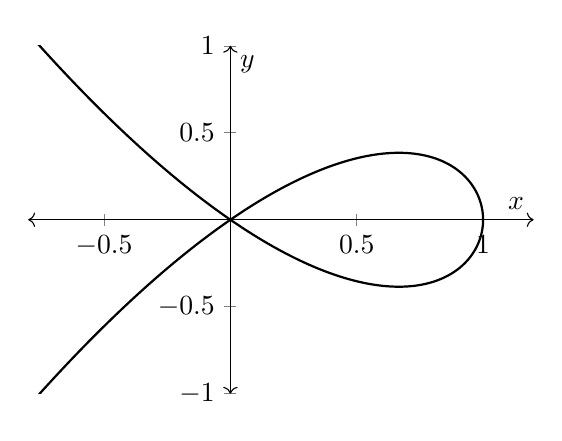
\begin{tikzpicture}
				\begin{axis}[
					height=6cm,
					width=8cm,
					xmin=-.8,xmax=1.2,
					ymin= -1,ymax=1,
					]
					\addplot [domain=-2:2,samples=1000, thick]({1-x^2},{x*(1-x^2)}); 
				\end{axis}
			\end{tikzpicture}
		\end{center}
		Then $M$ is not a $1$-dimensional topological manifold.\\
		\tbf{Hint:} connected components
	\end{ex}

	\begin{proof}
		Suppose that $M$ is a $1$-dimensional manifold. Set $p = (0,0)$. Then there exists $(U, \phi) \in X(M)$ such that $p \in U$. Since $\phi(U)$ is open (in $\R$ or $\H$), there exists a $B \subset \phi(U)$ such that $B$ is open (in $\R$ or $\H$), $B$ is connected and $\phi(p) \in B$. Set $V = \phi^{-1}(B)$, $V' = V \setminus \{p\}$ and $B' = B \setminus \{\phi(p)\}$. Then $\phi: V \rightarrow B$ and $\phi': V' \rightarrow B'$ are homeomorphisms. Since $B$ is open (in $\R$ or $\H$) and connected, $B'$ has at most two connected components. Then $V'$ This is a contradiction since $V'$ has four connected components and $B'$ and $V'$ are homeomorphic. 
	\end{proof}



	\begin{ex} \tbf{Topological Manifold Chart Lemma:} \\
	Let $M$ be a set, $\Gam$ an index set and for each $\al \in \Gam$, $U_{\al} \subset M$ and $\phi_{\al}: U_{\al} \rightarrow \H^n$. Suppose that 
	\begin{itemize}
		\item for each $\al \in \Gam$, $\phi_{\al}(U_{\al}) \in \MT_{\H^n}$ 
		\item for each $\al, \be \in \Gam$, $\phi_{\al}(U_{\al} \cap U_{\be}) \in \MT_{\H^n}$
		\item for each $\al \in \Gam$, $\phi_{\al}: U_{\al} \rightarrow \phi_{\al}(U_{\al})$ is a bijection
		\item for each $\al, \be \in \Gam$, $\phi_{\be}|_{U_{\al} \cap U_{\be}} \circ (\phi_{\al}|_{U_{\al} \cap U_{\be}})^{-1}: \phi_{\al}(U_{\al} \cap U_{\be}) \rightarrow \phi_{\be}(U_{\al} \cap U_{\be})$ is continuous
		\item there exists $\Gam' \subset \Gam$ such that $\Gam'$ is countable and $M \subset \bigcup\limits_{\al \in \Gam'} U_{\al}$
		\item for each $p,q \in M$, there exists $\al \in \Gam$ such that $p,q \in U_{\al}$ or there exist $\al,\be \in \Gam$ such that $p \in U_{\al}$, $q \in U_{\be}$ and $U_{\al} \cap U_{\be} = \varnothing$
	\end{itemize}
	Define 
	\begin{itemize}
		\item $\MB = \{\phi_{\al}^{-1}(V): V \in \MT_{\H^n} \text{ and $\al \in \Gam$} \}$
		\item $\MT_M = \tau(\MB)$
	\end{itemize}
	Then  
	\begin{enumerate}
		\item $\MB$ is a basis for $\MT_M$ \\
		\tbf{Hint:} For $B_1, B_2 \subset \H^n$, $\phi_{\al_1}^{-1}(B_1) \cap \phi_{\al_2}^{-1}(B_2) = \phi_{\al_1}^{-1}( B_1 \cap [\phi_{\al_1}|_{U_{\al_1} \cap U_{\al_2}} \circ (\phi_{\al_2}|_{U_{\al_1} \cap U_{\al_2}})^{-1}(B_2)])$
		\item $(M, \MT_M)$ is an $n$-dimensional topological manifold
		\item $\MT_M$ is the unique topology $\MT$ on $M$ such that $(U_{\al}, \phi_{\al})_{\al \in \Gam} \subset X^n(M, \MT)$
	\end{enumerate}
\end{ex}

\begin{proof} \
	\begin{enumerate}
		\item \begin{itemize}
			\item By assumption, $M \subset \bigcup\limits_{\al \in \Gam} U_{\al}$
			\item Let $A_1, A_2 \in \MB$ and $p \in A_1 \cap A_2$. By definition, there exist $\al_1, \al_2 \in \Gam$ and $B_1, B_2 \subset \H^n$ such that $B_1$, $B_2$ are open in $\H^n$ and 
			\begin{align*}
				A_1 & = \phi_{\al_1}^{-1}(B_1)  & A_2 & = \phi_{\al_2}^{-1}(B_2) \\
				& \subset U_{\al_1}         &     & \subset U_{\al_2}
			\end{align*}
			Set $\psi_1 = \phi_{\al_1}|_{U_{\al_1} \cap U_{\al_2}}$ and $\psi_2 = \phi_{\al_2}|_{U_{\al_1} \cap U_{\al_2}}$. We note that  
			\begin{align*}
				\psi_1^{-1}(B_1) & = U_{\al_2} \cap \phi_{\al_1}^{-1}(B_1) &  \psi_2^{-1}(B_2) & = U_{\al_1} \cap \phi_{\al_2}^{-1}(B_2) \\
				& = U_{\al_2} \cap A_1                    &                   & = U_{\al_1} \cap A_2 \\
				& \subset U_{\al_1} \cap U_{\al_2}        &                   & \subset U_{\al_1} \cap U_{\al_2}
			\end{align*}
			Let $q \in \phi_{\al_1}^{-1}(B_1 \cap [\psi_1 \circ \psi_2^{-1}(B_2)])$. Then $\phi_{\al_1}(q) \in B_1 \cap [\psi_1 \circ \psi_2^{-1}(B_2)]$. Hence $\phi_{\al_1}(q) \in B_1$ and $\phi_{\al_1}(q) \in \psi_1 \circ \psi_2^{-1}(B_2)$. This implies that  
			\begin{align*}
				q 
				& \in \phi_{\al_1}^{-1}(B_1) \\
				& = A_1
			\end{align*}
			and since $\psi_2^{-1}(B_2) \subset U_{\al_1} \cap U_{\al_2}$ and $\phi_{\al_1}: U_{\al_1} \rightarrow \phi_{\al_1}(U_{\al_1})$ is a bijection, we have that
			\begin{align*}
				q 
				& \in \phi_{\al_1}^{-1}(\psi_1 \circ \psi_2^{-1}(B_2)) \\
				& = \psi_2^{-1}(B_2) \\
				& = U_{\al_1} \cap A_2 
			\end{align*} 
			Thus 
			\begin{align*}
				q 
				& \in A_1 \cap (U_{\al_1} \cap A_2) \\
				& = A_1 \cap A_2
			\end{align*}
			Since $q \in \phi_{\al_1}^{-1}(B_1 \cap [\psi_1 \circ \psi_2^{-1}(B_2)])$ is arbitrary, we have that $\phi_{\al_1}^{-1}(B_1 \cap [\psi_1 \circ \psi_2^{-1}(B_2)]) \subset A_1 \cap A_2$. \\
			Conversely, let  
			\begin{align*}
				q 
				& \in A_1 \cap A_2 \\ 
				& = \phi_{\al_1}^{-1}(B_1) \cap \phi_{\al_2}^{-1}(B_2)
			\end{align*}
			Then $\phi_{\al_1}(q) \in B_1$ and $\phi_{\al_2}(q) \in B_2$. Since $A_1 \cap A_2 \subset U_{\al_1} \cap U_{\al_2}$, we have that 
			\begin{align*}
				\psi_2(q)
				& = \phi_{\al_2}(q) \\
				& \in B_2
			\end{align*}
			which implies that $q \in \psi_2^{-1}(B_2)$. Therefore 
			\begin{align*}
				\phi_{\al_1}(q)
				& = \psi_1(q) \\
				& \in \psi_1 ( \psi_2^{-1}(B_2)) \\
				& =  \psi_1 \circ \psi_2^{-1}(B_2) 
			\end{align*}
			Hence $\phi_{\al_1}(q) \in B_1 \cap [\psi_1 \circ \psi_2^{-1}(B_2)]$. This implies that $q \in \phi_{\al_1}^{-1}( B_1 \cap [\psi_1 \circ \psi_2^{-1}(B_2)])$. Since $q \in A_1 \cap A_2$ is arbitrary, we have that $A_1 \cap A_2 \subset \phi_{\al_1}^{-1}( B_1 \cap [\psi_1 \circ \psi_2^{-1}(B_2)])$. Thus 
			\begin{align*}
				A_1 \cap A_2 
				& = \phi_{\al_1}^{-1}( B_1 \cap [\psi_1 \circ \psi_2^{-1}(B_2)]) \\
				& \in \MB
			\end{align*}
			Thus $\MB$ is a basis for $\MT_M$.
		\end{itemize}
		\item 
		\begin{enumerate}
			\item \tbf{(locally Euclidean of dimension $n$):}\\
			Let $\al \in \Gam$. By definition, for each $B \subset \MT_{\H^n}$, 
			\begin{align*}
				\phi_{\al}^{-1}(B) 
				& \in \MB \\
				& \subset \MT_M
			\end{align*}
			Hence $\phi_{\al}$ is continuous. \\
			Let $A \in \MT_{U_{\al}}$. Then there exists $U \subset \MT_M$ such that $A = U \cap U_{\al}$. Since $\MB$ is a basis for $\MT_M$, there exists $\Gam' \subset \Gam$, $(V_{\be})_{\be \in \Gam'} \subset \MT_{\H^n}$ such that $U = \bigcup_{ \be \in \Gam'} \phi_{\be}^{-1}(V_{\be})$. Thus 
			\begin{align*}
				A
				& = U \cap U_{\al} \\
				& = \bigg[\bigcup_{\be \in \Gam'} \phi_{\be}^{-1}(V_{\be}) \bigg] \cap U_{\al} \\ 
				& = \bigcup_{\be \in \Gam'} [\phi_{\be}^{-1}(V_{\be}) \cap U_{\al}] \\
			\end{align*} 
			Let $\be \in \Gam'$. Since $\phi_{\al}(U_{\al} \cap U_{\be}) \subset \phi_{\al}(U_{\al})$ and $\phi_{\al}(U_{\al} \cap U_{\be}) \in \MT_{\H^n}$, we have that
			\begin{align*}
				\phi_{\al}(U_{\al} \cap U_{\be})
				& = \phi_{\al}(U_{\al}) \cap \phi_{\al}(U_{\al} \cap U_{\be}) \\
				& \in \MT_{\phi_{\al}(U_{\al})}
			\end{align*}
			Therefore $\MT_{\phi_{\al}(U_{\al} \cap U_{\be})} \subset \MT_{\phi_{\al}(U_{\al})}$. Since $(\phi_{\be}|_{U_{\al} \cap U_{\be}}) \circ (\phi_{\al}|_{U_{\al} \cap U_{\be}})^{-1}: \phi_{\al}(U_{\al} \cap U_{\be}) \rightarrow \phi_{\be}(U_{\al} \cap U_{\be})$ is continuous, we have that $(\phi_{\be}|_{U_{\al} \cap U_{\be}}) \circ (\phi_{\al}|_{U_{\al} \cap U_{\be}})^{-1}: \phi_{\al}(U_{\al} \cap U_{\be}) \rightarrow \H^n$
			is continuous and therefore 
			\begin{align*}
				[(\phi_{\be}|_{U_{\al} \cap U_{\be}}) \circ (\phi_{\al}|_{U_{\al} \cap U_{\be}})^{-1}]^{-1}(V_{\be}) 
				& \in \MT_{\phi_{\al}(U_{\al} \cap U_{\be})} \\
				& \subset \MT_{\phi_{\al}(U_{\al})}
			\end{align*} 
			Since $\be \in \Gam'$ is arbitrary, we have that
			\begin{align*}
				\phi_{\al}(A)
				& = \phi_{\al} \bigg( \bigcup_{\be \in \Gam'} [\phi_{\be}^{-1}(V_{\be}) \cap U_{\al}] \bigg) \\
				& = \bigcup_{\be \in \Gam'} \phi_{\al}(\phi_{\be}^{-1}(V_{\be}) \cap U_{\al}) \\
				& =  \bigcup_{\be \in \Gam'} (\phi_{\al}|_{U_{\al} \cap U_{\be}}) \circ (\phi_{\be}|_{U_{\al} \cap U_{\be}})^{-1}(V_{\be}) \\
				& =  \bigcup_{\be \in \Gam'} [(\phi_{\be}|_{U_{\al} \cap U_{\be}}) \circ (\phi_{\al}|_{U_{\al} \cap U_{\be}})^{-1}]^{-1}(V_{\be}) \\
				& \in \MT_{\phi_{\al}(U_{\al})}
			\end{align*} 
			Since $A \in \MT_{U_{\al}}$ is arbitrary, $\phi_{\al}^{-1}: \phi_{\al}(U_{\al}) \rightarrow U_{\al}$ is continuous. Hence $\phi_{\al}: U_{\al} \rightarrow \phi_{\al}(U_{\al})$ is a homeomorphism and $(U_{\al}, \phi_{\al}) \in X^n(M)$. Since $M = \bigcup\limits_{\al \in \Gam} U_{\al}$, we have that $M$ is locally Euclidean of dimension $n$.
			\item \tbf{(Hausdorff):} \\
			Let $p, q \in M$. Suppose that $p \neq q$. Then there exists $\al \in \Gam$ such that $p,q \in U_{\al}$ or there exist $\al, \be \in \Gam$ such that $p \in U_{\al}$, $q \in U_{\be}$ and $U_{\al} \cap U_{\be} = \varnothing$.
			\begin{itemize}
				\item Suppose that there exists $\al \in \Gam$ such that $p,q \in U_{\al}$. Since $p \neq q$, $\phi_{\al}(p) \neq \phi_{\al}(q)$. Since $\H^n$ is Hausdorff, there exist $V_p , V_q \subset \phi(U_{\al})$ such that $V_p$ and $V_q$ are open in $\H^n$, $p \in V_p$, $q \in V_q$ and $V_p \cap V_q = \varnothing$. Set $U_p = \phi_{\al}^{-1}(V_p)$ and $U_q = \phi_{\al}^{-1}V_q$. Then $U_p, U_q$ are open, $p \in U_p$, $q \in U_q$ and $U_q \cap U_p = \varnothing$.
				\item Suppose that there exist $\al, \be \in \Gam$ such that $p \in U_{\al}$, $q \in U_{\be}$ and $U_{\al} \cap U_{\be} = \varnothing$. Set $U_p = U_{\al}$ and $U_q = U_{\be}$. Then $U_p, U_q$ are open, $p \in U_p$, $q \in U_q$ and $U_q \cap U_p = \varnothing$.
			\end{itemize}
			Thus for each $p, q \in M$ there exist $U_p, U_q \subset M$ such that $U_p, U_q$ are open, $p \in U_p$, $q \in U_q$ and $U_q \cap U_p = \varnothing$. Hence 
			\item \tbf{(second-countable):} \\
			By assumption, there exists $\Gam' \subset \Gam$ such that $\Gam'$ is countable and $M \subset \bigcup\limits_{\al \in \Gam'} U_{\al}$. Let $\al \in \Gam'$. Since $\phi_{\al}(U_{\al}) \in \MT_{\H^n}$ and $\H^n$ is second-countable, we have that $\phi_{\al}(U_{\al})$ is second-countable. Since $\phi_{\al}: U_{\al} \rightarrow \phi_{\al}(U_{\al})$ is a homeomorphism, we have that $U_{\al}$ is second-countable. Since $M = \bigcup\limits_{\al \in \Gam'} U_{\al}$, an exercise in topology \tcb{cite} implies that $M$ is second-countable.
		\end{enumerate} 
	\item Let $\MT$ be a topology on $M$. Suppose that $(U_{\al}, \phi_{\al})_{\al \in \Gam} \subset X^n(M, \MT)$. Then for each $\al \in \Gam$, $U_{\al} \in \MT$ and $\phi_{\al}: U_{\al} \rightarrow \phi_{\al}(U_{\al})$ is a $(\MT \cap U_{\al}, \MT_{\H^n} \cap \phi_{\al}(U_{\al}))$-homeomorphism. \\ 
	Let $U \in \MB$. By definition, there exists $\al \in \Gam$ and $V \in \MT_{\H^n}$ such that $U = \phi_{\al}^{-1}(V)$. Since $U_{\al} \in \MT$, we have that $\MT \cap U_{\al} \subset \MT$. Since $V \cap \phi_{\al}(U_{\al}) \in \MT_{\H^n} \cap \phi_{\al}(U_{\al})$, and $\phi_{\al}$ is a  $(\MT \cap U_{\al}, \MT_{\H^n} \cap \phi_{\al}(U_{\al}))$-homeomorphism, we have that
	\begin{align*}
		U
		& = \phi_{\al}^{-1}(V) \\
		& = \phi_{\al}^{-1}(V \cap \phi_{\al}(U_{\al})) \\
		& \in \MT \cap U_{\al} \\
		& \subset \MT 
	\end{align*}
	Since $U \in \MB$ is arbitrary, $\MB \subset \MT$. Therefore 
	\begin{align*}
		\MT_M 
		& = \tau(\MB) \\
		& \subset \tau(\MT) \\
		& = \MT
	\end{align*}
	Conversely, Let $U \in \MT$ and $\al \in \Gam$. Then $U \cap U_{\al} \in \MT \cap U_{\al}$. Since $\phi_{\al}:U_{\al} \rightarrow \phi_{\al}(U_{\al})$ is a $(\MT \cap U_{\al}, \MT_{\H^n} \cap \phi_{\al}(U_{\al}))$-homeomorphism, we have that $\phi_{\al}(U \cap U_{\al}) \in \MT_{\H^n} \cap \phi_{\al}(U_{\al})$. Since $U_{\al} \in \MT_M$, $\MT_M \cap U_{\al} \subset \MT_M$. Since $\phi_{\al}:U_{\al} \rightarrow \phi_{\al}(U_{\al})$ is a $(\MT_M \cap U_{\al}, \MT_{\H^n} \cap \phi_{\al}(U_{\al}))$-homeomorphism, we have that 
	\begin{align*}
		U \cap U_{\al}
		& = \phi_{\al}^{-1}( \phi_{\al}(U \cap U_{\al})) \\
		& \in \MT_M \cap U_{\al} \\
		& \subset \MT_M 
	\end{align*}
	Then 
	\begin{align*}
		U
		& = U \cap M \\
		& = U \cap \bigg(\bigcup_{\al \in \Gam} U_{\al} \bigg) \\
		& = \bigcup_{\al \in \Gam} (U \cap U_{\al}) \\
		& \in \MT_M 
	\end{align*}
	Since $U \in \MT$ is arbitrary, $\MT \subset \MT_M$. Thus $\MT = \MT_M$.
	\end{enumerate}
\end{proof}

\begin{ex}
	Let $M$ be a set, $\Gam$ an index set and for each $\al \in \Gam$, $U_{\al} \subset M$ and $\phi_{\al}: U_{\al} \rightarrow \H^n$. Suppose that 
	\begin{itemize}
		\item for each $\al \in \Gam$, $\phi_{\al}(U_{\al}) \in \MT_{\H^n}$ 
		\item for each $\al, \be \in \Gam$, $\phi_{\al}(U_{\al} \cap U_{\be}) \in \MT_{\H^n}$
		\item for each $\al \in \Gam$, $\phi_{\al}: U_{\al} \rightarrow \phi_{\al}(U_{\al})$ is a bijection
		\item for each $\al, \be \in \Gam$, $\phi_{\be}|_{U_{\al} \cap U_{\be}} \circ (\phi_{\al}|_{U_{\al} \cap U_{\be}})^{-1}: \phi_{\al}(U_{\al} \cap U_{\be}) \rightarrow \phi_{\be}(U_{\al} \cap U_{\be})$ is continuous
		\item there exists $\Gam' \subset \Gam$ such that $\Gam'$ is countable and $M \subset \bigcup\limits_{\al \in \Gam'} U_{\al}$
		\item for each $p,q \in M$, there exists $\al \in \Gam$ such that $p,q \in U_{\al}$ or there exist $\al,\be \in \Gam$ such that $p \in U_{\al}$, $q \in U_{\be}$ and $U_{\al} \cap U_{\be} = \varnothing$
	\end{itemize}
	Then there exists a unique topology $\MT_M$ on $M$ such that $(M, \MT_M)$ is an $n$-dimensional topological manifold and $(U_{\al}, \phi_{\al})_{\al \in \Gam} \subset X^n(M, \MT_M)$.
\end{ex}

	\begin{proof}
		Immediate by previous exercise. 
	\end{proof}






	
	
	
	
	
	
	
	
	
	
	
	
	\newpage
	\section{Smooth Manifolds}

	\begin{defn}
		Let $M$ be an $n$-dimensional topological manifold and $(U, \phi), (V, \psi) \in X(M)$. Then $(U, \phi)$ and $(V, \psi)$ are said to be \tbf{smoothly compatible} if $$\psi|_{U \cap V} \circ (\phi|_{U \cap V})^{-1}: \phi(U \cap V) \rightarrow \psi (U \cap V) \text{ is a diffeomorphism}$$ 
	\end{defn}

	\begin{defn} Let $M$ be an $n$-dimensional topological manifold.
		\begin{itemize}
			\item Let $\MA \subset X(M)$. Then $\MA$ is said to be an \tbf{atlas on $M$} if  $M \subset \bigcup\limits_{(U,\phi) \in \MA} U$.
			\item Let $\MA$ be an atlas on $M$. Then $\MA$ is said to be \tbf{smooth} if for each $(U, \phi), (V, \psi) \in \MA$, $(U,\phi)$ and $(V,\psi)$ are smoothly compatible.
			\item Let $\MA$ be a smooth atlas on $M$. Then $\MA$ is said to be \tbf{maximal} if for each smooth atlas $\MB$ on $M$, $\MA \subset \MB$ implies that $\MA = \MB$. A maximal smooth atlas on $M$ is called a \tbf{smooth structure on $M$}.
			\item Let $\MA$ be an atlas on $M$. Then $(M, \MA)$ is said to be an \tbf{$n$-dimensional smooth manifold} if $\MA$ is a smooth structure on $M$. 
		\end{itemize}
	\end{defn}

	\begin{ex}
		Let $M$ be an $n$-dimensional topological manifold and $\MB$ a smooth atlas on $M$. Then there exists a unique smooth structure $\MA$ on $M$ such that $\MB \subset \MA$.
	\end{ex}

	\begin{proof}
		Define 
		$$\MA = \{(U, \phi) \in X(M): \text{ for each $(V, \psi) \in \MB$,  $(U, \phi)$ and $(V, \psi) $ are smoothly compatible}\}$$ 
		Clearly $\MB \subset \MA$. Let $(U, \phi)$ and $(V, \psi) \in \MA$. Define $F: \phi(U \cap V) \rightarrow \psi (U \cap V)$ by 
		$$F = \psi|_{U \cap V} \circ (\phi|_{U \cap V})^{-1}$$
		Let $q \in \phi(U \cap V)$. Set $p = \phi^{-1}(q)$. Since $p \in U \cap V \subset M$, there exists $(W, \chi) \in \MB$ such that $p \in W$. By definition of $\MA$, $\psi|_{W \cap V} \circ (\chi|_{W \cap V})^{-1} : \chi(W \cap V) \rightarrow \psi(W \cap V)$ and $ \chi|_{U \cap W} \circ (\phi|_{U \cap W})^{-1} : \phi(U \cap W) \rightarrow \chi(U \cap W)$ are diffeomorphisms. Set $N = U \cap W \cap V$. Then $q \in \phi(N) \subset \phi(U \cap V)$ and 
		\begin{align*}
			F|_{\phi(N)}
			& = \psi|_{N} \circ (\phi|_{N})^{-1} \\
			& = [\psi|_{N} \circ (\chi|_{N})^{-1}] \circ [\chi|_{N} \circ (\phi|_{N})^{-1}]
		\end{align*}
		is a diffeomorphism. 
		Thus, for each $q \in \phi(U \cap V)$, there exists $N' \subset \phi(U \cap V)$ such that $F|_{N'}$ is a diffeomorphism. Hence $F$ is a diffeomorphism and $(U, \phi)$, $(V, \psi)$ are smoothly compatible. Therefore $\MA$ is a smooth atlas.\\
		To see that $\MA$ is maximal, let $\MB'$ be a smooth atlas on $M$. Suppose that $\MA \subset \MB'$ and let $(U, \phi) \in \MB'$. By definition, for each chart $(V, \psi) \in \MB'$, $(U, \phi)$ and $(V, \psi)$ are smoothly compatible. Since $\MB \subset \MA \subset \MB'$, we have that $(U, \phi) \in \MA$. So $\MA = \MB'$ and $\MA$ is a maximal smooth atlas on $M$.
	\end{proof}

	\begin{ex}
		Let $(M, \MA)$ be an $n$-dimensional smooth manifold, $(U, \phi) \in \MA$ and $U' \subset U$. If $U'$ is open, then $(U', \phi|_{U'}) \in \MA$. 
	\end{ex}

	\begin{proof}
	Set $\phi' = \phi|_{U'}$. A previous exercise implies that $(U', \phi') \in X(U)$. Define $\MB = \MA \cup \{(U', \phi')\}$. Let $(V, \psi) \in \MB$. If $(V, \psi) = (U', \phi')$, then 
	$$\phi' \circ \psi^{-1} = \id_{U'}$$
	which is a diffeomorphism. Thus $(U', \phi')$, $(V, \psi)$ are smoothly compatible. Suppose that $(V, \psi) \in \MA$. Since $\MA$ is smooth, $\psi|_{U \cap V} \circ (\phi|_{U \cap V})^{-1}: \phi(U \cap V) \rightarrow \psi(U \cap V)$ is a diffeomorphism. Therefore $\psi|_{U' \cap V} \circ (\phi'|_{U' \cap V})^{-1}: \phi'(U' \cap V) \rightarrow \psi(U' \cap V)$ is a diffeomorphism and $(U', \phi')$, $(V, \psi)$ are smoothly compatible. Since $(V, \psi) \in \MA$ is arbitrary, $\MB$ is smooth. Since $\MA$ is maximal and $\MA \subset \MB$, we have that $\MA = \MB$ and $(U', \phi') \in \MA$.
	\end{proof}

	\begin{ex}
		Let $(M, \MA)$ be a $n$-dimensional smooth manifold and $U \subset M$ open. Set $\MB = \{(V, \psi) \in \MA: V \subset U\}$. Then $\MB$ is a smooth atlas on $U$.
	\end{ex}

	\begin{proof}\
		\begin{itemize}
			\item Some previous exercises imply that $U$ is an $n$-dimensional topological manifold and $X(U) = \{(V, \psi) \in X(M): V \subset U\}$. Since 
			\begin{align*}
				\MB 
				& \subset \MA \\
				& \subset X(M)
			\end{align*}
			we have that $\MB \subset X(U)$. Let $p \in U$. Then there exists $(V, \psi) \in \MA$ such that $p \in V$. Set $V' = U \cap V$ and $\psi' = \psi|_{V'}$. The previous exercise implies that $(V', \psi') \in \MA$. By definition, $(V', \psi') \in \MB$. Since $p \in U$ is arbitrary, we have that for each $p \in U$, there exists $(V', \psi') \in \MB$ such that $p \in V'$. Hence $\MB$ is an atlas on $U$. 
			\item Let $(V_1, \psi_1), (V_2, \psi_2) \in \MB$. Then $(V_1, \psi_1), (V_2, \psi_2) \in \MA$. Since $\MA$ is smooth, $(V_1, \psi_1)$ and $(V_2, \psi_2)$ are smoothly compatible. Since $(V_1, \psi_1), (V_2, \psi_2) \in \MB$ are arbitrary, $\MB$ is smooth.
		\end{itemize}
 	\end{proof}
 
 	\begin{defn} \tbf{Smooth Open Submanifold:} \\
 		Let $(M, \MA)$ be an $n$-dimensional smooth manifold and $U \subset M$ open. A previous exercise implies that $U$ is an $n$-dimensional topological manifold. We define $\MA|_{U} \subset X(U)$ to be the unique smooth structure on $U$ such that $\{(V, \psi) \in \MA: V \subset U\} \subset \MA|_{\MU}$. Then $(U, \MA|_{U})$ is said to be a \tbf{smooth open submanifold of $(M, \MA)$}.
 	\end{defn}
 
 	\begin{ex}
 		Let $\pi: \p \H^n \rightarrow \R^{n-1}$ be the projection map given by $\pi(x_1, \ldots, x_{n-1}, 0) = (x_1, \ldots, x_{n-1})$. Then $\pi$ is a diffeomorphism. 
 	\end{ex}
 
 	\begin{proof}
 		Define projection map $\pi': \R^n \rightarrow \R^{n-1}$ by $\pi'(x_1, \ldots, x_{n-1}, x_n) = (x_1, \ldots, x_{n-1})$. Then $\R^n$ is an open neighborhood of $\p H^n$, $\pi'|_{\p H^n} = \pi$ and $\pi'$ is smooth. Then by definition, $\pi$ is smooth. Clearly, $\pi^{-1}$ is smooth. So $\pi$ is a diffeomorphism.
 	\end{proof}

	\begin{defn} 
		Let $(M, \MA)$ be a $n$-dimensional smooth manifold and $\pi: \p \H^n \rightarrow \R^{n-1}$ the projection map. Recall that for $(U, \phi) \in X^n_{\p}(M)$, the $(n-1)$-coordinate chart $(\bar{U}, \bar{\phi}) \in X^{n-1}_{\Int}(\p M)$ is defined by $\bar{U} = U \cap \p M$ and $\bar{\phi} = \pi|_{\phi(\bar{U})} \circ \phi|_{\bar{U}}$. \\
		We define 
		$$\ol{\MA} = \{(\bar{U}, \bar{\phi}): (U, \phi) \in \MA \cap X^n_{\p}(M) \}$$
	\end{defn}
	
	\begin{ex}
		Let $(M, \MA)$ be a $n$-dimensional smooth manifold. Then $\ol{\MA}$ is a smooth atlas on $\p M$.
	\end{ex}
	
	\begin{proof}\
		\begin{itemize}
			\item A previous exercise implies that $\p M$ is an $(n-1)$-dimensional topological manifold. Let $p \in \partial M$. Then there exists $(U, \phi) \in \MA$ such that $p \in U$. Since $\MA \subset X^n(M)$ and $p \in \p M$, we have that $p \in \bar{U}$ and a previous exercise implies that $(U, \phi) \in X^n_{\p}(M)$. By definition of $\ol{\MA}$, $(\bar{U}, \bar{\phi}) \in \ol{\MA}$. Since $p \in \p M$ is arbitrary, $\ol{\MA}$ is an atlas on $\p M$. 
			
			
			\item Let $(\bar{U}, \bar{\phi})$, $(\bar{V}, \bar{\psi}) \in \ol{\MA}$. Since $(U, \phi)$ and $(V, \psi)$ are smoothly compatible, $\psi|_{U \cap V} \circ (\phi|_{U \cap V})^{-1}$ is a diffeomorphism. Thus $\psi|_{\bar{U} \cap \bar{V}} \circ (\phi|_{\bar{U} \cap \bar{V}})^{-1}$ is a diffeomorphism. Since $\pi|_{\phi(U \cap V)}$ and $\pi|_{\psi(U \cap V)}$ are diffeomorphisms, $\pi|_{\phi(\bar{U} \cap \bar{V})}$ and $\pi|_{\psi(\bar{U} \cap \bar{V})}$ are diffeomorphisms. Then 
			\begin{align*}
				\bar{\psi}|_{\bar{U} \cap \bar{V}} \circ (\bar{\phi}|_{\bar{U} \cap \bar{V}})^{-1}
				& = \bigg[ \pi|_{\psi(\bar{U} \cap \bar{V})} \circ \psi|_{\bar{U} \cap \bar{V}} \bigg] \circ \bigg[ (\phi|_{\bar{U} \cap \bar{V}})^{-1} \circ( \pi|_{\phi(\bar{U} \cap \bar{V})})^{-1} \bigg] \\
				& =\pi|_{\psi(\bar{U} \cap \bar{V})} \circ \bigg[ \psi|_{\bar{U} \cap \bar{V}} \circ (\phi|_{\bar{U} \cap \bar{V}})^{-1} \bigg] \circ (\pi|_{\phi(\bar{U} \cap \bar{V})})^{-1}
			\end{align*}
			is a diffeomorphism. Therefore $(\bar{U}, \bar{\phi})$ and $(\bar{V}, \bar{\psi})$ are smoothly compatible. Since $(\bar{U}, \bar{\phi}), (\bar{V}, \bar{\psi}) \in \ol{\MA}$ are arbitrary, $\MA$ is smooth.
		\end{itemize}
	\end{proof}

	\begin{defn}
		Let $(M, \MA)$ be a $n$-dimensional smooth manifold. We define $\MA|_{\p M}$ to be the unique smooth structure on $\p M$ such that $\ol{\MA} \subset \MA|_{\p M}$. We define the \tbf{smooth boundary submanifold of $M$} to be $(\p M, \MA|_{\p M})$.
	\end{defn}

	
	\begin{ex} \tbf{Smooth Manifold Chart Lemma:} \\
		Let $M$ be a set, $\Gam$ an index set and for each $\al \in \Gam$, $U_{\al} \subset M$ and $\phi_{\al}: U_{\al} \rightarrow \H^n$. Suppose that 
		\begin{enumerate}[label=(\alph*)]
			\item for each $\al \in \Gam$, $\phi_{\al}(U_{\al}) \in \MT_{\H^n}$
			\item for each $\al, \be \in \Gam$, $\phi_{\al}(U_{\al} \cap U_{\be}) \in \MT_{\H^n}$
			\item for each $\al \in \Gam$, $\phi_{\al}: U_{\al} \rightarrow \phi_{\al}(U_{\al})$ is a bijection
			\item for each $\al, \be \in \Gam$, $\phi_{\be}|_{U_{\al} \cap U_{\be}} \circ (\phi_{\al}|_{U_{\al} \cap U_{\be}})^{-1}: \phi_{\al}(U_{\al} \cap U_{\be}) \rightarrow \phi_{\be}(U_{\al} \cap U_{\be})$ is smooth
			\item there exists $\Gam' \subset \Gam$ such that $\Gam'$ is countable and $M \subset \bigcup\limits_{\al \in \Gam'} U_{\al}$
			\item for each $p,q \in M$, there exists $\al \in \Gam$ such that $p,q \in U_{\al}$ or there exist $\al,\be \in \Gam$ such that $p \in U_{\al}$, $q \in U_{\be}$ and $U_{\al} \cap U_{\be} = \varnothing$
		\end{enumerate}
		Then there exists a unique smooth structure $\MA_M$ on $M$ such that $(M, \MA_M)$ is an $n$-dimensional smooth manifold and $(U_{\al}, \phi_{\al})_{\al \in \Gam} \subset \MA_M$.
	\end{ex}

	\begin{proof}
		Define
		\begin{itemize}
			\item $\MB = \{\phi_{\al}^{-1}(V): \al \in \Gam \text{ and } V \in \MT_{\H^n}\}$ 
			\item $\MT_M = \tau(\MB)$ 
			\item $\MA' = \{(U_{\al}, \phi_{\al}) : \al \in \Gam\}$.
		\end{itemize}
		The topological manifold chart lemma implies that $(M, \MT_M)$ is an $n$-dimensional topological manifold and $\MA' \subset X^n(M, \MT_M)$. Since $M = \bigcup_{\al \in \Gam} U_{\al}$, $\MA'$ is an atlas on $M$. Since for each $\al, \be \in \Gam$, $\phi_{\be}|_{U_{\al} \cap U_{\be}} \circ (\phi_{\al}|_{U_{\al} \cap U_{\be}})^{-1}: \phi_{\al}(U_{\al} \cap U_{\be}) \rightarrow \phi_{\be}(U_{\al} \cap U_{\be})$ is smooth, we have that $\MA'$ is smooth. A previous exercise implies that there exists a unique smooth structure $\MA_M$ on $M$ such that $\MA' \subset \MA_M$. 
	\end{proof}
	
	
	
	
	
	
	
	
	
	
	
	

	
	
	
	
	
	
	
	
	
	
	
	
	
	
	
	
	\newpage 
	\section{Smooth Maps}	
	
	\begin{defn} \ld{42001}
		Let $(M, \MA)$ be a smooth manifold and $f: M \rightarrow \R$. Then $f$ is said to be smooth if for each coordinate chart $(U, \phi) \in \MA$, $f \circ \phi^{-1}: \phi(U) \rightarrow \R$ is smooth. The set of all smooth functions on $M$ is denoted $C^{\infty}(M)$. 
	\end{defn}

	\begin{ex} \ld{42002}
		Let $(M, \MA)$ be a smooth manifold. Then $C^{\infty}(M)$ is a vector space.
	\end{ex}

	\begin{proof}
		Let $f,g \in C^{\infty}(M)$, $\lam \in \R$ and $(U, \phi) \in \MA$. By assumption, $f \circ \phi^{-1}$ and $g \circ \phi^{-1}$ are smooth. Hence 
		$$(f + \lam g) \circ \phi^{-1} = f \circ \phi^{-1} + \lam g \circ \phi^{-1} $$
		is smooth. Since $(U, \phi) \in \MA$ is arbitrary, $f + \lam g \in C^{\infty}(M)$. Since $f,g \in C^{\infty}(M)$ and $\lam \in \R$ are arbitrary, $C^{\infty}(M)$ is a vector space.
	\end{proof}

	\begin{ex}
		Let $(M, \MA)$ be a smooth manifold, $\MB$ an atlas on $M$ and $f:M \rightarrow \R$. Suppose that $\MB \subset \MA$. Then $f$ is smooth iff for each $(U, \phi) \in \MB$, $f \circ \phi^{-1}: \phi(U) \rightarrow \R$ is smooth.
	\end{ex}

	\begin{proof}\
		\begin{itemize}
			\item ($\implies$): \\
			Suppose that $f$ is smooth. Let $(U, \phi) \in \MB$. Since $\MB \subset \MA$, $(U, \phi) \in \MA$. Since $f$ is smooth, $ f \circ \phi^{-1}$ is smooth. Since $(U, \phi) \in \MB$ is arbitrary, we have that for each $(U, \phi) \in \MB$, $f \circ \phi^{-1}$ is smooth.
			\item ($\impliedby$): \\
			Suppose that for each $(V, \psi) \in \MB$, $f \circ \psi^{-1}: \psi(V) \rightarrow \R$ is smooth. Let $(U, \phi) \in \MA$ and $q \in \phi(U)$. Set $p = \phi^{-1}(q)$. Since $\MB$ is an atlas, there exists $(V, \psi) \in \MB$ such that $p \in V$. Since $\MB \subset \MA$, $(V, \psi) \in \MA$. Set $W = U \cap V$ and $\tilde{\phi} = \phi|_W$ and $\tilde{\psi} = \psi|_W$. We note that $\phi(W) \in \MN_q$ and $\phi(W)$ is open. An exercise in the section on smooth manifolds implies that $(W, \tilde{\phi}), (W, \tilde{\psi}) \in \MA$. Therefore $\tilde{\psi} \circ \tilde{\phi}^{-1}: \phi(W) \rightarrow \psi(W)$ is smooth. By assumption, $f \circ \psi^{-1}: \psi(V) \rightarrow \R$ is smooth. This implies that $(f \circ \psi^{-1})|_{\psi(W)}: \psi(W) \rightarrow \R$ is smooth. Hence
			\begin{align*}
				(f \circ \phi^{-1})|_{\phi(W)}
				& = f \circ \tilde{\phi}^{-1} \\
				& = f \circ (\tilde{\psi}^{-1} \circ \tilde{\psi}) \circ \tilde{\phi}^{-1} \\
				& = (f \circ \tilde{\psi}^{-1}) \circ (\tilde{\psi} \circ \tilde{\phi}^{-1})
			\end{align*}
			is smooth. Since $q \in \phi(U)$ is arbitrary, for each $q \in \phi(U)$, there exists $A \in \MN_q$ such that $A$ is open and $(f \circ \phi^{-1})|_{A}:A \rightarrow \R$ is smooth. This implies that $f \circ \phi^{-1}: \phi(U) \rightarrow \R$ is smooth. Since $(U, \phi) \in \MA$ is arbitrary, $f$ is smooth.
		\end{itemize}
	\end{proof}
	
	\begin{ex}
	Let $(M, \MA)$ be a smooth manifold, $(U, \phi) \in \MA$ with $\phi = (x^1, \cdots, x^n)$, $p \in U$ and $f \in C^{\infty}(M)$. Then $f|_U \in C^{\infty}(U)$.
	\end{ex}
	
	\begin{proof}\
	Let 
	\end{proof}
	
	\begin{defn}
	Let $(M, \MA)$ be a smooth manifold, $(U, \phi) \in \MA$ with $\phi = (x^1, \cdots, x^n)$, $f \in C^{\infty}(U)$ and $i \in \{1, \cdots, n\}$. We define the \tbf{partial derivative of $f$ with respect to $x^i$}, denoted $$ \p f / \p x^i: U \rightarrow \R \hspace{.1cm} \text{ or } \hspace{.1cm} \p_{i} f: U \rightarrow \R$$ by 
	\begin{equation*}
	\frac{\p f}{\p x^i}(p) = {\frac{\p}{\p u^i}[f \circ \phi^{-1}] }( \phi(p)) 
	\end{equation*}
	or equivalently,
	\begin{equation*}
	\frac{\p f}{\p x^i} = \bigg({\frac{\p}{\p u^i}[f \circ \phi^{-1}] \bigg) \circ \phi }
	\end{equation*}
	\end{defn}
	
	\begin{ex}
	Let $(M, \MA)$ be a smooth manifold, $(U, \phi) \in \MA$ with $\phi = (x^1, \cdots, x^n)$, $f \in C^{\infty}(U)$ and $i \in \{1, \cdots, n\}$. Then $\p / \p x^i:  C^{\infty}(U) \rightarrow C^{\infty}(U)$ is linear.
	\end{ex}
	
	\begin{proof}
	\tbf{FINISH!!!}
	\end{proof}
	
	\begin{ex}
	Let $(M, \MA)$ be a smooth manifold, $(U, \phi) \in \MA$ with $\phi = (x^1, \cdots, x^n)$, $f \in C^{\infty}(U)$ and $i,j \in \{1, \cdots, n\}$. Then 
	$$\frac{\p}{\p x^i}\frac{\p}{\p x^j} f =  \bigg(\frac{\p}{\p u^i} \frac{\p}{\p u^j}[f \circ \phi^{-1}] \bigg) \circ \phi $$
	\end{ex}
	
	\begin{proof}
	
	\begin{align*}
	\frac{\p}{\p x^i}\frac{\p}{\p x^j} f 
	&=\frac{\p}{\p x^i} \bigg(\frac{\p}{\p x^j} f \bigg) \\
	&=\frac{\p}{\p x^i} \bigg( \bigg[\frac{\p}{\p u^j} [f \circ \phi^{-1}] \bigg] \circ \phi \bigg) \\
	&=  \bigg( \frac{\p}{\p u^i} \bigg[ \bigg( \bigg[\frac{\p}{\p u^j} [f \circ \phi^{-1}] \bigg] \circ \phi \bigg) \circ \phi^{-1} \bigg] \bigg) \circ \phi \\
	&= \bigg( \frac{\p}{\p u^i} \bigg[\frac{\p}{\p u^j} [f \circ \phi^{-1}] \bigg]  \bigg) \circ \phi \\
	&= \bigg( \frac{\p}{\p u^i} \frac{\p}{\p u^j} [f \circ \phi^{-1}]  \bigg) \circ \phi \\
	\end{align*}
	\end{proof}
	
	\begin{ex}
	Let $(M, \MA)$ be a smooth manifold, $(U, \phi) \in \MA$ with $\phi = (x^1, \cdots, x^n)$ and $i,j \in \{1, \cdots, n\}$. Then 
	\begin{equation*}
	\frac{\p}{\p x^i}\frac{\p}{\p x^j} =\frac{\p}{\p x^j}\frac{\p}{\p x^i}
	\end{equation*}
	\end{ex}
	
	\begin{proof}
	Let $f \in C^{\infty}(U)$. Since $f \circ \phi^{-1}$ is smooth, $$\frac{\p}{\p u^i} \frac{\p}{\p u^j} [f \circ \phi^{-1}] = \frac{\p}{\p u^j} \frac{\p}{\p u^i} [f \circ \phi^{-1}] $$
	The previous exercise implies that 
	
	\begin{align*}
	\frac{\p}{\p x^i}\frac{\p}{\p x^j}f 
	&= \bigg( \frac{\p}{\p u^i} \frac{\p}{\p u^j} [f \circ \phi^{-1}]  \bigg) \circ \phi \\
	&= \bigg( \frac{\p}{\p u^j} \frac{\p}{\p u^i} [f \circ \phi^{-1}]  \bigg) \circ \phi \\
	&=\frac{\p}{\p x^j}\frac{\p}{\p x^i}f 
	\end{align*}
	\end{proof}
	
	\begin{ex}
	Let $(M, \MA)$ be a smooth manifold, $(U, \phi) \in \MA$ with $\phi = (x^1, \cdots, x^n)$ and $f \in C^{\infty}(U)$. Then for each $\al \in \N_0^n$, $$\p^{\al} f = (\p^{\al}[ f \circ \phi^{-1}] ) \circ \phi$$
	\end{ex}	
	
	\begin{proof}
	The claim is clearly true when $|\al| =0$ or by definition if $|\al| = 1$. Let $n \in \N$ and suppose the claim is true for each $|\al| \in \{1, \ldots, n-1 \}$. Then there exists $i \in \{1, \ldots, n\}$ such that $\al_i \geq 1$. Hence 
	\begin{align*}
	\p^{\al}f 
	&= \p^{e^i} (\p^{\al - e^i} f) \\
	&= \p^{e^i} (\p^{\al - e^i}[ f \circ \phi^{-1}] \circ \phi) \\
	&= (\p^{e^i} [(\p^{\al - e^i}[ f \circ \phi^{-1}] \circ \phi) \circ \phi^{-1} ]) \circ \phi\\
	&= (\p^{e^i} [\p^{\al - e^i}[ f \circ \phi^{-1}]] )\circ \phi\\
	&= (\p^{\al}[ f \circ \phi^{-1}] )\circ \phi\\
	\end{align*}
	\end{proof}
	
	
	\begin{ex} \tbf{Taylor's Theorem:} \\
	Let $(M, \MA)$ be a smooth manifold, $(U, \phi) \in \MA$ with $\phi = (x^1, \ldots, x^n)$ and $\phi(U)$ convex, $p \in U$, $f \in C^{\infty}(U)$ and $T \in \N$. Then there exist $(g_{\al})_{|\al| = T+1} \subset C^{\infty}(U)$ such that
		$$f = \sum_{k=0}^{T} \bigg[\sum_{|\al| = k}(x - p)^{\al} \p^{\al} f (x_0) \bigg] + \sum_{|\al| = T+1}(x^i - x^i(p))^{\al} g_{\al}$$ and for each $|\al|= T+1$, $$g_{\al}(p) = \frac{1}{(T+1)!}\p^{\al} f(p)$$
	\end{ex}
	
	\begin{proof}
	Since $\phi(U)$ is open and convex and $f \circ \phi^{-1} \in C^{\infty}(\phi(U))$, Taylors thorem in section $2.1$ implies that there exist $(\tilde{g}_{\al})_{|\al| = T+1} \subset C^{\infty}(\phi(U))$ such that for each $q \in U$, 
	$$f \circ \phi^{-1} (\phi(q)) = \sum_{k=0}^{T} \bigg[\sum_{|\al| = k}(x^i(q) - x^i(p))^{\al} \p^{\al} [f \circ \phi^{-1}] (\phi(p)) \bigg] + \sum_{|\al| = T+1}(x^i(q) - x^i(p))^{\al} \tilde{g}_{\al}(\phi(q)) $$	
		and for each $|\al|= T+1$, 
		\begin{align*}
		\tilde{g}_{\al}(\phi(p)) 
		&= \frac{1}{(T+1)!}\p^{\al} [f \circ \phi^{-1}](\phi(p)) \\
		&= \frac{1}{(T+1)!}\p^{\al} f (p)
		\end{align*}
		For $|\al| = T+1$, set $g_{\al} = \tilde{g} \circ \phi$. Then 
		\begin{align*}
	f(q) 
	&= f \circ \phi^{-1} (\phi(q)) \\
	&= \sum_{k=0}^{T} \bigg[\sum_{|\al| = k}(x^i(q) - x^i(p))^{\al} \p^{\al} [f \circ \phi^{-1}] (\phi(p)) \bigg] + \sum_{|\al| = T+1}(x^i(q) - x^i(p))^{\al} \tilde{g}_{\al}(\phi(q)) \\
	&= \sum_{k=0}^{T} \bigg[\sum_{|\al| = k}(x^i(q) - x^i(p))^{\al} \p^{\al} f(p) \bigg] + \sum_{|\al| = T+1}(x^i(q) - x^i(p))^{\al} g_{\al}(q) \\
\end{align*}			
	\end{proof}

	\begin{defn}
		Let $(N, \MB)$ be a smooth manifold and $F: M \rightarrow N$. Then $F$ is said to be 
		\begin{itemize}
		\item \tbf{smooth} if for each $(U, \phi) \in \MA$ and $(V, \psi) \in \MB$, $$\psi \circ F \circ \phi^{-1}: \phi(U \cap F^{-1}(V)) \rightarrow \psi(F(U) \cap V)$$ is smooth 
		\item a \tbf{diffeomorphism} if $F$ is a bijection and $F,F^{-1}$ are smooth.
		\end{itemize}
	\end{defn}
	
	\begin{ex}
	Let $(M, \MA)$ and $(N, \MB)$ be smooth manifold and $F: M \rightarrow N$. If $F$ is smooth, then $F$ is continuous. 
	\end{ex}
	
	\begin{proof}
	Suppose that $F$ is smooth. Let $p \in M$. Choose $(U, \phi) \in \MA$ and $(V, \psi) \in \MB$ such that $p \in U$ and $F(p) \in V$. Put $\tU = U \cap F^{-1}(V)$ and $\tV = F(U) \cap V$. \\
	Define $\tphi: \tU \rightarrow \phi(\tU)$ and $\tpsi: \tV \rightarrow \psi(\tV)$ by $$\tphi = \phi|_{\tU}, \hspace{.2cm} \tphi = \psi|_{\tV}$$ Then $\tphi$ and $\tpsi$ are homeomorphisms, $p \in \tU$ and $F(\tU) \subset \tV$. Define $\tF: \phi(\tU) \rightarrow \psi(\tV) $ by $$ \tF = \tpsi \circ F \circ \tphi^{-1}$$  
	By definition, $\tF$ is smooth and therefore continuous. Since $\phi$ and $\psi$ are homeomorphisms and $F|_{\tU} = \tpsi^{-1} \circ \tF \circ \tphi$, we have that $F|_{\tU}$ is continuous. In particular, $F$ is continuous at $p$ and since $p \in M$ is arbitrary, $F$ is continuous.
	\end{proof}
	
	\begin{ex}
	Let $(M, \MA)$ and $(N, \MB)$ be smooth manifold and $F: M \rightarrow N$. If $F$ is a diffeomorphism, then $F$ is a homeomorphism. 
	\end{ex}	
	
	\begin{proof}
	Suppose that $F$ is a diffeomorphism. By definition, $F$ and  $F^{-1}$ are smooth. The previous exercise implies that $F$ and $F^{-1}$ are continuous. Hence $F$  is a homeomorphism. 
	\end{proof}
	
	\begin{ex}
		Let $(N, \MB)$ be a smooth manifold and $F: M \rightarrow N$ a diffeomorphism. Then for each $(U, \phi) \in \MA$, $(F(U), \phi \circ F^{-1}) \in \MB$.
	\end{ex}
	
	\begin{proof}
		Let $(V, \psi) \in \MB$. 
		\begin{enumerate}
		\item Since $\phi$ and $F^{-1}$ are homeomorphisms, $\phi \circ F^{-1}: F(U) \cap V \rightarrow \phi(U \cap F^{-1}(V))$ is a homeomorphism
		\item Since $F$ is a diffeomorphism, $$\phi \circ F^{-1} \circ \psi^{-1}: \psi(F(U) \cap V) \rightarrow \phi(U \cap F^{-1}(V))$$ and $$\psi \circ F \circ \phi^{-1}: \phi(F^{-1}(V) \cap U) \rightarrow \psi(V \cap F(U))$$ are smooth. 
		\end{enumerate}
		
		Therefore $(F(U), \phi \circ F^{-1})$ and $(V, \psi)$ are smoothly compatible. Since $\MB$ is maximal, $(F(U), \phi \circ F^{-1}) \in \MB$.
	\end{proof}


	\begin{defn}
		Let $(N, \MB)$ be a smooth  $n$-dimensional manifold, $F: M \rightarrow N$ smooth and $(V, \psi) \in \MB$ with $\psi = (y^1, \dots, y^n)$. For $i \in \{1, \dots, n\}$, We define the \tbf{$i$-th component of $F$ with respect to $(V, \psi)$},  denoted $F^i: V \rightarrow \R$, by $$F^i = y^i \circ F$$  
	\end{defn}

	











\newpage 
\section{Partitions of Unity}
	
	\begin{defn}
	Let $p \in M$, $U \in \MN_a$ open and $\rho \in C_c^{\infty}(M)$. Then $\rho$ is said to be a \tbf{bump function at p supported in $U$} if 
	\begin{enumerate}
	\item $\rho \geq 0$ 
	\item there exists $V \in \MN_p$ such that $V$ is open and $\rho|_V = 1$ 
	\item $\supp \rho \subset U$
	\end{enumerate}
	\end{defn}
	
	\begin{ex}
	Define $f:\R \rightarrow \R$ by 
	\[
	f(t) = 
	\begin{cases}
	e^{-\frac{1}{1-t^2}} & t \in (-1,1)\\
	0 &  t \not \in (-1,1)
	\end{cases}
	\]
	Then $f \in C_c^{\infty}(\R)$.
	\end{ex}
	
	\begin{proof}
	
	\end{proof}
	
	
















	\newpage
	\section{The Tangent Space}

%	\begin{defn}
%		Let $p \in M$. Define the relation $\sim_p$ on $C^{\infty}(M)$ by $f \sim_p g$ iff there exists $U \in \MN_p$ such that $U$ is open and $f|_U = g|_U$. Clearly $\sim_p$ is an equivalence relation on $C^{\infty}(M)$. We denote $C^{\infty}(M) / \sim_p$ by $C^{\infty}_p(M)$. For $f \in C^{\infty}(M)$, we define the \tbf{germ of $f$ at $p$} to be the equivalence class of $f$ under $\sim_p$. 
%	\end{defn}

	\begin{defn}
		Let $(U, \phi) \in \MA$ with $\phi = (x^1, \cdots, x^n)$ and $p \in U$. For $i \in \{1, \cdots, n\}$, define the partial derivative with respect to $x^i$ at $p$, denoted $$\frac{\p}{\p x^i} \bigg|_p: C^{\infty}(M) \rightarrow \R  \text{, or } \p_i|_p: C^{\infty}(M) \rightarrow \R $$ by $$ \frac{\p}{\p x^i} \bigg |_p  f =  \frac{\p f}{\p x^i}(p) $$
	\end{defn}

	\begin{ex}
		Let $(U, \phi) \in \MA$ with $\phi = (x^1, \cdots, x^n)$ and $p \in U$. Then for each $i,j \in \{1, \cdots, n\}$, we have that $${\frac{\p}{\p x^i}{x^j}}(p) = \del_{i,j}$$
	\end{ex}

	\begin{proof}
		Let $i,j \in \{1, \cdots, n\}$. Then 
		\begin{align*}
			\frac{\p}{\p x^i} \bigg|_p x^i 
			&=  \frac{\p}{\p u^i} \bigg|_{\phi(p)} x^i \circ \phi^{-1} \\
			&= \frac{\p}{\p u^i} \bigg|_{\phi(p)} u^i \circ \phi \circ \phi^{-1} \\
			&= \frac{\p}{\p u^i} \bigg|_{\phi(p)} u^i  \\
			&= \del_{i,j}
		\end{align*}
	\end{proof}

	\begin{ex} \tbf{Change of Coordinates:}\\
		Let $(U, \phi), (V, \psi) \in \MA$ with $\phi = (x^1, \cdots, x^n)$ and $\psi = (y^1, \cdots, y^n)$, $p \in U \cap V$ and $f \in C^{\infty}(M)$. Then for each $i \in \{1, \cdots, n\}$, 
		 $$\frac{\p}{\p y^i} \bigg|_p = \sum_{j =1}^n {\frac{\p}{\p x^j}{y^i}}(p) \frac{\p}{\p x^i} \bigg|_p    $$
	\end{ex}

	\begin{proof}
		Put $h = \phi \circ \psi^{-1}$ and write $h = (h_1, \cdots, h_n)$. Then $\phi = h \circ \psi$ and $\psi^{-1} = \phi^{-1} \circ h$. By definition and the chain rule, we have that 
		\begin{align*}
		\frac{\p}{\p y^i} \bigg|_p f 
			&= \frac{\p}{\p u^i} \bigg|_{\psi(p)} f \circ \psi^{-1} \\
			&= \frac{\p}{\p u^i} \bigg|_{\psi(p)} f \circ \phi^{-1} \circ h \\
			&= \sum_{j=1}^n \bigg(\frac{\p}{\p u^j} \bigg|_{h \circ \psi (p)} f \circ \phi^{-1} \bigg)  \bigg( \frac{\p}{\p u^i} \bigg|_{\psi(p)} h_j \bigg) \\
			&= \sum_{j=1}^n \bigg(\frac{\p}{\p u^j} \bigg|_{\phi (p)} f \circ \phi^{-1}  \bigg) \bigg( \frac{\p}{\p u^i} \bigg|_{\psi(p)} x^j \circ \psi^{-1} \bigg) \\
			&= \sum_{j=1}^n \bigg( \frac{\p}{\p x^i} \bigg|_p f \bigg)  \bigg(   \frac{\p}{\p y^i} \bigg|_p x^j  \bigg)\\
		\end{align*}
	\end{proof}

	\begin{defn}
		Let $p \in M$ and $v: C^{\infty}(M) \rightarrow \R$. Then $v$ is said to be \tbf{Leibnizian} if for each $f,g \in  C^{\infty}(M)$, $$v(fg) = v(f)g(p) + f(p)v(g)$$ and $v$ is said to be a \tbf{derivation at $p$} if for each $f, g \in C^{\infty}(M)$ and $a \in \R$,
		\begin{enumerate}
			\item $v$ is linear 
			\item $v$ is Leibnizian
		\end{enumerate}
		We define the \tbf{tangent space of $M$ at $p$}, denoted $T_pM$, by $$T_pM = \{ v: C^{\infty}(M) \rightarrow \R: v \text{ is a derivation at }p\}$$
	\end{defn}

	\begin{ex}
		Let $f \in C^{\infty}(M)$ and $v \in T_pM$. If $f$ is constant, then $vf = 0$.
	\end{ex}

	\begin{proof}
		Suppose that $f = 1$. Then $f^2 = f$ and $v(f^2) = 2v(f)$. So $v(f) = 2v(f)$ which implies that $v(f) = 0$. If $f \neq 1$, then there exists $c \in \R$ such that $f = c$. Since $v$ is linear, $v(f) = cv(1) = 0$.
	\end{proof}

	\begin{ex}
		Let $(U, \phi) \in \MA$ with $\phi = (x^1, \cdots, x^n)$ and $p \in U$. Then $$ \bigg \{\frac{\p}{\p x^1} \bigg|_p, \cdots, \frac{\p}{\p x^n} \bigg|_p \bigg \}$$ is a basis for $T_pM$ and $\dim T_pM = n$.
	\end{ex}

	\begin{proof}
		Clearly $\frac{\p}{\p x^1} \bigg|_p, \cdots, \frac{\p}{\p x^n} \bigg|_p \in T_pM$. Let $a_1, \cdots, a_n \in \R$. Suppose that $$v = \sum_{i=1}^n a_i \frac{\p}{\p x^i} \bigg |_p  = 0$$
		Then 
		\begin{align*}
			0
			&= v x^j \\
			&= \sum_{i=1}^n a_i \frac{\p}{\p x^i} \bigg |_p  x^j \\
			&= a_j
		\end{align*}
		Hence $\bigg \{\frac{\p}{\p x^1} \bigg|_p, \cdots, \frac{\p}{\p x^n} \bigg|_p \bigg \}$ is independent.\\
		Now, let $v \in T_pM$ and $f \in \C^{\infty}(M)$. By Taylor's theorem, there exist $g_1, \cdots g_n \in C_p^{\infty}(M)$ such that $$f = f(p) + \sum_{i=1}^n(x^i - x^i(p)) g_i$$ and for each $i \in \{1, \cdots, n\}$, $$g_i(p) = \frac{\p}{\p x^i} \bigg |_p  f $$ Then 
		\begin{align*}
			v(f)
			&= \sum_{i=1}^nv(x^i - x^i(p)) g_i(p) + \sum_{i=1}^n(x^i(p) - x^i(p)) v(g_i) \\
			&= \sum_{i=1}^nv(x^i)g_i(p) \\
			&= \sum_{i=1}^nv(x^i)\frac{\p}{\p x^i} \bigg |_p  f \\
			&= \bigg[ \sum_{i=1}^nv(x^i)\frac{\p}{\p x^i} \bigg |_p  \bigg] f
		\end{align*}
		So $$v = \sum_{i=1}^nv(x^i)\frac{\p}{\p x^i} \bigg |_p  $$ and $$v \in \spn \bigg \{\frac{\p}{\p x^1} \bigg|_p, \cdots, \frac{\p}{\p x^n} \bigg|_p \bigg \}$$
	\end{proof}



	\begin{defn}
		Let $(N, \MB)$ be a smooth manifold, $F: M \rightarrow N$ smooth and $p \in M$. We define the \tbf{differential of $F$ at $p$}, denoted $DF_p: T_pM \rightarrow T_{F(p)}N$, by $$\bigg[ DF_p(v) \bigg] (f) = v (f \circ F)$$  for $v \in T_pM$ and $f \in C^{\infty}(N)$.
	\end{defn}
	
	
	
	\begin{ex}
	Let $(N, \MB)$ be a smooth manifold, $F: M \rightarrow N$ smooth and $p \in M$. Then for each $v \in T_pM$, $DF_p(v)$ is a derivation.
	\end{ex}
	
	\begin{proof}
	Let $v \in T_pM$, $f,g \in C_{F(p)}^{\infty}(N)$ and $c \in \R$. Then 
	\begin{enumerate}
	\item 
	\begin{align*}
		DF_p(v)(f+cg) 
		&= v((f+cg) \circ F) \\
		&= v(f \circ F + c g \circ F) \\
		&= v(f \circ F) + cv(g \circ F) \\
		&= DF_p(v)(f) + c DF_p(v)(g)
	\end{align*}
	So $DF_p(v)$ is linear.
	\item 
	\begin{align*}
	DF_p(v)(fg) 
	&= v (fg \circ F) \\
	&= v((f \circ F)* (g \circ F)) \\
	&= v(f \circ F)*(g \circ F)(p) +  (f \circ F)(p)* v(g \circ F) \\
	&= DF_p(v)(f) * g(F(p)) + f(F(p))*DF_p(v)(g) \\
	\end{align*}
	\end{enumerate}
	So $DF_p(v)$ is Leibnizian and hence $DF_p(v) \in T_{F(p)}N$
	\end{proof}

	\begin{ex}
		Let $(N, \MB)$ be a smooth manifold, $F: M \rightarrow N$ smooth and $p \in M$. If $F$ is a diffeomorphism, then $DF_p$ is an isomorphism.
	\end{ex}
	
	\begin{proof}
		Suppose that $F$ is a diffeomorphism. Since $F$ is a homeomorphism, $\dim N = n$. Choose $(U, \phi) \in \MA$ such that $p \in U$. A previous exercise tells us that $(F(U), \phi \circ F^{-1}) \in \MB$. Write $\phi = (x^1, \cdots, x^n)$ and $\phi \circ F^{-1} = (y^1, \cdots, y^n)$. Let $f \in C^{\infty}(N)$ Then 
		\begin{align*}
			\frac{\p}{\p y^i} \bigg|_{F(p)} f
			&= 	\frac{\p}{\p u^i} \bigg|_{\phi \circ F^{-1} (F(p))} f \circ (\phi \circ F^{-1})^{-1} \\
			&= 	\frac{\p}{\p u^i} \bigg|_{\phi(p)} f \circ F \circ \phi^{-1} \\
			&= 	\frac{\p}{\p x^i} \bigg|_p f \circ F \\
		\end{align*}
		Therefore 
		\begin{align*}
			\bigg[ DF_p \bigg( \frac{\p}{\p x^i} \bigg|_p \bigg) \bigg] (f)
			&= \frac{\p}{\p x^i} \bigg|_p f \circ F \\
			&= \frac{\p}{\p y^i} \bigg|_{F(p)} f 
		\end{align*}
	Hence $$DF_p \bigg( \frac{\p}{\p x^i} \bigg|_p \bigg) = \frac{\p}{\p y^i} \bigg|_{F(p)}$$ 
	Since $\bigg \{\frac{\p}{\p x^1} \bigg|_p, \cdots, \frac{\p}{\p x^n} \bigg|_p \bigg \}$ is a basis for $T_pM$ and $\bigg \{\frac{\p}{\p y^1} \bigg|_{F(p)}, \cdots, \frac{\p}{\p y^n} \bigg|_{F(p)} \bigg \}$ is a basis for $T_{F(p)}N$, $DF_p$ is an isomorphism.
	\end{proof}

	\begin{ex}
		Let $(M, \MA)$ be a smooth $m$-dimensional manifold, $(N, \MB)$ a $n$-dimensional smooth manifold, $F: M \rightarrow N$ smooth, $(U, \phi) \in \MA$ with $\phi = (x^1, \dots, x^m)$ and $(V, \psi) \in \MB$ with $\psi = (y^1, \dots, y^n)$. Suppose that $p \in U$ and $F(p) \in V$. Define the ordered bases $B_\phi = \bigg \{\frac{\p}{\p x^1} \bigg|_p, \cdots, \frac{\p}{\p x^m} \bigg|_p \bigg \}$ and $B_{\psi} = \bigg \{\frac{\p}{\p y^1} \bigg|_{F(p)}, \cdots, \frac{\p}{\p y^n} \bigg|_{F(p)} \bigg \}$ .
		Then the matrix representation of $DF_p$ with respect to the bases
		$B_{\phi}$ and $B_{\psi}$ is $$ DF_p^{i,j} =  \frac{\p F^i}{\p x^j}(p)$$
	\end{ex}

	\begin{proof}
		Let $(DF_p)_{B_\phi, B_{\psi}} = (a_{i,j})_{i,j} \in \R^{n \times m}$. Then for each $j \in \{1, \dots, m\}$, $$DF_p \bigg(\frac{\p }{\p x^j} \bigg|_p\bigg) = \sum_{i=1}^n a_{i,j}\frac{\p }{\p y^i} \bigg|_{F(p)}$$
		This implies that 
		\begin{align*}
			DF_p \bigg(\frac{\p }{\p x^j} \bigg|_p\bigg) (y^k )
			&=   \sum_{i=1}^n a_{i,j}\frac{\p }{\p y^i} \bigg|_{F(p)} (y^k) \\
			&= \sum_{i=1}^n a_{i,j} \del_{i,k} \\
			&= a_{k, j}
		\end{align*}
		By definition, 
		\begin{align*}
			DF_p \bigg(\frac{\p }{\p x^j} \bigg|_p\bigg) (y^k )
			&=  \frac{\p }{\p x^j} \bigg|_p y^k \circ F \\
			&= \frac{\p }{\p x^j} \bigg|_p F^k \\
			&= \frac{\p F^k}{\p x^j} (p)
		\end{align*}
	\end{proof}
	
	
	\begin{note}
	Since $\rnk DF_p$ is independent of basis, it is independent of coordinate charts $(U, \phi) \in \MA$ and $(V, \psi) \in \MB$. 
	\end{note}	
	
	
	
	

	
	



	
	
	
	
	
	
	
	
	
	
	
	
	
	
	\newpage
	\section{The Cotangent Space}	
	
	
	\begin{defn}
	Let $p \in M$. We define the \tbf{cotangent space of $M$ at $p$}, denoted $T^*_pM$, by $$T^*_pM = (T_pM)^*$$
	\end{defn}
	
	\begin{defn}
	Let $f \in C^{\infty}(M)$. We define the \tbf{differential of $f$ at $p$}, denoted $df_p:T_pM \rightarrow \R$, by $$df_p(v) = vf$$
	\end{defn}
	
	\begin{ex}
	Let $f \in C^{\infty}(M)$ and $p \in M$. Then $df_p \in T^*_pM$.
	\end{ex}
	
	\begin{proof}
	Let $v_1, v_2 \in T_pM$ and $\lam \in \R$. Then 
	\begin{align*}
	df_p(v_1 + \lam v_2) 
	&= (v_1 + \lam v_2) f \\
	&= v_1 f + \lam v_2 f \\
	&= df_p(v_1) + \lam df_p(v_2)
	\end{align*}
	So that $df_p$ is linear and hence $df_p \in T^*_pM$.
	\end{proof}
	
	\begin{ex}
		Let $(U, \phi) \in \MA$ with $\phi = (x^1, \cdots, x^n)$ and $p \in U$. Then for each $i,j \in \{1, \cdots, n\}$, $$dx^i_p \bigg(\frac{\p }{\p x^j} \bigg|_p \bigg) = \del_{i,j}$$ 
		In particular, $\{dx^1_p, \cdots, dx^n_p \}$ is the dual basis to $\bigg \{ \frac{\p}{\p x^1} \bigg|_p, \cdots, \frac{\p}{\p x^n} \bigg|_p \bigg \}$ and $T_p^*M = \spn\{dx^1_p, \cdots, dx^n_p\}$.
	\end{ex}

	\begin{proof}
		Let $i,j \in \{1, \cdots, n\}$. Then  by defintion,
		\begin{align*}
			\bigg[ dx^i_p \bigg (\frac{\p}{\p x^i} \bigg|_p \bigg ) \bigg]_p 
			&= \frac{\p}{\p x^i} \bigg|_p x^i \\
			&= \del_{i,j} \\
		\end{align*}
	\end{proof}
	
	\begin{ex}
		Let $f \in C^{\infty}(M)$, $(U, \phi)$ a chart on $M$ with $\phi = (x^1, \cdots, x^n)$ and $p \in U$. Then $$df_p = \sum_{i=1}^n \frac{\p f}{\p x^i}(p) {dx^i}_p$$
	\end{ex}

	\begin{proof}
		 Since $\{dx^1_p, \cdots, dx^n_p\}$ is a basis for $T^*_pM$, for each there exist $a_1(p), \cdots, a_n(p) \in \R$ such that $df_p = \sum\limits_{i=1}^n a_i(p)dx^i_p$. Therefore, we have that 
		\begin{align*}
			df_p \bigg(\frac{\p}{\p x^i} \bigg|_p \bigg) 
			&= \sum\limits_{i=1}^n a_i(p)dx^i_p \bigg(\frac{\p}{\p x^i} \bigg|_p \bigg)  \\
			&=  a_j(p)
		\end{align*}
		By definition, we have that 
		\begin{align*}
			df_p\bigg(\frac{\p}{\p x^i} \bigg|_p \bigg) 
			&= \frac{\p}{\p x^i} \bigg|_p f \\ 
			&= \frac{\p f}{\p x^j}(p)\\
		\end{align*}
		So $a_j(p) = \frac{\p f}{\p x^j} (p)$ and $$df_p = \sum\limits_{i=1}^n \frac{\p f}{\p x^j} (p)dx^i_p$$
	\end{proof}
		
	
	
	
	
	
	
	
	
	
	
	
	
	
	
	
	
	
	
	\newpage
	\chapter{Submersions and Immersions}
	
	\section{Maps of Constant Rank}
	
	\begin{defn}
		Let $(M, \MA)$ and $(N, \MB)$ be smooth manifolds, $F: M \rightarrow N$ a smooth map. We define the \tbf{rank map of $F$}, denoted $\rnk F: M \rightarrow \N_0$ by 
		$$\rnk_p F = \dim \Im D F(p)$$
		and $F$ is said to have  \tbf{constant rank} if for each $p, q \in M$, $\rnk_p F = \rnk_q F$. If $F$ has constant rank, we define the \tbf{rank of $F$}, denoted $\rnk F$, by $\rnk F = \rnk_p F$ for $p \in M$.
	\end{defn}

	\begin{ex}
		Let $(M, \MA)$ and $(N, \MB)$ be smooth manifolds of dimensions $m$ and $n$ respectively, $F \in C^{\infty}(M,N)$ and $p \in M$. Suppose that $\rnk_p F = k$. Then there exist $(U, \phi) \in \MA_M$, $(V, \psi) \in \MA_N$ and $A \in GL(k, \R)$ such that for each $i,j \in \{1, \ldots, k\}$, 
		$$([DF(p)]_{\phi, \psi})_{i,j} = A_{i,j} $$
	\end{ex}
	
	\begin{proof}
		Define $q \in V$ by $q = F(p)$. Choose $(U', \phi') \in \MA$ and $(V', \psi') \in \MB$ such that $p \in U'$ and $q \in V'$. Set $Z = [DF(p)]_{\phi', \psi'}$. By assumption, $\rnk Z = k$. An exercise in the subsection on linear algebra implies that there exist $\sig \in S_{m}$, $\tau \in S_{n}$ and $A \in GL(k, \R)$ such that for each $i,j \in \{1, \ldots, k\}$, 
		$$(P_{\tau} Z P_{\sig}^*)_{i, j} = A_{i,j}$$
		Define $\phi: U \rightarrow \sig \phi(U)$ and $\psi: V \rightarrow \tau \psi(V)$ by 
		$$\phi = \sig \phi', \quad \psi = \tau \psi'$$
		A previous exercise implies that 
		$$[DF(p)]_{\phi, \psi} = P_{\tau} Z P_{\sig}^*$$
	\end{proof}
	
	\begin{ex} \tbf{Constant Rank Theorem:} \\
			Let $(M, \MA)$ and $(N, \MB)$ be smooth manifolds of dimensions $m$ and $n$ respectively, $F \in C^{\infty}(M,N)$. Suppose that $F$ has constant rank and $\rnk F = k$. Then for each $p \in M$, there exist $(U, \phi) \in \MA$ and $(V, \psi) \in \MB$ such that $p \in U$, $F(p) \in V$ and
			$$\psi \circ F \circ \phi^{-1}(x^1, \ldots, x^k, x^{k+1}, \ldots, x^m) = (x^1, \ldots, x^k, 0, \ldots, 0)$$ 
	\end{ex}
	
	\begin{proof} Let $p \in M$. The previous exercise implies that there exist $(U_0, \phi_0) \in \MA$, $(V_0, \psi_0) \in \MB$ and $L \in GL(k, \R)$ such that $p \in U$, $F(p) \in V_0$ and for each $i,j \in \{1, \ldots, k\}$, 
		$$([DF(p)]_{\phi_0, \psi_0})_{i,j} = L_{i,j} $$ 
		Define $\hat{M} \subset \R^m$, $\hat{N} \subset \R^n$ and $\hat{F}: \hat{M} \rightarrow \hat{N}$ by $\hat{M} = \phi_0(U_0)$, $\hat{N} = \psi_0(V_0)$ and $\hat{F} = \psi_0 \circ F \circ \phi_0^{-1}$. Set $\hat{p} = \phi_0(p)$. Let $(x, y)$ be the standard coordinates on $\R^m$, with $\pi_x: \R^m \rightarrow \R^k$ and $\pi_y: \R^m \rightarrow \R^{m-k}$ the standard projection maps. Write $\hat{p} = (x_0, y_0)$. There exist $Q: \hat{M} \rightarrow \R^k$ and $R: \hat{M} \rightarrow  \R^{n-k}$ such that $\hat{F} = (Q, R)$. By construction, $[D_xQ(x_0, y_0)] = A$. Define $G: \hat{M} \rightarrow \R^m$ by $G(x, y) = (Q(x, y), y)$. Then
		\begin{align*}
			[D G (x_0, y_0)] 
			& = \begin{pmatrix}
				[D_{x}Q(x_0, y_0)] & [D_{x}Q(x_0, y_0)] \\
				[D_{x} \pi_{y}(x_0, y_0)] &  	[D_{y} \pi_{y}(x_0, y_0) ]
			\end{pmatrix}  \\
			& = 
			\begin{pmatrix}
				[D_{x}Q(x_0, y_0)] & [D_{y}Q(x_0, y_0)] \\
				0 & I 
			\end{pmatrix} \\
			& = 
			\begin{pmatrix}
				L & [D_{y}Q(x_0, y_0)] \\
				0 & I 
			\end{pmatrix} 
		\end{align*}  
		Hence 
		\begin{align*}
			\det([D G (x_0, y_0)]) 
			& = \det(L) \det(I) \\
			& = \det(L) \\
			& \neq 0
		\end{align*}
		The inverse function theorem implies that there exist $\hat{U} \subset \hat{M}$ such that $\hat{U}$ is open, $\hat{p} \in \hat{U}$ and $G|_{\hat{U}}: \hat{U} \rightarrow G(\hat{U})$ is a diffeomorphism. Since 
		$$\{U_1 \times U_2: U_1 \subset \R^k, U_2 \subset \R^{m-k} \text{ and $U_1$, $U_2$ are open} \}$$ 
		is a basis for the topology on $\R^m$, there exist $\hat{U}_1 \subset \R^k$ and $\hat{U}_2 \subset \R^{m-k}$ such that $\hat{U}_1$, $\hat{U}_2$ are open, $\hat{p} \in \hat{U}_1 \times \hat{U}_2$ and $\hat{U_1} \times \hat{U}_2 \subset \hat{U}$. Set $\hat{U}_{12} = \hat{U_1} \times \hat{U}_2$. Since $ G(\hat{U}_1 \times \hat{U}_2) = Q(\hat{U}_{12}) \times \hat{U}_2$, we have that  $G|_{\hat{U}_{12}}: \hat{U}_{12} \rightarrow Q(\hat{U}_{12}) \times \hat{U}_2$ is a diffeomorphism. Since $\pi_x$ is open, $Q(\hat{U}_{12})$ is open. There exist $A: Q(\hat{U}_{12}) \times \hat{U}_2 \rightarrow \hat{U}_1$ and $B: Q(\hat{U}_{12}) \times \hat{U}_2 \rightarrow \hat{U}_2$ such that $G^{-1} = (A, B)$. Define $\tilde{R}: Q(\hat{U}_{12}) \times \hat{U}_2 \rightarrow \R^{n-k}$ by $\tilde{R}(x,y) = R(A(x,y), y)$. Let $(x,y) \in Q(\hat{U}_{12}) \times \hat{U}_2$. Then
		\begin{align*}
			(x,y)
			& = G \circ G^{-1}(x,y) \\
			& = G(A(x,y), B(x,y)) \\
			& = (Q(A(x,y), B(x,y)), B(x,y)) \\
		\end{align*}
		This implies that $B(x,y) = y$,
		\begin{align*}
			x
			& = Q(A(x,y), B(x,y)) \\
			& = Q(A(x,y), y)
		\end{align*}
		Hand 
		\begin{align*}
			G^{-1}(x,y) 
			& = (A(x,y), B(x,y)) \\
			& = (A(x,y), y)
		\end{align*}
		Therefore, 
		\begin{align*}
			\hat{F} \circ G^{-1}(x,y) 
			& = \hat{F}(A(x,y), y) \\
			& = (Q(A(x,y), y), R(A(x,y), y)) \\
			& = (x, R(A(x,y), y)) \\
			& = (x, \tilde{R}(x, y))
		\end{align*}
		We note that 
		\begin{align*}
			[D(\hat{F} \circ G^{-1})(x,y)]
			& = 
			\begin{pmatrix}
				[D_x \pi_x(x,y)] & [D_y \pi_x(x,y)] \\
				[D_x \tilde{R}(x,y)]    & [D_y \tilde{R}(x,y)]   
			\end{pmatrix} \\
			& = 
			\begin{pmatrix}
				I                & 0 \\
				[D_x \tilde{R}(x,y)]    & [D_y \tilde{R}(x,y)]   
			\end{pmatrix}
		\end{align*}
		Since $G^{-1}: Q(\hat{U}_{12}) \times \hat{U}_2 \rightarrow \hat{U}_{12}$ is a diffeomorphism, we have that $[DG^{-1}(x, y)] \in GL(m, \R)$. Since $\hat{F}$ has constant rank and $\rnk \hat{F} = k$, we have that
		\begin{align*}
			\rnk [D(\hat{F} \circ G^{-1})(x,y)] 
			& = \rnk ([D\hat{F}(G^{-1}(x,y))] [DG^{-1}(x,y)]) \\
			& = \rnk [D\hat{F}(G^{-1}(x,y))] \\
			& = k
		\end{align*}
		Since $\rnk 
		\begin{pmatrix}
			I \\
			[D_x \tilde{R}(x,y)]  
		\end{pmatrix}
		= k$, we have that $\rnk 
		\begin{pmatrix}
		0 \\
		[D_y \tilde{R}(x,y)]  
		\end{pmatrix}
		= 0$. Thus $[D_y \tilde{R}(x,y)] = 0$. Since $(x,y) \in Q(\hat{U}_{12}) \times \hat{U}_2$ is arbitrary, for each $(x,y) \in Q(\hat{U}_{12}) \times \hat{U}_2$, 
		$$\tilde{R}(x, y) = \tilde{R}(x, y_0)$$
		Define $\tilde{S}: Q(\hat{U}_{12}) \rightarrow \R^{n-k}$ by $\tilde{S}(x) = \tilde{R}(x, y_0)$. Then for each $(x,y) \in Q(\hat{U}_{12}) \times \hat{U}_2$, 
		$$\hat{F} \circ G^{-1}(x,y) = (x, \tilde{S}(x))$$
		Let $(a, b)$ be the standard coordinates on $\R^n$, with $\pi_a: \R^n \rightarrow \R^k$ and $\pi_b: \R^n \rightarrow \R^{n-k}$ the standard projection maps. Write $\hat{F}(\hat{p}) = (a_0, b_0)$. Set 
		\begin{align*}
		 	\hat{V}
		 	& = [(\pi_a)|_{\hat{N}}]^{-1}(Q(\hat{U}_{12})) \\
		 	& = \pi_a^{-1}(Q(\hat{U}_{12})) \cap \hat{N} 
		\end{align*}
		Since $Q(\hat{U}_{12})$ is open, $\hat{N}$ is open and $\pi_a$ is continuous, we have that $\hat{V}$ is open. Since 
		\begin{align*}
			Q(\hat{U}_{12})
		 	& = (\pi_a)|_{\hat{N}} \circ \hat{F} \circ G^{-1} (Q(\hat{U}_{12})  \times \hat{U}_2) \\
		 	& = (\pi_a)|_{\hat{N}} \circ \hat{F} (\hat{U}_{12})
		\end{align*}
	 	we have that $\hat{F} (\hat{U}_{12}) \subset \hat{V}$. In particular, $\hat{F}(\hat{p}) \in \hat{V}$. Define $H: \hat{V} \rightarrow \R^n$ by $H(a,b) = (a, b - \tilde{S}(a))$. Then $H \circ \hat{F} \circ G^{-1}(x, y) = (x, 0)$. Define $(U, \phi) \in \MA$ and $(V, \psi) \in \MN$ by $U = \phi_0^{-1}(\hat{U}_{12})$, $V = \psi_0^{-1}(\hat{V})$, $\phi = G \circ \phi_0$ and $\psi = H \circ \psi_0$. Then for each $(x,y) \in \phi(U)$,
	 	\begin{align*}
	 		\psi \circ F \circ \phi^{-1}(x, y)
	 		& = H \circ \psi_0 \circ F \circ \phi_0^{-1} \circ G^{-1} (x,y) \\
	 		& = H \circ \hat{F} \circ G^{-1}(x,y) \\
	 		& = (x, 0)
	 	\end{align*}
	\end{proof}
	
	\begin{defn}
		Let $(M, \MA)$ and $(N, \MB)$ be smooth manifolds, $F: M \rightarrow N$ a smooth map. Then $F$ is said to be 
		\begin{itemize}
		
			\item an \tbf{immersion} if for each $p \in M$, $DF(p):T_pM\rightarrow T_{F(p)}N$ is injective
			\item a \tbf{submersion} if for each $p \in M$, $DF(p) :T_pM\rightarrow T_{F(p)}N$ is surjective
		\end{itemize}
	\end{defn}
	
	\begin{ex}
	Let $(M, \MA)$ and $(N, \MB)$ be smooth manifolds, $F: M \rightarrow N$ a smooth map. 
	\end{ex}
	
	\begin{defn}
	Let $(M, \MA)$ and $(N, \MB)$ be smooth manifolds and $F:M \rightarrow N$ smooth. Then $F$ is said to be an \tbf{embedding} if 
	\begin{enumerate}
	\item $F$ is an immersion
	\item $F:M \rightarrow F(M)$. 
\end{enumerate}	 
	\end{defn}	

	\begin{note}
	Here the topology on $F(M)$ is the subspace topology.
	\end{note}
	

	
	
	
	
	
	
	
	
	
	
	\newpage
	\section{Submanifolds}
	
	
	\begin{ex}
	Let $(M, \MA)$ be a smooth manifold and $S \subset M$ open. For $(U, \phi) \in \MA$, define $\tilde{U} \subset S$ and $\tilde{\phi}: \tilde{U} \rightarrow \phi(\tilde{U})$ by $\tilde{U} = U \cap S$ and $\tilde{\phi} = \phi|_{U \cap S}$. Set $\MB = \{(\tilde{U}, \tilde{\phi}): (U, \phi) \in \MA\}$.
	Then $\MB$ is a smooth structure on $S$.
	\end{ex}
	
	\begin{proof}
	
	\end{proof}
	
	
	
	\newpage

	\begin{defn}
		Let $(M, \MA)$ and  $(N, \MB)$ be smooth manifolds. Suppose that $M \subset N$. Then $(M, \MA)$ is said to be 
		\begin{enumerate}
		\item an \tbf{immersed submanifold} of $(N, \MB)$ if $\id:M \rightarrow N$ is a smooth immersion
		\item an \tbf{embedded submanifold} of $(N, \MB)$ if $\id:M \rightarrow N$ is a smooth embedding
		\end{enumerate}
	\end{defn}
	
	\begin{note}
	Essentially, embedded submanifolds are immersed submanifolds with the subspace topology.
	\end{note}
	
	\begin{note}
	For the remainder of this section, we assume that $k \leq n$.
	\end{note}
	
	\begin{defn}
	Let $U \subset \R^n$ and $S \subset U$. Then $S$ is said to be a \tbf{$k$-slice} of $U$ if $S = \{u \in U: u^{k+1}, \dots, u^{n} = 0\}$.
	\end{defn}	
	
	\begin{ex}
	Let $U \subset \R^n$ and $S \subset U$. Suppose that $S$ is a $k$-slice of $U$. Define $\pi: \R^n \rightarrow \R^k$ by $$\pi(u^1, \dots, u^k, \dots, u^n) = (u^1, \dots, u^k)$$ Then $\pi|_{S} \rightarrow \pi(S)$ is a diffeomorphism.
	\end{ex}	
	
	\begin{proof}
	Clear.
	\end{proof}
	
	\begin{defn}
	Let $(M, \MA)$ be a smooth manifold, $(U, \phi) \in \MA$ and $S \subset U$. Then $S$ is said to be a \tbf{$k$-slice} of $U$ if $\phi(S)$ is a $k$-slice of $\phi(U)$.
	\end{defn}	
	
	\begin{defn}
	Let $(M, \MA)$ be a smooth manifold, $S \subset M$ and $(U, \phi) \in \MA$. Then $(U, \phi)$ is said to be a \tbf{$k$-slice chart for $S$} if $U \cap S$ is a $k$-slice of $U$.
	\end{defn}	
	
	\begin{ex}
	Let $(M, \MA)$ be a smooth manifold, $S \subset M$ and $(U, \phi) \in \MA$ with $\phi = (x^1, \dots, x^n)$. If $(U, \phi)$ is a $k$-slice chart for $S$, then $\phi|_S = (x^1|_S, \dots, x^k|_S, 0, \dots, 0)$.
	\end{ex}
	
	\begin{proof}
	Clear. 
	\end{proof}
	
	\begin{defn}
	Let $(M, \MA)$ be a smooth manifold and $S \subset M$. Then $S$ is said to satisfy the \tbf{local $k$-slice condition} if for each $p \in S$, there exists $(U, \phi) \in \MA$ such that $p \in U$ and $(U, \phi)$ is a $k$-slice chart of $S$.
	\end{defn}
	
	\begin{ex}
	Let $(M, \MA)$ be a $n$-dimensional smooth manifold and $S \subset M$ a subspace. If $S$ satisfies the local $k$-slice condition, then there exists a smooth structure $\tMA$ on $S$ such that $(S, \tMA)$ is an embedded submanifold of $M$.
	\end{ex}	
	
	\begin{proof}
	Suppose that $S$ satisfies the local $k$-slice condition. Define $\pi: \R^n \rightarrow \R^k$ as above Let $(U, \phi) \in \MA$. Suppose that $(U, \phi)$ is a $k$-slice chart for $S$. Define $\tU = U \cap S$ and $\tphi: \tU \rightarrow \pi \circ \phi(\tU)$ by $$\tphi = \pi \circ \phi|_{\tU}$$ By definition, $\phi(\tU)$ is a $k$-slice of $\phi(U)$. A previous exercise implies that $\pi|_{\phi(\tU)} \rightarrow \pi \circ \phi(\tU)$ is a diffeomorphism and hence a homeomorphism. Thus $\tphi$ is a homeomorphism.\\
	Define $$\tMB = \{(\tU, \tphi): (U, \phi) \text{ is a $k$-slice for $S$} \}$$
	Let $p \in S$. By assumption, there exists $(U, \phi) \in \MA$ such that $p \in U$ and $(U, \phi)$ is a $k$-slice chart of $S$. Then $(\tU, \tphi) \in \tMB$ and $\MA$ is an atlas on $S$. By construction of $\tMB$, $S$ is locally half Euclidean of dimension $k$.  Since $M$ is second countable Hausdorff, so is $S$ in the subspace topology. Thus $(S, \tMB)$ is a $k$-dimensional manifold.
	Let $(\tU, \tphi)$, $(\tV, \tpsi) \in \tMB$. Then
	$$\tphi \circ \tpsi^{-1}|_{\tU \cap \tV} = \pi|_{\phi(\tU \cap \tV)} \circ \phi|_{\tU \cap \tV} \circ \psi|_{\tU \cap \tV}^{-1} \circ \pi|_{\psi(\tU \cap \tV)}^{-1} $$
	which is a diffeomorphism. So $(\tU, \tphi)$ and $(\tV, \tpsi)$ smoothly compatible. Hence $\tMB$ is smooth. An exercise in section 4.1 implies that there exists a unique smooth structure $\tMA$ on $S$ such that $\tMB \subset \tMA$. So $(S, \tMA)$ is a smooth $k$-dimensional manifold.\\
	Clearly $\id: S \rightarrow S$ is a homeomorphism. Let $(V, \psi) \in \MA$ and $(\tU, \tphi) \in \tMA$. 
	
	\tbf{Finish!!}
	\end{proof}
	
	
	
	
	\begin{defn}
	
	\end{defn}	
	
	\begin{ex}
	
	\end{ex}	
	
	
	
	
	
	
	
	
	



























\newpage
\chapter{Vector Fields}
	
\section{The Tangent Bundle}
	
\begin{defn}
	Let $(M, \MA_M)$ be an $n$-dimensional smooth manifold. We define the \tbf{tangent bundle of $M$}, denoted $TM$, by  
	$$TM = \coprod_{p \in M} T_p M $$ 
	and we define the \tbf{tangent bundle projection}, denoted $\pi: TM \rightarrow M$, by 
	$$\pi(p, v) = p$$
	Let $(U, \phi) \in \MA_M$ with $\phi = (x^1, \ldots, x^n)$. We define $\Phi_{\phi}: \pi^{-1}(U) \rightarrow \R^{2n}$ by 
	$$\Phi_{\phi} \bigg(p, \sum_{j=1}^n \xi^j \frac{\p}{\p x^j} \bigg|_p \bigg) = (\phi(p), \xi^1, \ldots, \xi^n)$$ 
	We define $\MT_{TM} = \tau_{TM}(\iota_p : p \in M)$.
\end{defn}
	
	\begin{ex}
		$\psi: \bigcup\limits_{p \in U} T_pM \rightarrow \R^n$ is given by 
		$$\psi \bigg (\sum_{j=1}^n \xi^j \frac{\p}{\p x^j} \bigg|_p \bigg) = (\xi^1, \ldots, \xi^n)$$
		\begin{align*}
			x^k \circ \pi \circ \Phi_{\phi}^{-1}(u,v)
			& =  x^k \circ \pi (\phi^{-1}(u), \psi^{-1}(v)) \\
			& = x^k \circ \phi^{-1}(u) 
		\end{align*}	
		Therefore
		\begin{align*}
			\frac{\p }{\p \tilde{x}^i} \bigg|_{(p,\xi)} [x^k \circ \pi  ]
			& = \frac{\p }{\p u^i} \bigg|_{\Phi_{\phi}(p,\xi)}[ x^k \circ \pi \circ \Phi_{\phi}^{-1} ]\\
			& = \frac{\p }{\p u^i} \bigg|_{(\phi(p), \psi(\xi))} [x^k \circ \pi \circ \Phi_{\phi}^{-1}] \\
			& = \frac{\p }{\p u^i} \bigg|_{\phi(p)}  [x^k \circ \phi^{-1}] \\
			& =  \frac{\p }{\p x^i} \bigg|_{p} x^k \\
			& = \del_{i,k}
		\end{align*}
		and 
		\begin{align*}
			\frac{\p }{\p \tilde{y}^i} \bigg|_{(p,\xi)} [x^k \circ \pi  ]
			& = \frac{\p }{\p v^i} \bigg|_{\Phi_{\phi}(p,\xi)}[ x^k \circ \pi \circ \Phi_{\phi}^{-1} ]\\
			& = \frac{\p }{\p v^i} \bigg|_{(\phi(p), \psi(\xi))} [x^k \circ \pi \circ \Phi_{\phi}^{-1}] \\
			& = \frac{\p }{\p v^i} \bigg|_{\phi(p)}  [x^k \circ \phi^{-1}] \\
			& = 0
		\end{align*}
		This implies that for each $i \in \{1, \ldots, n\}$, we have that 
		\begin{align*}
			D \pi (p, \xi) \bigg( \frac{\p}{\p \tilde{x}^i } \bigg|_{(p, \xi)} \bigg) (f)
			& = \frac{\p}{\p \tilde{x}^i} \bigg|_{(p, \xi)} f \circ \pi \\
			& = \sum_{k=1}^n \frac{\p f }{\p x^k}(\pi (p,\xi)) \frac{\p x^k \circ \pi }{\p \tilde{x}^i}(p,\xi) \\
			& = \sum_{k=1}^n \frac{\p f }{\p x^k}(p) \del_{i,k} \\
			& = \frac{\p f }{\p x^i}(p) 
		\end{align*}
		and 
		\begin{align*}
			D \pi (p, \xi) \bigg( \frac{\p}{\p \tilde{y}^i } \bigg|_{(p, \xi)} \bigg) (f)
			& = \frac{\p}{\p \tilde{y}^i} \bigg|_{(p, \xi)} f \circ \pi \\
			& = \sum_{k=1}^n \frac{\p f }{\p x^k}(\pi (p,\xi)) \frac{\p x^k \circ \pi }{\p \tilde{y}^i}(p,\xi) \\
			& = \sum_{k=1}^n \frac{\p f }{\p x^k}(p) 0 \\
			& = 0
		\end{align*}
		Hence 
		\begin{align*}
			V(TM)|_{\pi^{-1}(U)}
			& = \coprod_{(p, \xi) \in \pi^{-1}(U)} \ker D \pi(p, \xi) \\
			& = \coprod_{(p, \xi) \in \pi^{-1}(U)} \spn \bigg \{ \frac{\p}{\p \tilde{y}^j} \bigg|_{(p, \xi)}: j \in \{1, \ldots, n\} \bigg \} 
		\end{align*}
	\end{ex}
	
	
	
	
	
	
	
	
	
	
	
	
	
	
	
	
	
	
	
	
	
	
	
	
	
	
	
	
	
	
	
	
	
	
	\newpage
	\chapter{Lie Theory}
	
	\section{Lie Groups}
	
	\begin{defn}
		Let $G$ be a smooth manifold and group. Then $G$ is said to be a \tbf{Lie group} if 
		\begin{itemize}
			\item multiplication $G \times G \rightarrow G$ given by $(g, h) \mapsto gh$ is smooth
			\item inversion $G \rightarrow G$  given by $g \mapsto g^{-1}$ is smooth 
		\end{itemize} 
	\end{defn}

	


	\begin{defn}
		Let $\MFg$ be a vector space and $[\cdot, \cdot]: \MFg \times \MFg \rightarrow \MFg$. 
		Then $[\cdot, \cdot]$ is said to be a \tbf{Lie bracket} on $\MFg$ if  
		\begin{enumerate}
			\item $[\cdot, \cdot]$ is bilinear
			\item $[\cdot, \cdot]$ is antisymmetric
			\item $[\cdot, \cdot]$ satisfies the Jacobi identity: \\
			for each $x, w, y \in \MF g$, 
			$$[x, [y,z]] + [y, [z,x]] + [z, [x,y]] = 0$$
		\end{enumerate}
		In this case, $(\MFg, [\cdot, \cdot])$ is said to be a \tbf{Lie algebra}.
	\end{defn}

	\begin{defn}
		Let $X \in $
	\end{defn}
	
	
	
	
	
	
	
	
	
	
	
	
	
	
	
	
	
	
	
	
	
	
	
	
	
	
	\newpage
	\chapter{Bundles and Sections}
	
	\section{Fiber Bundles}
	
	\begin{note}
		Let $U, F$ be sets, we write $\prj_1: U \times F \rightarrow U$ to denote the projection onto $U$.
	\end{note}

	\begin{defn}
		Let $E, M, F \in \Obj(\Set)$, $\pi \in \Hom_{\Set}(E, M)$ a surjection, $U \subset M$ and $\Phi: \pi^{-1}(U) \rightarrow U \times F$. Then $(U, \Phi)$ is said to be a \tbf{local trivialization with respect to $\pi$ of $E$ over $U$ with fiber $F$}  if 
		\begin{enumerate}
			\item $\Phi$ is a bijection
			\item $\prj_1 \circ \Phi = \pi|_{\pi^{-1}(U)}$, i.e. the following diagram commutes:
			\[ 
			\begin{tikzcd}
				\pi^{-1}(U) \arrow[r, "\Phi"] \arrow[dr, "\pi"'] & U \times F \arrow[d, "\prj_1"]  \\
				& U
			\end{tikzcd}
			\]
		\end{enumerate}
	\end{defn}
	
	\begin{ex}
		Let $E, M, F \in \Obj(\Set)$ and $\pi \in \Hom_{\Set}(E, M)$ a surjection, $U \subset M$ and $\Phi: \pi^{-1}(U) \rightarrow U \times F$ a local trivialization with respect to $\pi$ of $E$ over $U$ with fiber $F$. Then for each $A \subset U$, $$\Phi( \pi^{-1}(A)) = A \times F$$
		\tbf{Hint:} consider $\Phi^{-1}(A \times F)$ 
	\end{ex}
	
	\begin{proof}
		Let $A \subset U$. Since $\prj_1^{-1}(A) = A \times F$, we have that 
		\begin{align*}
			\Phi^{-1}(A \times F)
			& = \Phi^{-1}(\prj_1^{-1}(A)) \\
			& = (\prj_1 \circ \Phi)^{-1}(A) \\
			& = (\pi|_{\pi^{-1}(U)})^{-1}(A) \\
			& = \pi^{-1}(A) \cap \pi^{-1}(U) \\
			&  \pi^{-1}(A \cap U) \\
			& = \pi^{-1}(A)
		\end{align*}
		Since $\Phi$ is a bijection, we have that
		\begin{align*}
			\Phi (\pi^{-1}(A))
			&= \Phi \circ \Phi^{-1}(A \times F) \\
			&= A \times F
		\end{align*}
	\end{proof}














	
	\subsection{$\Man0$ Fiber Bundles}
	
	\begin{defn}
		Let $E, M, F \in \Obj(\Man0)$ and $\pi \in \Hom_{\Man0}(E, M)$ a surjection, $U \subset M$ and $\Phi: \pi^{-1}(U) \rightarrow U \times F$. Then $(U, \Phi)$ is said to be a \tbf{continuous local trivialization with respect to $\pi$ of $E$ over $U$ with fiber $F$}  if 
		\begin{enumerate}
			\item $U$ is open
			\item $(U, \Phi)$ is a local trivialization with respect to $\pi$ of $E$ over $U$ with fiber $F$
			\item $\Phi$ is a homeomorphism
		\end{enumerate}
	\end{defn}

	\begin{defn}
		Let $E,M, F \in \Obj(\Man0)$ and $\pi \in \Hom_{\Man0}(E, M)$ a surjection. Then $(E, M, \pi, F)$ is said to be a \tbf{$\Man0$ fiber bundle with total space $E$, base space $M$, fiber $F$ and projection $\pi$} if for each $p \in M$, there exist $U \in \MN_p$ and $\Phi: \pi^{-1}(U) \rightarrow U \times F$ such that $U$ is open and $(U, \Phi)$ is a continuous local trivialization with respect to $\pi$ of $E$ over $U$ with fiber $F$. For $p \in M$, we define the \tbf{fiber over $p$}, denoted $E_p$, by $E_p = \pi^{-1}(\{p\})$.
	\end{defn}

	\begin{ex} \tbf{$\Man0$ Fiber Bundle Chart Lemma:} \\
		Let $E \in \Obj(\Set)$, $M, F \in \Obj(\Man0)$, $\pi: E \rightarrow M$ a surjection, $\Gam$ an index set and for each $\al \in \Gam$, $U_{\al} \subset M$ and $\Phi_{\al}: \pi^{-1}(U_{\al}) \rightarrow U_{\al} \times F$. Set $n = \dim M$ and $k = \dim F$. Suppose that 
		\begin{itemize}
			\item for each $\al \in \Gam$, $U_{\al} \in \MT_M$
			\item $M \subset \bigcup\limits_{\al \in \Gam} U_{\al}$ 
			\item for each $\al \in \Gam$, $(U_{\al}, \Phi_{\al})$ is a local trivialization with respect to $\pi$ of $E$ over $U_{\al}$ with fiber $F$ 
			\item for each $\al,\be \in \Gam$, $\Phi_{\be}|_{\pi^{-1}(U_{\al} \cap U_{\be})} \circ (\Phi_{\al}|_{\pi^{-1}(U_{\al} \cap U_{\be})})^{-1}: (U_{\al} \cap U_{\be}) \times F \rightarrow  (U_{\al} \cap U_{\be}) \times F$ is continuous.
		\end{itemize}
		Then there exist a unique topology, $\MT_E$, on $E$ such that
		\begin{enumerate}
			\item $(E, \MT_E)$ is a $n+k$-dimensional topological manifold 
			\item $\pi: E \rightarrow M$ is continuous
			\item for each $\al \in \Gam$, $\Phi_{\al}: \pi^{-1}(U_{\al}) \rightarrow U_{\al} \times F$ is a continuous local trivialization with respect to $\pi$ of $E$ over $U_{\al}$ with fiber $F$
			\item $(E, M, \pi, F)$ is an $\Man0$ fiber bundle
		\end{enumerate}
	\end{ex}
	
	\begin{proof}\
		\begin{enumerate}
			\item For $\al \in \Gam$, we define $X^n_{\al}(M, \MT_M) \subset X^n(M, \MT_M)$ by 
			$$X^n_{\al}(M, \MT_M) = \{(V^M, \psi^M) \in X^n(M, \MT_M): V^M \subset U_{\al}\}$$ 
			Choose index sets $(\Pi_{\al}^M)_{\al \in \Gam}$ and $\Pi^F$ such that for each $\al \in \Gam$, $X^n_{\al}(M, \MT_M) = (V^M_{\al, \mu}, \psi^M_{\al, \mu})_{\mu \in \Pi^M_{\al}}$ and $X^k(F, \MT_F) = (V^F_{\nu}, \psi^F_{\nu})_{\nu \in \Pi^F}$. Set $\Pi^M = \coprod_{\al \in \Gam} \Pi_{\al}^M$ and $\Pi^E = \Pi^M \times \Pi^F$. For $(\al, \mu, \nu) \in \Pi^E$, we define $V^E_{\al, \mu, \nu} \subset E$ and $\psi^E_{\al, \mu, \nu}: V^E_{\al, \mu, \nu} \rightarrow \psi^M_{\al, \mu}(V^M_{\al, \mu}) \times \psi^F_{\nu}(V^F_{\nu})$ by 
			\begin{itemize}
				\item $V^E_{\al, \mu, \nu} = \Phi_{\al}^{-1}(V^M_{\al, \mu} \times V^F_{\nu})$ 
				\item $\psi^E_{\al, \mu, \nu} = (\psi^M_{\al, \mu} \times \psi^F_{\nu}) \circ \Phi_{\al}|_{V^E_{\al, \mu, \nu}}$
			\end{itemize}
			We have the following:
			\begin{itemize}
				\item For each $(\al, \mu, \nu) \in \Pi^E$, $\psi^E_{\al, \mu, \nu}(V^E_{\al, \mu, \nu}) = \psi^M_{\mu}(V^M_{\al, \mu}) \times \psi^F_{\nu}(V^F_{\nu})$ and thus $\psi^E_{\al, \mu, \nu}(V^E_{\al, \mu, \nu}) \in \MT_{\H^{n + k}}$ 
				\item For each $(\al_1, \mu_1, \nu_1), (\al_2, \mu_2, \nu_2) \in \Pi^E$,
				\begin{align*}
					\psi^E_{\al_1, \mu_1, \nu_1}(V^E_{\al_1, \mu_1, \nu_1} \cap V^E_{\al_2, \mu_2, \nu_2}) 
					& = (\psi^M_{\al_1, \mu_1} \times \psi^F_{\nu_1}) \circ \Phi_{\al_1}|_{V^E_{\al_1, \mu_1, \nu_1}} (\Phi_{\al_1}^{-1}([V^M_{\al_1, \mu_1} \times V^F_{\nu_1}] \cap [V^M_{\al_2, \mu_2} \times V^F_{\nu_2}])) \\
					& = (\psi^M_{\al_1, \mu_1} \times \psi^F_{\nu_1})([V^M_{\al_1, \mu_1} \times V^F_{\nu_1}] \cap [V^M_{\al_2, \mu_2} \times V^F_{\nu_2}]) \\
					& = (\psi_{\al_1, \mu_1}^M \times \psi_{\nu_1}^F)([V^M_{\al_1, \mu_1} \cap V^M_{\al_2, \mu_2}] \times [V^F_{\nu_1} \cap V^F_{q_2}]) \\
					& = \psi_{\al_1, \mu_1}^M (V^M_{\al_1, \mu_1} \cap V^M_{\al_2, \mu_2}) \times \psi_{\nu_1}^F(V^F_{\nu_1} \cap V^F_{\nu_2}) \\
					& \in \MT_{\H^{n+k}}
				\end{align*}
				\item For each $(\al, \mu, \nu) \in \Pi^E$, $\psi^E_{\al, \mu, \nu}: V^E_{\al, \mu, \nu} \rightarrow \psi^M_{\al, \mu}(V^M_{\al, \mu}) \times \psi^F_{\nu}(V^F_{\nu})$ is a bijection
				\item Let $(\al_1, \mu_1, \nu_1), (\al_2, \mu_2, \nu_2) \in \Pi^E$. For notational convenience, set $\psi^E_1 = \psi^E_{\al_1, \mu_1, \nu_1}$, $\psi^E_2 = \psi_{\al_2, \mu_2, \nu_2}$, $V^E = V^E_{\al_1, \mu_1, \nu_1} \cap V^E_{\al_2, \mu_2, \nu_2}$, $V^M = V_{\al_1, \mu_1}^M \cap V^M_{\al_2, \mu_2}$ and $V^F = V^F_{\nu_1} \cap V^F_{\nu_2}$. Then $\psi_2|_{V^E} \circ (\psi_1|_{V^E})^{-1}: \psi_1(V^E) \rightarrow \psi_2(V^E)$ is given by
				\begin{align*}
					\psi^E_2|_{V^E} \circ (\psi^E_1|_{V^E})^{-1}
					& = [(\psi_{\al_2, \mu_2}^M|_{V^M} \times \psi_{\nu_2}^F|_{V^F}) \circ \Phi_{\al_2}|_{V^E}] \circ [(\psi_{\al_1, \mu_1}^M|_{V^M} \times \psi_{\nu_1}^F|_{V^F}) \circ \Phi_{\al_1}|_{V^E}]^{-1} \\
					& = [(\psi_{\al_2, \mu_2}^M|_{V^M} \times \psi_{\nu_2}^F|_{V^F}) \circ \Phi_{\al_2}|_{V^E}] \circ [(\Phi_{\al_1}|_{V^E})^{-1} \circ (\psi_{\al_1, \mu_1}^M|_{V^M} \times \psi_{\nu_1}^F|_{V^F})^{-1}] \\
					& = (\psi_{\al_2, \mu_2}^M|_{V^M} \times \psi_{\nu_2}^F|_{V^F}) \circ [\Phi_{\al_2}|_{V^E} \circ (\Phi_{\al_1}|_{V^E})^{-1}] \circ (\psi_{\al_1, \mu_1}^M|_{V^M} \times \psi_{\nu_1}^F|_{V^F})^{-1}
				\end{align*}
				Since $\Phi_{\al_2}|_{V^E} \circ (\Phi_{\al_1}|_{V^E})^{-1}$ is continuous, we have that 
				$\psi^E_{\al_2, \mu_2, \nu_2}|_{V^E_{\al_1, \mu_1, \nu_1} \cap V^E_{\al_2, \mu_2, \nu_2}} \circ (\psi^E_{\al_1, \mu_1, \nu_1}|_{V^E_{\al_1, \mu_1, \nu_1} \cap V^E_{\al_2, \mu_2, \nu_2}})^{-1}: \psi^E_{\al_1, \mu_1, \nu_1}(V^E_{\al_1, \mu_1, \nu_1} \cap V^E_{\al_2, \mu_2, \nu_2}) \rightarrow \psi^E_{\al_2, \mu_2, \nu_2}(V^E_{\al_1, \mu_1, \nu_1} \cap V^E_{\al_2, \mu_2, \nu_2})$
				is continuous.
				\item A previous exercise in the section on topological manifolds implies that $(V^M_{\al, \mu})_{(\al, \mu) \in \Pi^M}$ is an open cover of $M$ and $(V^F_{\nu})_{\nu \in \Pi^F}$ is an open cover of $F$. Since $M,F$ are second-countable $M,F$ are Lindel\"{o}f and there exists $S^M \subset \Pi^M$, $S^F \subset \Pi^F$ such that $S^M, S^F$ are countable, $(V_{\al, \mu}^M )_{(\al, \mu) \in S^M}$ is an open cover of $M$ and $(V^F_{\nu})_{\nu \in \Pi^F}$ is an open cover of $F$. Then $S^M \times S^F$ is countable and $(V_{\al, \mu}^M \times V_{\nu}^F)_{(\al, \mu, \nu) \in S^M \times S^F}$ is an open cover of $M \times F$. \\
				Let $a \in E$. Set $p = \pi(a)$. Choose $(\al, \mu) \in S^M$ such that $p \in V_{\al, \mu}^M$. Since $V^M_{\al, \mu} \subset U_{\al}$, $a \in \pi^{-1}(U_{\al})$ which implies that
				\begin{align*}
					p
					& = \pi(a) \\
					& = \prj_1 \circ \Phi_{\al}(a)
				\end{align*}
				Set $q = \prj_2 \circ \Phi_{\al}(a)$. Choose $\nu \in S^F$ such that $q \in V^F_{\nu}$. Then 
				\begin{align*}
					\Phi_{\al}(a)
					& = (\prj_1 \circ \Phi_{\al}(a), \prj_2 \circ \Phi_{\al}(a)) \\
					& = (p, q) \\
					& \in V_{\al, \mu}^M \times V_{\nu}^F
				\end{align*}
				Thus 
				\begin{align*}
					a 
					& \in \Phi^{-1}_{\al}(V_{\al, \mu}^M \times V_{\nu}^F) \\
					& = V^E_{\al, \mu, \nu} 
				\end{align*}
				Since $a \in E$ is arbitrary, we have that for each $a \in E$, there exists $(\al, \mu, \nu) \in S^M \times S^F \subset \Pi^E$ such that $a \in V^E_{\al, \mu, \nu}$. Thus 
				$$E \subset \bigcup_{(\al, \mu, \nu) \in S^M \times S^F} V_{\al, \mu, \nu}$$
				\item Let $a_1, a_2 \in E$. \\
				For now, suppose that $\pi(a_1) \neq \pi(a_2)$. Set $p_1 = \pi(a_1)$ and $p_2 = \pi(a_2)$. Since $M$ is Hausdorff, there exist $(\al_1, \mu_1), (\al_2, \mu_2) \in \Pi^M$ such that $p_1 \in V^M_{\al_1, \mu_1}$, $p_2 \in V^M_{\al_2, \mu_2}$ and $V^M_{\al_1, \mu_1} \cap V^M_{\al_2, \mu_2} = \varnothing$. Set $q_1 = \prj_2 \circ \Phi_{\al_1}(a_1)$ and  $q_2 = \prj_2 \circ \Phi_{\al_2}(a_2)$. Choose $\nu_1, \nu_2 \in \Pi^F$ such that $q_1 \in V^F_{\nu_1}$ and $q_2 \in V^F_{\nu_2}$. Then similarly to the previous part, $a_1 \in V^E_{\al_1, \mu_1, \nu_1}$ and $a_2 \in V^E_{\al_2, \mu_2, \nu_2}$ and therefore
				\begin{align*}
					V^E_{\al_1, \mu_1, \nu_1} \cap V^E_{\al_2, \mu_2, \nu_2}
					& = \Phi_{\al_1}^{-1}(V^M_{\al_1, \mu_1} \times V^F_{\nu_1}) \cap \Phi_{\al_2}^{-1}(V^M_{\al_2, \mu_2} \times V^F_{\nu_2}) \\
					& \subset \pi^{-1}(V^M_{\al_1, \mu_1}) \cap \pi^{-1}(V^M_{\al_2, \mu_2}) \\
					& = \pi^{-1}(V^M_{\al_1, \mu_1} \cap V^M_{\al_2, \mu_2}) \\
					& = \pi^{-1}(\varnothing) \\
					& = \varnothing
				\end{align*}  
				Now suppose that $\pi(a_1) = \pi(a_2)$. Set $p = \pi(a_1)$. Then there exists $(\al, \mu) \in \Pi^M$ such that $p \in V^M_{\al, \mu} \subset U_{\al}$. \\
				For now, suppose that $\prj_2 \circ \Phi_{\al}(a_1) \neq \prj_2 \circ \Phi_{\al}(a_2)$. Set $q_1 = \prj_2 \circ \Phi_{\al}(a_1)$ and  $q_2 = \prj_2 \circ \Phi_{\al}(a_2)$. \\
				Since $F$ is Hausdorff, there exist $\nu_1, \nu_2 \in \Pi^F$ such that $q_1 \in V^F_{\nu_1}$ and $q_2 \in V^F_{\nu_2}$ and $V^F_{\nu_1} \cap V^F_{\nu_2} = \varnothing$. Then $a_1 \in V^E_{\al, \mu, \nu_1}$, $a_2 \in V^E_{\al, \mu, \nu_2}$ and 
				\begin{align*}
					V^E_{\al, \mu, \nu_1} \cap V^E_{\al, \mu, \nu_2}
					& = \Phi_{\al}^{-1}(V^M_{\al, \mu} \times V^F_{\nu_1}) \cap \Phi_{\al}^{-1}(V^M_{\al, \mu} \times V^F_{\nu_2}) \\
					& = \Phi_{\al}^{-1}([V^M_{\al, \mu} \times V^F_{\nu_1}] \cap [V^M_{\al, \mu} \times V^F_{\nu_2}]) \\
					& = \Phi_{\al}^{-1}([V^M_{\al, \mu} \cap V^M_{\al, \mu} ] \times [ V^F_{\nu_1} \cap V^F_{\nu_2}]) \\
					& = \Phi_{\al}^{-1}(V^M_{\al, \mu} \times [ V^F_{\nu_1} \cap V^F_{\nu_2}]) \\
					& = \Phi_{\al}^{-1}(V^M_{\al, \mu} \times \varnothing) \\
					& = \Phi_{\al}^{-1}(\varnothing) \\
					& = \varnothing
				\end{align*}
				Now, suppose that $\prj_2 \circ \Phi_{\al}(a_1) = \prj_2 \circ \Phi_{\al}(a_2)$. Set $q = \prj_2 \circ \Phi_{\al}(a_1)$. Choose $\nu \in \Pi^F$ such that $q \in V^F_{\nu}$. Since
				\begin{align*}
					\Phi_{\al}(a_1) 
					& = (\prj_1 \circ \Phi_{\al}(a_1), \prj_2 \circ \Phi_{\al}(a_1)) \\
					& = (p, q) \\
					& = (\prj_1 \circ \Phi_{\al}(a_2), \prj_2 \circ \Phi_{\al}(a_2)) \\
					& = \Phi_{\al}(a_2) 
				\end{align*}
				we have that $a_1 = a_2$ and $a_1, a_2 \in V^E_{\al, \mu, \nu}$. 
				Therefore, for each $a_1,a_2 \in E$, there exists $(\al, \mu, \nu) \in \Pi^E$ such that $p,q \in V^E_{\al, \mu, \nu}$ or there exist $(\al_1, \mu_1, \nu_1), (\al_2, \mu_2, \nu_2) \in \Pi^E$ such that $a_1 \in V^E_{\al_1, \mu_1, \nu_1}$, $a_2 \in V^E_{\al_2, \mu_2, \nu_2}$ and $V^E_{\al_1, \mu_1, \nu_1} \cap V^E_{\al_2, \mu_2, \nu_2} = \varnothing$.
			\end{itemize}
			The topological manifold chart lemma implies that there exists a unique topology $\MT_E$ on $E$ such that $(E, \MT_E)$ is an $n+k$-dimensional topological manifold and $(V^E_{\al, \mu, \nu}, \psi^E_{\al, \mu, \nu})_{(\al, \mu, \nu) \in \Pi^E} \subset X^{n+k}(E, \MT_E)$.
			\item Let $(\al, \mu, \nu) \in \Pi^E$ and $a \in V^E_{\al, \mu, \nu}$. Then there exist $(p,q) \in V^M_{\al, \mu} \times V^F_{\nu}$ such that $a = \Phi_{\al}^{-1}(p,q)$. Since $V^M_{\al, \mu} \subset U_{\al}$, and $\Phi_{\al}: \pi^{-1}(U_{\al}) \rightarrow U_{\al} \times F$, we have that 
			\begin{align*}
				a
				& = \Phi_{\al}^{-1}(p,q) \\
				& \in \pi^{-1}(U_{\al})
			\end{align*}
			Hence $\pi(a) = \prj_1 \circ \Phi_{\al}(a)$. Since $a \in V^E_{\al, \mu, \nu}$ is arbitrary, we have that
			$\pi|_{V^E_{\al, \mu, \nu}} = \prj_1|_{V^M_{\al, \mu} \times V^F_{\nu}} \circ \Phi_{\al}|_{V^E_{\al, \mu, \nu}}$ 
			$\pi^{-1}(V^M_{\al, \mu}) \subset \pi^{-1}(U_{\al})$. Since $\prj_1|_{V^M_{\al, \mu} \times V^F_{\nu}}: V^M_{\al, \mu} \times V^F_{\nu} \rightarrow V^M_{\al, \mu}$ is continuous and $\Phi_{\al}|_{V^E_{\al, \mu, \nu}}: V^E_{\al, \mu, \nu} \rightarrow V^M_{\al, \mu} \times V^F_{\nu}$ is continuous, $\pi|_{V^E_{\al, \mu, \nu}}: V^E_{\al, \mu, \nu} \rightarrow V^M_{\al, \mu}$ is continuous. Since  $(\al, \mu, \nu) \in \Pi^E$ is arbitrary, and $(V^E_{\al, \mu, \nu})_{(\al, \mu, \nu) \in \Pi^E}$ is an open cover of $E$, $\pi:E \rightarrow M$ is continuous.
			\item Let $\al \in \Gam$. By assumption $U_{\al} \in \MT_M$. Let $\mu \in \Pi^M_{\al}$ and $\nu \in \Pi^F$. Then $(\al, \mu, \nu) \in \Pi^E$. Since $\psi^E_{\al, \mu, \nu}: V^E_{\al, \mu, \nu} \rightarrow \psi^M_{\al, \mu}(V^M_{\al, \mu}) \times \psi^F_{\nu}(V^F_{\nu})$ is a homeomorphism, $\psi^M_{\al, \mu} \times \psi^F_{\nu}: V^M_{\al, \mu} \times V^F_{\nu} \rightarrow \psi^M_{\al, \mu}(V^M_{\al, \mu}) \times \psi^F_{\nu}(V^F_{\nu})$ is a homeomorphism and $\Phi_{\al}|_{V^E_{\al, \mu, \nu}}: V^E_{\al, \mu, \nu} \rightarrow V^M_{\al, \mu} \times V^F_{\nu}$ is given by 
			$\Phi_{\al}|_{V^E_{\al, \mu, \nu}} =  (\psi^M_{\al, \mu} \times \psi^F_{\nu})^{-1} \circ \psi^E_{\al, \mu, \nu}$,
			we have that 
			$\Phi_{\al}|_{V^E_{\al, \mu, \nu}}: V^E_{\al, \mu, \nu} \rightarrow V^M_{\al, \mu} \times V^F_{\nu}$ is a homeomorphism. Since $\mu \in \Pi^M_{\al}$ and $\nu \in \Pi^F$ are arbitrary we have that for each $\mu \in \Pi^M_{\al}$ and $\nu \in \Pi^F$, $\Phi_{\al}|_{V^E_{\al, \mu, \nu}}: V^E_{\al, \mu, \nu} \rightarrow V^M_{\al, \mu} \times V^F_{\nu}$ is a homeomorphism. Since $(V^M_{\al, \mu})_{\mu \in \Pi^M_{\al}}$ is an open cover of $U_{\al}$ and $(V^M_{\al, \mu}\times V^F_{\nu})_{(\mu, \nu) \in \Pi^M_{\al} \times \Pi^F}$ is an open cover of $U_{\al} \times F$ we have that 
			\begin{align*}
				\pi^{-1}(U_{\al})
				& = \pi^{-1}\bigg( \bigcup_{\mu \in \Pi^M_{\al}} V^M_{\al, \mu} \bigg) \\
				& = \bigcup_{\mu \in \Pi^M_{\al}} \pi^{-1}(V^M_{\al, \mu}) \\
				& = \bigcup_{\mu \in \Pi^M_{\al}} \Phi_{\al}^{-1}(V^M_{\al, \mu} \times F) \\
				& = \bigcup_{\mu \in \Pi^M_{\al}} \Phi_{\al}^{-1} \bigg( V^M_{\al, \mu} \times \bigg[ \bigcup_{\nu \in \Pi^F} V^F_{\nu} \bigg] \bigg) \\
				& = \bigcup_{\mu \in \Pi^M_{\al}} \Phi_{\al}^{-1} \bigg(  \bigcup_{\nu \in \Pi^F} [V^M_{\al, \mu} \times V^F_{\nu} ] \bigg) \\
				& = \bigcup_{\mu \in \Pi^M_{\al}} \bigg[ \bigcup_{\nu \in \Pi^F}\Phi_{\al}^{-1} ( V^M_{\al, \mu} \times V^F_{\nu} ) \bigg] \\
				& = \bigcup_{(\mu, \nu) \in \Pi^M_{\al} \times \Pi^F} V^E_{\al, \mu, \nu} 
			\end{align*}
			Hence $(V^E_{\al, \mu, \nu})_{(\mu, \nu) \in \Pi^M_{\al} \times \Pi^F}$ is an open cover of $\pi^{-1}(U_{\al})$. Similarly to the previous part, we have that $\Phi_{\al}:\pi^{-1}(U_{\al}) \rightarrow  U_{\al} \times F$ and $\Phi^{-1}_{\al}:  U_{\al} \times F \rightarrow \pi^{-1}(U_{\al})$ are continuous. Hence $\Phi_{\al}:\pi^{-1}(U_{\al}) \rightarrow  U_{\al} \times F$ is a homeomorphism. Since $\al \in \Gam$ is arbitrary, we have that for each $\al \in \Gam$, $(\pi^{-1}(U_{\al}), \Phi_{\al})$ is a continuous local trivialization with respect to $\pi$ of $E$ over $U_{\al}$ with fiber $F$.
			\item Let $a \in E$. Set $p = \pi(a)$. By assumption, there exists $\al \in \Gam$ such that $p \in U_{\al}$. Hence $a \in \pi^{-1}(U_{\al})$. The previous part implies that $(\pi^{-1}(U_{\al}), \Phi_{\al})$ is a continuous local trivialization with respect to $\pi$ of $E$ over $U_{\al}$ with fiber $F$. Since $a \in E$
		\end{enumerate}
	\end{proof}
	
















	\subsection{$\Maninf$ Fiber Bundles}
	
	\begin{defn}
		Let $E, M, F \in \Obj(\Maninf)$ and $\pi \in \Hom_{\Maninf}(E, M)$ a surjection, $U \subset M$ and $\Phi: \pi^{-1}(U) \rightarrow U \times F$. Then $(U, \Phi)$ is said to be a \tbf{smooth local trivialization of $E$ over $U$ with fiber $F$}  if 
		\begin{enumerate}
			\item $U$ is open
			\item $(U, \Phi)$ is a local trivialization of $E$ over $U$ with fiber $F$
			\item $\Phi$ is a diffeomorphism
		\end{enumerate}
	\end{defn}

	\begin{defn}
		Let $E,M, F \in \Obj(\Maninf)$ and $\pi \in \Hom_{\Maninf}(E, M)$ a surjection. Then $(E, M, \pi, F)$ is said to be a \tbf{$\Maninf$ fiber bundle with total space $E$, base space $M$, fiber $F$ and projection $\pi$} if for each $p \in M$, there exist $U \in \MN_p$ and $\Phi: \pi^{-1}(U) \rightarrow U \times F$ such that $U$ is open and $(U, \Phi)$ is a smooth local trivialization of $E$ over $U$ with fiber $F$. For $p \in M$, we define the \tbf{fiber over $p$}, denoted $E_p$, by $E_p = \pi^{-1}(\{p\})$.
	\end{defn}

	\begin{ex} \tbf{$\Maninf$ Fiber Bundle Chart Lemma:} \\
		Let $E \in \Obj(\Set)$, $M, F \in \Obj(\Maninf)$, $\pi: E \rightarrow M$ a surjection, $\Gam$ an index set and for each $\al \in \Gam$, $U_{\al} \subset M$ and $\Phi_{\al}: \pi^{-1}(U_{\al}) \rightarrow U_{\al} \times F$. Set $n = \dim M$ and $k = \dim F$. Suppose that 
		\begin{itemize}
			\item for each $\al \in \Gam$, $U_{\al} \in \MT_M$
			\item $M \subset \bigcup\limits_{\al \in \Gam} U_{\al}$ 
			\item for each $\al \in \Gam$, $(U_{\al}, \Phi_{\al})$ is a local trivialization with respect to $\pi$ of $E$ over $U_{\al}$ with fiber $F$ 
			\item for each $\al,\be \in \Gam$, $\Phi_{\be}|_{\pi^{-1}(U_{\al} \cap U_{\be})} \circ (\Phi_{\al}|_{\pi^{-1}(U_{\al} \cap U_{\be})})^{-1}: (U_{\al} \cap U_{\be}) \times F \rightarrow  (U_{\al} \cap U_{\be}) \times F$ is smooth.
		\end{itemize}
		Then there exist a unique smooth structure $\MA_E$ on $E$ such that
		\begin{enumerate}
			\item $(E, \MA_E)$ is a $n+k$-dimensional smooth manifold 
			\item $\pi: E \rightarrow M$ is smooth
			\item for each $\al \in \Gam$, $\Phi_{\al}: \pi^{-1}(U_{\al}) \rightarrow U_{\al} \times F$ is a smooth local trivialization with respect to $\pi$ of $E$ over $U_{\al}$ with fiber $F$
			\item $(E, M, \pi, F)$ is an $\Maninf$ fiber bundle
		\end{enumerate}
	\end{ex}

	\begin{proof}
		The $\Man0$ fiber bundle chart lemma implies that there exists a unique topology $\MT_E$ on $E$ such that 
		\begin{enumerate}
			\item Define $(V^E_{\al, \mu, \nu}, \psi^E_{\al, \mu, \nu})_{(\al, \mu, \nu) \in \Pi^E} \subset X^{n+k}(E, \MT_E)$ as in the proof of the $\Man0$ fiber bundle chart lemma. Let $(\al_1, \mu_1, \nu_1), (\al_2, \mu_2, \nu_2) \in \Pi^E$. For notational convenience, set $\psi^E_1 = \psi^E_{\al_1, \mu_1, \nu_1}$, $\psi^E_2 = \psi_{\al_2, \mu_2, \nu_2}$, $V^E = V^E_{\al_1, \mu_1, \nu_1} \cap V^E_{\al_2, \mu_2, \nu_2}$, $V^M = V_{\al_1, \mu_1}^M \cap V^M_{\al_2, \mu_2}$ and $V^F = V^F_{\nu_1} \cap V^F_{\nu_2}$. Then $\psi_2|_{V^E} \circ (\psi_1|_{V^E})^{-1}: \psi_1(V^E) \rightarrow \psi_2(V^E)$ is given by
			\begin{align*}
				\psi^E_2|_{V^E} \circ (\psi^E_1|_{V^E})^{-1}
				& = [(\psi_{\al_2, \mu_2}^M|_{V^M} \times \psi_{\nu_2}^F|_{V^F}) \circ \Phi_{\al_2}|_{V^E}] \circ [(\psi_{\al_1, \mu_1}^M|_{V^M} \times \psi_{\nu_1}^F|_{V^F}) \circ \Phi_{\al_1}|_{V^E}]^{-1} \\
				& = [(\psi_{\al_2, \mu_2}^M|_{V^M} \times \psi_{\nu_2}^F|_{V^F}) \circ \Phi_{\al_2}|_{V^E}] \circ [(\Phi_{\al_1}|_{V^E})^{-1} \circ (\psi_{\al_1, \mu_1}^M|_{V^M} \times \psi_{\nu_1}^F|_{V^F})^{-1}] \\
				& = (\psi_{\al_2, \mu_2}^M|_{V^M} \times \psi_{\nu_2}^F|_{V^F}) \circ [\Phi_{\al_2}|_{V^E} \circ (\Phi_{\al_1}|_{V^E})^{-1}] \circ (\psi_{\al_1, \mu_1}^M|_{V^M} \times \psi_{\nu_1}^F|_{V^F})^{-1}
			\end{align*}
			Since $\Phi_{\al_2}|_{V^E} \circ (\Phi_{\al_1}|_{V^E})^{-1}$ is smooth, we have that 
			$\psi^E_{\al_2, \mu_2, \nu_2}|_{V^E_{\al_1, \mu_1, \nu_1} \cap V^E_{\al_2, \mu_2, \nu_2}} \circ (\psi^E_{\al_1, \mu_1, \nu_1}|_{V^E_{\al_1, \mu_1, \nu_1} \cap V^E_{\al_2, \mu_2, \nu_2}})^{-1}: \psi^E_{\al_1, \mu_1, \nu_1}(V^E_{\al_1, \mu_1, \nu_1} \cap V^E_{\al_2, \mu_2, \nu_2}) \rightarrow \psi^E_{\al_2, \mu_2, \nu_2}(V^E_{\al_1, \mu_1, \nu_1} \cap V^E_{\al_2, \mu_2, \nu_2})$
			is smooth. Since $(\al_1, \mu_1, \nu_1), (\al_2, \mu_2, \nu_2) \in \Pi^E$ are arbitrary, we have that $(V^E_{\al, \mu, \nu}, \psi^E_{\al, \mu, \nu})_{(\al, \mu, \nu) \in \Pi^E}$ is a smooth atlas on $E$. An exercise in the section on smooth manifolds imlies that there exists a unique smooth structure $\MA_E$ on $E$ such that  $(E, \MA_E)$ is an $n+k$-dimensional smooth manifold. 
			\item $\pi: E \rightarrow M$ is smooth.
			\item for each $\al \in \Gam$, $\Phi_{\al}: \pi^{-1}(U_{\al}) \rightarrow U_{\al} \times F$ is a smooth local trivialization with respect to $\pi$ of $E$ over $U_{\al}$ with fiber $F$
			\item $(E, M, \pi, F)$ is an $\Man0$ fiber bundle
		\end{enumerate}
	
	\tcb{replace continuous local trivialization with $\Man0$ fiber bundle chart and smooth local trivialization with $\Maninf$ fiber bundle chart}
	\end{proof}

	\begin{defn}
		Let $(E_1, M_1, \pi_1, F_1)$ and $(E_2, M_2, \pi_2, F_2)$ be $\Maninf$ fiber bundles, $\Phi \in \Hom_{\Maninf}(E_1, E_2)$ and $\phi \in \Hom_{\Maninf}(M_1, M_2)$. Then $(\Phi, \phi)$ is said to be a \tbf{smooth bundle morphism} from $(E_1, M_1, \pi_1, F_1)$ to $(E_2, M_2, \pi_2, F_2)$ if 
		$\pi_2 \circ \Phi = \phi \circ \pi_1$, 
		i.e. the following diagram commutes:
		\[ 
		\begin{tikzcd}
			E_1 \arrow[r, "\Phi"] \arrow[d, "\pi_1"'] & E_2  \arrow[d, "\pi_2"] \\
			M_1 \arrow[r, "\phi"']                  & M_2
		\end{tikzcd}
		\] 
	\end{defn}
	
	\begin{defn}
		We define the category of $\Maninf$ fiber bundles, denoted $\Buninf$, by 
		\begin{itemize}
			\item $\Obj(\Buninf) = \{(E, M, \pi, F): (E, M, \pi, F) \text{ is a $\Maninf$ fiber bundle}\}$ 
			\item For $(E_1, M_1, \pi_1, F_1), (E_2, M_2, \pi_2, F_2) \in \Obj(\Buninf)$, 
			\begin{align*}
				& \Hom_{\Buninf}((E_1, M_1, \pi_1, F_1), (E_2, M_2, \pi_2, F_2)) = \\
				& \{(\Phi, \phi): (\Phi, \phi) \text{ is a smooth bundle morphism from $(E_1, M_1, \pi_1, F_1)$ to $(E_2, M_2, \pi_2, F_2)$} \}
			\end{align*}
			\item For 
			\begin{itemize}
				\item $(E_1, M_1, \pi_1, F_1), (E_2, M_2, \pi_2, F_2), (E_3, M_3, \pi_3) \in \Obj(\Buninf)$ 
				\item $(\Phi_{12}, \phi_{12}) \in \Hom_{\Buninf}((E_1, M_1, \pi_1, F_1), (E_2, M_2, \pi_2, F_2))$
				\item $(\Phi_{23}, \phi_{23}) \in \Hom_{\Buninf}((E_2, M_2, \pi_2, F_2), (E_3, M_3, \pi_3))$ 
			\end{itemize}
			we define $(\Phi_{23}, \phi_{23}) \circ (\Phi_{12}, \phi_{12}) \in \Hom_{\Buninf}((E_1, M_1, \pi_1, F_1), (E_3, M_3, \pi_3))$ by 
			$$(\Phi_{23}, \phi_{23}) \circ (\Phi_{12}, \phi_{12}) = (\Phi_{23} \circ \Phi_{12}, \phi_{23} \circ \phi_{12})$$
		\end{itemize}
	\end{defn}

	\begin{ex}
		We have that $\Buninf$ is a full subcategory of $(\id_{\Maninf} \downarrow \id_{\Maninf})$.
	\end{ex}
	
	\begin{proof} Set $\MC = (\id_{\Maninf} \downarrow \id_{\Maninf})$. We note that 
		\begin{itemize}
			\item $\Obj(\Buninf) \subset \Obj(\MC)$
			\item for each $(E_1, M_1, \pi_1, F_1), (E_2, M_2, \pi_2, F_2) \in \Obj(\Buninf)$, 
			$$\Hom_{\Buninf}((E_1, M_1, \pi_1, F_1), (E_2, M_2, \pi_2, F_2)) = \Hom_{\MC}((E_1, M_1, \pi_1, F_1), (E_2, M_2, \pi_2, F_2))$$
		\end{itemize}
		So $\Buninf$ is a full subcategory of $\MC$.
	\end{proof}


	\begin{ex}
		Let $(E, M, \pi, F) \in \Buninf$ and $(U, \Phi)$ a local trivialization of $E$ over $U$ and $(V, \Psi)$ a local trvialization of $E$ over $V$. Then 
		\begin{enumerate}
			\item $\prj_{U \cap V} \circ \Psi|_{\pi^{-1}(U \cap V)} \circ (\Phi|_{\pi^{-1}(U \cap V)})^{-1} = \prj_1$
			\item there exists $\sig \in \Hom_{\Maninf}(( U \cap V) \times F,  F)$ such that for each $p \in U \cap V$, $\sig(p, \cdot): F \rightarrow F$ is a diffeomorphism.
		\end{enumerate}
	\end{ex}

	\begin{proof}\
		\begin{enumerate}
			\item By definition, the following diagram commutes:
			\[ 
			\begin{tikzcd}
				(U \cap V) \times F  \arrow[dr, "\prj_{1}"'] & \pi^{-1}(U \cap V) \arrow[d, "{\pi}"'] \arrow[l, "{\Phi}"'] \arrow[r, "\Psi"] & (U \cap V) \times F \arrow[dl, "{\prj_1}"]  \\
													                & N
			\end{tikzcd}
			\] 
			
			$\prj_1 \circ \Psi|_{\pi^{-1}(U \cap V)} \circ (\Phi|_{\pi^{-1}(U \cap V)})^{-1} = \prj_1$
			\item there exists $\sig \in \Hom_{\Maninf}(( U \cap V) \times F,  F)$ such that for each $p \in U \cap V$ and $x \in F$, 
			$$\Psi|_{\pi^{-1}(U \cap V)} \circ (\Phi|_{\pi^{-1}(U \cap V)})^{-1}(p, x) = (p, \sig(p, x))$$ 
			and $\sig(p, \cdot): F \rightarrow F$ is a diffeomorphism.
		\end{enumerate}
	\end{proof}


	\begin{defn}
		Let $(E, M, \pi, F) \in \Buninf$ and $(U_{\al}, \Phi_{\al})_{\al \in A}$ a collection of smooth local trivializations of $E$. Then $(U_{\al}, \Phi_{\al})_{\al \in A}$ is said to be a \tbf{fiber bundle atlas} if for each $p \in M$, there exists $\al \in A$ such that $p \in U_{\al}$. For $\al, \be \in A$, we define $\phi_{}$
	\end{defn}




























\newpage
\section{$G$-Bundles}

\begin{defn}
	Let $G$ be a Lie group and $(E, M, \pi, F) \in \Obj(\Buninf)$. Then  
\end{defn}


	































	\newpage
	\section{Vector Bundles}

	\begin{note}
		Let $M$ be a set and $p \in M$. We endow $\{p\} \times \R^n$ with the natural vector space structure such that $\{p\} \times \R^k \cong \R^k$.
	\end{note}

	\begin{defn}
		Let $E,M \in \Obj(\Maninf)$ and $\pi \in \Hom_{\Maninf}(E, M)$ a surjection. Then $(E, M, \pi)$ is said to be a \tbf{rank $k$ smooth vector bundle} if 
		\begin{enumerate}
			\item $(E, M, \pi, \R^k) \in \Obj(\Buninf)$
			\item for each $p \in M$, $E_p$ is a $k$-dimensional real vector space
			\item for each smooth local trivialization $(U, \Phi)$ of $E$ over $U$ with fiber $\R^k$ and $p \in U$, $$\Phi|_{E_p}: E_p \rightarrow \{p\} \times \R^k$$ is a vector space isomorphism
		\end{enumerate}
		In this case we define the \tbf{rank of $(E, M, \pi)$}, denoted $\rnk (E, M, \pi)$, by $ \rnk (E, M, \pi) = k$.
	\end{defn}

\begin{defn}
	We define the category of smooth vector bundles, denoted $\VecBuninf$, by 
	\begin{itemize}
		\item $\Obj(\VecBuninf) = \{(E, M, \pi): (E, M, \pi) \text{ is a smooth vector bundle}\}$
		\item For $(E_1, M_1, \pi_1), (E_2, M_2, \pi_2) \in \Obj(\VecBuninf)$ with $\rnk (E_1, M_1, \pi_1) = k_1$ and $\rnk (E_2, M_2, \pi_2) = k_2$,  
		$$\Hom_{\VecBuninf}((E_1, M_1, \pi_1), (E_2, M_2, \pi_2)) = \Hom_{\Buninf}((E_1, M_1, \pi_1, \R^{k_1}), (E_2, M_2, \pi_2, \R^{k_2}))$$
	\end{itemize}
\end{defn}

\begin{ex}
	We have that $\VecBuninf$ is a full subcategory of $\Buninf$.
\end{ex}

\begin{proof} We note that 
	\begin{itemize}
		\item $\Obj(\VecBuninf) \subset \Obj(\Buninf)$
		\item for each $(E_1, M_1, \pi_1), (E_2, M_2, \pi_2) \in \Obj(\Buninf)$ with $\rnk (E_1, M_1, \pi_1) = k_1$ and $\rnk (E_2, M_2, \pi_2) = k_2$, 
		$$\Hom_{\VecBuninf}((E_1, M_1, \pi_1), (E_2, M_2, \pi_2)) = \Hom_{\Buninf}((E_1, M_1, \pi_1, \R^{k_1}), (E_2, M_2, \pi_2, \R^{k_2}))$$
	\end{itemize}
	So $\Buninf$ is a full subcategory of $\MC$.
\end{proof}

\begin{ex}
Let $M \in \Obj(\Maninf)$. Set $n = \dim M$, $E = M \times \R^k$ and define $\pi: E \rightarrow M$ by $\pi(p, x) = p $. Then $(E, M, \pi)$ is a rank $k$ smooth vector bundle.
\end{ex}

\begin{proof}\
\begin{enumerate}
\item For each $p \in M$, $\pi_1^{-1}(\{p\}) = \{p\} \times \R^k$ is an $n$-dimensional real vector space.
\item Let $p \in M$. Set $U = M$. Then $\pi^{-1}(U) = E$. Define $\Phi: \pi^{-1}(U) \rightarrow U \times \R^k$ by $\Phi = \id_E$. Then $(U, \Phi)$ is a smooth local trivialization of $E$ over $U$.   
\item Let $p \in M$. Then $\Phi|_{\pi^{-1}(\{p\})}: \pi^{-1}(\{p\}) \rightarrow \{p\} \times \R^k$ is clearly an isomorphism. 
\end{enumerate}
\end{proof}


\begin{ex} \tbf{Smooth Vector Bundle Chart Lemma:} \\
	Let $M \in \Obj(\Maninf)$. Denote the topology on $M$ by $\MT_M$. Suppose that for each $p \in M$, there exists $E_p \in \Obj(\VectR)$ such that $\dim E_p = k$. We define $E \in \Obj(\Set)$ and $\pi \in \Hom_{\Set}(E, M)$ by
	$$E = \coprod_{p \in M} E_p$$ 
	and 
	$\pi(p, v) = p$. Let $\Gam$ be an index set and $(U_{\al})_{\al \in \Gam} \subset \MT_M$. Suppose that
	\begin{enumerate}
		\item $M \subset \bigcup\limits_{\al \in \Gam} U_{\al}$
		\item for each $\al \in \Gam$, there exists $\Phi_{\al}: \pi^{-1}(U_{\al}) \rightarrow U_{\al} \times \R^k$ such that 
		\begin{itemize}
			\item $\Phi_{\al} : \pi^{-1}(U_{\al}) \rightarrow U_{\al} \times \R^k$ is a bijection
			\item $\Phi_{\al}|_{E_p}:E_p \rightarrow \{p\} \times \R^k$ is a vector space isomorphism
		\end{itemize}
		\item for each $\al, \be \in \Gam$, there exists $\tau_{\al, \be}: U_{\al} \cap U_{\be} \rightarrow GL(k, \R)$ such that 
		\begin{itemize}
			\item $\tau_{\al, \be}: U_{\al} \cap U_{\be} \rightarrow GL(k, \R)$ is smooth
			\item $\Phi_{\al}|_{\pi^{-1}(U_{\al} \cap U_{\be})} \circ (\Phi_{\be}|_{\pi^{-1}(U_{\al} \cap U_{\be})})^{-1}: (U_{\al} \cap U_{\be}) \times \R^k \rightarrow (U_{\al} \cap U_{\be}) \times \R^k$ is given by 
			$$$$
		\end{itemize}
	\end{enumerate}
	
\end{ex}
	
	
	
	
	
	
	
	
	
	
	
	
	
	
	
	
	
	
	
	
	
	
	
	\newpage
	\section{Bundle Morphisms}
	
	\begin{defn}
		Let $(E, M, \pi_E)$ and $(F, N, \pi_F)$ be $\Maninf$ fiber bundles and $\Phi: E \rightarrow F$ and $\phi: M \rightarrow N$. Then $(\Phi, \phi)$ is said to be a \tbf{$\Maninf$ fiber bundle morphism} from $(E, M, \pi_E)$ to $(F, N, \pi_F)$ if $\Phi$ is smooth, $\phi$ is smooth and $\pi_F \circ \Phi = \phi \circ \pi_E$, 
		i.e. the following diagram commutes:
		\[ 
		\begin{tikzcd}
			E \arrow[r, "\Phi"] \arrow[d, "\pi_E"'] & F  \arrow[d, "\pi_F"] \\
			M \arrow[r, "\phi"']                  & N
		\end{tikzcd}
		\] 
		and we write $(\Phi, \phi): (E, M, \pi_E) \rightarrow (F, N, \pi_F)$.
	\end{defn}
	
	\begin{ex}
		Let $(E, M, \pi_E)$ and $(F, N, \pi_F)$ be $\Maninf$ fiber bundles and $(\Phi, \phi): (E, M, \pi_E) \rightarrow (F, N, \pi_F)$. Suppose that $(\Phi, \phi)$ is smooth. Then for each $p \in M$, 
		$$\Phi^{-1}(F_{\phi(p)}) = E_{p}$$
	\end{ex}

	\begin{proof}
		Let $p \in M$. Set $q = \phi(p)$. Then 
		\begin{align*}
			\Phi^{-1}(F_{q})
			& = \Phi^{-1}(\pi_F^{-1}(\{q\})) \\
			& = (\pi_F \circ \Phi)^{-1}(\{q\}) \\
			& = (\phi \circ \pi_E)^{-1} (\{q\}) \\
			& = \pi_E^{-1} ( \phi^{-1}( \{\phi(p)\})) \\
		\end{align*}
	\tcb{FINISH!!!, multiple fibers get mapped to same fiber}
	\end{proof}
	
	
	
	
	
	
	
	
	
	
	
	
	
	
	
	
	
	
	
	
	
	
	
	
	
	
	
	
	
	
	
	
	\newpage
	\section{Subbundles}
	
	
	
	
	
	
	
	
	
	
	
	
	
	
	
	
	
	
	
	
	
	
	
	
	
	
	
	
	
	
	
	\newpage
	\section{Vertical and Horizontal Subbundles}
	
	\begin{defn}
		Let $(E, M, \pi_M) \in \Obj(\Buninf)$. We define the \tbf{vertical bundle associated to $(E, M, \pi_M)$ }, denoted $(VE, M, \pi_{V}) \in \Buninf$, by 
		$$VE = \coprod_{q \in E} \ker D\pi(q)$$
	\end{defn}

	
	\tcb{relocate this to after tangent bundle is introduced}
	\begin{ex}
		Let $(M, \MA)$ be an $n$-dimensional smooth manifold and $(U, \phi) \in \MA$ with $\phi = (x^1, \ldots, x^n)$,  $(\pi^{-1}(U), \Phi_{\phi}) \in \MA_{TM}$ the induced chart on $TM$ with $\Phi_{\phi} = (\tilde{x}^1, \ldots, \tilde{x}^n,  \tilde{y}^1, \ldots, \tilde{y}^n)$. Then 
		$$V(TM)|_{\pi^{-1}(U)} = \coprod_{(p, \xi) \in \pi^{-1}(U)} \spn \bigg \{ \frac{\p}{\p \tilde{y}^j} \bigg|_{(p, \xi)}: j \in \{1, \ldots, n\} \bigg \}$$
		\tcb{Split into smaller exercises}
	\end{ex}

	\begin{proof}
		Let $f \in C^{\infty}(M)$ and $(u^1, \ldots, u^n, v^1, \ldots, v^n)$ the standard coordinates on $\R^n \times \R^n$. We note that by definition, $\Phi_{\phi}(p, \xi) = (\phi(p), \psi(\xi))$ where $\psi: \bigcup\limits_{p \in U} T_pM \rightarrow \R^n$ is given by 
		$$\psi \bigg (\sum_{j=1}^n \xi^j \frac{\p}{\p x^j} \bigg|_p \bigg) = (\xi^1, \ldots, \xi^n)$$
		\begin{align*}
			 x^k \circ \pi \circ \Phi_{\phi}^{-1}(u,v)
			 & =  x^k \circ \pi (\phi^{-1}(u), \psi^{-1}(v)) \\
			 & = x^k \circ \phi^{-1}(u) 
		\end{align*}	
		Therefore
		\begin{align*}
			\frac{\p }{\p \tilde{x}^i} \bigg|_{(p,\xi)} [x^k \circ \pi  ]
			& = \frac{\p }{\p u^i} \bigg|_{\Phi_{\phi}(p,\xi)}[ x^k \circ \pi \circ \Phi_{\phi}^{-1} ]\\
			& = \frac{\p }{\p u^i} \bigg|_{(\phi(p), \psi(\xi))} [x^k \circ \pi \circ \Phi_{\phi}^{-1}] \\
			& = \frac{\p }{\p u^i} \bigg|_{\phi(p)}  [x^k \circ \phi^{-1}] \\
			& =  \frac{\p }{\p x^i} \bigg|_{p} x^k \\
			& = \del_{i,k}
		\end{align*}
		and 
		\begin{align*}
			\frac{\p }{\p \tilde{y}^i} \bigg|_{(p,\xi)} [x^k \circ \pi  ]
			& = \frac{\p }{\p v^i} \bigg|_{\Phi_{\phi}(p,\xi)}[ x^k \circ \pi \circ \Phi_{\phi}^{-1} ]\\
			& = \frac{\p }{\p v^i} \bigg|_{(\phi(p), \psi(\xi))} [x^k \circ \pi \circ \Phi_{\phi}^{-1}] \\
			& = \frac{\p }{\p v^i} \bigg|_{\phi(p)}  [x^k \circ \phi^{-1}] \\
			& = 0
		\end{align*}
		This implies that for each $i \in \{1, \ldots, n\}$, we have that 
		\begin{align*}
			D \pi (p, \xi) \bigg( \frac{\p}{\p \tilde{x}^i } \bigg|_{(p, \xi)} \bigg) (f)
			& = \frac{\p}{\p \tilde{x}^i} \bigg|_{(p, \xi)} f \circ \pi \\
			& = \sum_{k=1}^n \frac{\p f }{\p x^k}(\pi (p,\xi)) \frac{\p x^k \circ \pi }{\p \tilde{x}^i}(p,\xi) \\
			& = \sum_{k=1}^n \frac{\p f }{\p x^k}(p) \del_{i,k} \\
			& = \frac{\p f }{\p x^i}(p) 
		\end{align*}
		and 
		\begin{align*}
			D \pi (p, \xi) \bigg( \frac{\p}{\p \tilde{y}^i } \bigg|_{(p, \xi)} \bigg) (f)
			& = \frac{\p}{\p \tilde{y}^i} \bigg|_{(p, \xi)} f \circ \pi \\
			& = \sum_{k=1}^n \frac{\p f }{\p x^k}(\pi (p,\xi)) \frac{\p x^k \circ \pi }{\p \tilde{y}^i}(p,\xi) \\
			& = \sum_{k=1}^n \frac{\p f }{\p x^k}(p) 0 \\
			& = 0
		\end{align*}
		Hence 
		\begin{align*}
			V(TM)|_{\pi^{-1}(U)}
			& = \coprod_{(p, \xi) \in \pi^{-1}(U)} \ker D \pi(p, \xi) \\
			& = \coprod_{(p, \xi) \in \pi^{-1}(U)} \spn \bigg \{ \frac{\p}{\p \tilde{y}^j} \bigg|_{(p, \xi)}: j \in \{1, \ldots, n\} \bigg \} 
		\end{align*}
	\end{proof}
	
	
	
	
	
	
	
	
	
	
	
	
	
	
	
	
	
	
	
	
	
	
	
	
	
	
	
	
	
	
	
	
	
	
	
	
	
	
	
	\newpage
	\section{The Tangent Bundle}
	\begin{defn}
		We define the \tbf{tangent bundle of $M$}, denoted $TM$, by $$TM = \coprod_{p \in M} T_pM$$ 
		We denote the natrual projection map by $\pi: TM \rightarrow M$.
	\end{defn}
	
	\begin{defn}
		Let $(U, \phi) \in \MA$ with $\phi = (x^1, \dots, x^n)$. Define $\tilde{U} \subset TM$ and $\tilde{\phi}: \tilde{U} \rightarrow \phi(U) \times \R^{n}$ by  
		\begin{itemize}
			\item $\tU = \pi^{-1}(U)$
			\item 
			\begin{align*}
				\tphi \bigg(\sum\limits_{i =1}^n v^i \frac{\p}{\p x^i} \bigg|_p \bigg) 
				&= (\phi(p), v) \\
				&= (x^1(p), \dots, x^n(p), v^1, \dots, v^n) \\
, 			\end{align*}
		\end{itemize}
	\end{defn}

	\begin{ex}
		Let $(U, \phi) \in \MA$ with $\phi = (x^1, \dots, x^n)$. Then $\tphi:\tU \rightarrow \phi(U) \times \R$ is a bijection. 
	\end{ex}














	\newpage
	\section{The cotangent Bundle}
	
	\begin{defn}
		We define the \tbf{cotangent bundle of $M$}, denoted $T^*M$, by 
		$$T^*M = \coprod_{p \in M} T_p^*M$$ 
	\end{defn}





	
	
	
	
	
	
	
	
	
	
	\section{The $(r,s)$-Tensor Bundle}
	
	\begin{defn}
	\begin{enumerate}
		\item the \tbf{cotangent bundle of $M$}, denoted $T^*M$, by 
		$$T^*M = \coprod_{p \in M} T_p^*M$$
		\item the \tbf{$(r,s)$-tensor bundle of $M$}, denoted $T^r_sM$, by
	$$T^r_s M = \coprod_{p \in M} T^r_s(T_p M)$$
	\item the \tbf{$k$-alternating tensor bundle of $M$}, denoted $\Lam^k(M)$, by
	$$\Lam^kM = \coprod_{p \in M} \Lam^k(T_pM)$$
		\end{enumerate}
	\end{defn}
	
	
	
	
	
	
	
	
	
	
	
	
	
	
	\newpage	
	\section{Vector Fields}
	
	\begin{defn}
		Let $X: M \rightarrow TM$. Then $X$ is said to be a \tbf{vector field on $M$} if for each $p \in M$, $X_p \in T_p M$. \\
		For $f \in \C^{\infty}(M)$, we define $Xf : M \rightarrow \R$ by $$(Xf)_p = X_p(f)$$ 
		and $X$ is said to be \tbf{smooth} if for each $f \in \C^{\infty}(M)$, $Xf$ is smooth.\\
		We denote the set of smooth vector fields on $M$ by $\Gam^1(M)$.
	\end{defn}

	\begin{defn}
	Let $f \in C^{\infty}(M)$ and $X,Y \in \Gam^1(M)$. We define 
	\begin{itemize}
	\item $fX \in \Gam^1(M)$ by $$(fX)_p = f(p)X_p$$
	\item $X+Y \in \Gam^1(M)$ by $$(X+Y)_p = X_p+Y_p$$
	\end{itemize}
	\end{defn}
	
	\begin{ex}
	The set $\Gam^1(M)$ is a $C^{\infty}(M)$-module.
	\end{ex}
	
	\begin{proof}
	Clear.
	\end{proof}

	\begin{ex}
		Let $X \in \Gam^1(M)$ and $(U, \phi) \in \MA$ with $\phi = (x^1, \cdots, x^n)$. Then $$X|_U = \sum_{i=1}^n (Xx^i)\frac{\p}{\p x^i}$$ 
	\end{ex}

	\begin{proof}
		Let $p \in M$. Then $X_p \in T_pM$ and $\bigg \{ \frac{\p}{\p x^1} \bigg|_p, \cdots, \frac{\p}{\p x^n} \bigg|_p \bigg \}$ is a basis of $T_pM$. So there exist $f_1(p), \cdots, f_n(p) \in \R$ such that $X_p = \sum\limits_{i=1}^n f^i(p) \frac{\p}{\p x^i} \bigg |_p $. Let $j \in \{1, \cdots, n\}$. Then,
		\begin{align*}
			X_p(x^j) 
			&= \sum\limits_{i=1}^n f^i(p) {\frac{\p}{\p x^j}{x^i}}(p) \\
			&= f_j(p) \\
		\end{align*} 
		Hence $Xx^j = f_j$ and $X|_U = \sum\limits_{i=1}^n (Xx^i)\frac{\p}{\p x^i}$.
	\end{proof}
	
	\begin{ex}
	Let $(U, \phi) \in \MA$ with $\phi = (x^1, \cdots, x^n)$. Then for each $i \in \{1, \cdots, n\}$, $$\frac{\p}{\p x^i} \in \Gam(U)$$
	\end{ex}
	
	\begin{proof}
	Let $i \in \{1, \cdots, n\}$ and $f \in C^{\infty}(M)$. Define $g: M \rightarrow \R$ by $g =\frac{\p}{\p x^i} f$. Let $(V, \psi) \in \MA$. Then for each $x \in \psi(U \cap V)$, 
	\begin{align*}
	g \circ \psi^{-1}(x) 
	&= \frac{\p}{\p x^i} \bigg|_{\psi^{-1}(x)}f \\
	&= \frac{\p}{\p u^i} \bigg|_{\phi \circ \psi^{-1}(x)}f \circ \phi^{-1}  \\
	&= \frac{\p}{\p u^i}[f \circ \phi^{-1}] ( \phi \circ \psi^{-1} (x))\\
\end{align*}	 
	Since $f \circ \phi^{-1}$ and $\phi \circ \psi^{-1}$ are smooth, $g \circ \psi^{-1}$ is smooth and hence $g$ is smooth. Since $f \in C^{\infty}(M)$ was arbitrary, by definition, $\frac{\p}{\p x^i}$ is smooth. 
	\end{proof}
	
	
	
	
	
	
	
	\newpage
	\section{$1$-Forms}
	
	\begin{defn}
		Let $\om: M \rightarrow T^*M$. Then $\om$ is said to be a \tbf{$1$-form on $M$} if for each $p \in M$, $\om_p \in T^*_p M$. \\
		For each $X \in \Gam^1(M)$, we define $\om(X) : M \rightarrow \R$ by $$\om(X)_p = \om_p(X_p)$$
		and $\om$ is said to be \tbf{smooth} if for each $X \in \Gam^1(M)$, $\om(X)$ is smooth. \\
		The set of smooth $1$-forms on $M$ is denoted $\Gam_1(M)$.\\
	\end{defn}

	\begin{defn}
	Let $f \in C^{\infty}(M)$ and $\al,\be \in \Gam^1(M)$. We define 
	\begin{itemize}
	\item $f\al \in \Gam_1(M)$ by $$(f\om)_p = f(p)\om_p$$
	\item $\al+\be \in \Gam^1(M)$ by $$(\al+\be)_p = \al_p+\be_p$$
	\end{itemize}
	\end{defn}
	
	\begin{ex}
	The set $\Gam_1(M)$ is a $C^{\infty}(M)$-module.
	\end{ex}
	
	\begin{proof}
	Clear.
	\end{proof}
	
	
	\begin{ex}
	
	\end{ex}
	
	
	
	
	
	
	
	
	\newpage
	\section{$(r,s)$-Tensor Fields}
	
	\begin{defn}
		Let $\al: M \rightarrow T^r_sM$. Then $\al$ is said to be an \tbf{$(r,s)$-tensor field on $M$} if for each $p \in M$, $\al_p \in T^r_s(T_pM)$. \\
		For each $\om \in \Gam_1(M)^r$ and $X \in \Gam^1(M)^s$, we define $\al(\om, X) : M \rightarrow \R$ by $$\al(\om, X)_p = \al_p(\om_p, X_p)$$
		and $\al$ is said to be \tbf{smooth} if for each $\om \in \Gam_1(M)^r$ and $X \in \Gam^1(M)^s$, $\al(\om, X)$ is smooth. \\
		The set of smooth $(r,s)$-tensor fields on $M$ is denoted $T^r_s(M)$.\\
	\end{defn}

	\begin{defn}
	Let $f \in C^{\infty}(M)$ and $\al,\be \in T^r_s(M)$. We define 
	\begin{itemize}
	\item $f\al: M \rightarrow T^r_sM$ by $$(f\om)_p = f(p)\om_p$$
	\item $\al+\be:  M \rightarrow T^r_sM$ by $$(\al+\be)_p = \al_p+\be_p$$
	\end{itemize}
	\end{defn}
	
	\begin{ex}
	Let $f \in C^{\infty}(M)$ and $\al,\be \in T^r_s(M)$. Then
	\begin{enumerate}
	\item $f\al \in T^r_s(M)$ by $$(f\om)_p = f(p)\om_p$$
	\item $\al+\be \in T^r_s(M)$ by $$(\al+\be)_p = \al_p+\be_p$$
	\end{enumerate}
	\end{ex}
	
	\begin{proof}
	Clear.
	\end{proof}
	
	\begin{ex}
	The set $T^r_s(M)$ is a $C^{\infty}(M)$-module.
	\end{ex}
	
	\begin{proof}
	Clear.
	\end{proof}
	
	\begin{defn}
	Let $\al_1 \in \Gam^{r_1}_{s_1}(M)$ and $\al_2 \in \Gam^{r_2}_{s_2}(M)$. We define the \tbf{tensor product of $\al$ with $\be$}, denoted $\al \otimes \be : M \rightarrow T^{r_1 + r_2}_{s_1 + s_2}M$, by $$(\al \otimes \be)_p = \al_p \otimes \be_p$$
	\end{defn}
	
	\begin{ex}
	Let $\al_1 \in \Gam^{r_1}_{s_1}(M)$ and $\al_2 \in \Gam^{r_2}_{s_2}(M)$. Then $\al_1 \otimes \al_2 \in \Gam^{r_1 + r_2}_{s_1 + s_2}(M)$
	\end{ex}
	
	\begin{proof}
	Let $\om_1 \in \Gam_1(M)^{r_1}$, $\om_2 \in \Gam_1(M)^{r_2}$, $X_1 \in \Gam^1(M)^{s_1}$ and $X_2 \in \Gam^1(M)^{s_2}$. By definition,
	$$\al_1 \otimes \al_2 (\om_1, \om_2, X_1, X_2) = \al_1(\om_1, X_1) \al_2(\om_2, X_2)$$
	This implies that $\al_1 \otimes \al_2$ is smooth since $\al_1$ and $\al_2$ are smooth by assumption.
	\end{proof}
	
	\begin{defn}
	We define the \tbf{tensor product}, denoted $\otimes : \Gam^{r_1}_{s_1}(M) \times \Gam^{r_2}_{s_2}(M) \rightarrow \Gam^{r_1+r_2}_{s_1+s_2}(M)$ by $$(\al_1, \al_2) \mapsto \al_1 \otimes \al_2 $$
	\end{defn}	
	
	\begin{ex}
	The tensor product $\otimes : \Gam^{r_1}_{s_1}(M) \times \Gam^{r_2}_{s_2}(M) \rightarrow \Gam^{r_1+r_2}_{s_1+s_2}(M)$ is associative.
	\end{ex}
	
	\begin{proof}
	Clear.
	\end{proof}
	
	\begin{ex}
	The tensor product $\otimes : \Gam^{r_1}_{s_1}(M) \times \Gam^{r_2}_{s_2}(M) \rightarrow \Gam^{r_1+r_2}_{s_1+s_2}(M)$ is $C^{\infty}(M)$-bilinear.
	\end{ex}
	
	\begin{proof}
	Clear.
	\end{proof}
	
	\begin{defn}
	Let $(N, \MB)$ be a smooth manifold, $F:M \rightarrow N$ a smooth map and $\al \in \Gam^0_k(N)$. We define the \tbf{pullback of $\al$ by $F$}, denoted $F^*\al \in \Gam^0_k(M)$, by  $$(F^*\al)_p(v_1, \dots, v_k) = \al_{F(p)} (DF_p(v_1), \dots, DF_p(v_k))$$ for $p \in M$ and $v_1, \dots, v_k \in T_pM$
	\end{defn}

	\begin{ex}
	Let $(M, \MA)$, $(N, \MB)$ and $(L, \MC)$ be smooth manifolds, $F:M \rightarrow N$ and $G:N \rightarrow L$ smooth maps, $\al \in \Gam^0_k(N)$, $\be  \in \Gam^0_l(N)$, $\gam \in \Gam^0_k(L)$ and $f \in C^{\infty}(N)$. Then 
	\begin{enumerate}
	\item $F^*(f \al) = (f \circ F) F^* \al$
	\item $F^*(\al \otimes \be) = F^*\al \otimes F^* \be$
	\item $F^*(\al + \be) = F^* \al + F^* \be $
	\item $(G \circ F)^*\gam = F^*(G^* \gam)$
	\item $id_N^* \al = \al$
	\end{enumerate}
	\end{ex}
	
	\begin{proof}\
	\begin{enumerate}
	\item 
	\begin{align*}
	[F^*(f \al)]_p(v_1, \dots, v_k) 
	&= (f \al )_{F(p)}(DF_p(v_1), \dots, DF_p(v_k)) \\
	&= f (F(p)) \al_{F(p)} (DF_p(v_1), \dots, DF_p(v_k)) \\
	&= (f \circ F)(p) (F^*\al)_p(v_1, \dots, v_k)
	\end{align*}
	So that $F^*(f \al) = (f \circ F) F^* \al$
	\item 
	\begin{align*}
		F^*
	\end{align*}
	\end{enumerate}
	
	\end{proof}
	
	
	
	
	
	\begin{defn}
	
	\end{defn}

	
	\begin{ex}
	
	\end{ex}
	
	\begin{proof}
	
	\end{proof}
	
	\begin{ex}
		Let $\al \in T^r_s(M)$ and $(U, \phi) \in \MA$ with $\phi = (x^1, \cdots, x^n)$. Then there exist $(f^I_J)_{I \in \MI_r, J \in \MI_s} \subset C^{\infty}(M)$ such that $$\al|_U = \sum_{(I,J) \in \MI_r \times \MI_s} f^I_J \partial_{x^{\otimes I}} \otimes dx^{\otimes J}$$ 
	\end{ex}

	\begin{proof}
		Let $p \in M$. Then $\om_p \in T^r_s(T_pM)$ and $\bigg \{\partial_{x^{\otimes I}}|_p \otimes dx^{\otimes J}_p \bigg \}$ is a basis of $T^r_s(T_pM)$. So there exist $(f^I_J(p))_{I \in \MI_r, J \in \MI_s } \subset \R$ such that $$\om_p = \sum\limits_{(I,J) \in \MI_r \times \MI_s } f^I_J(p) \partial_{x^{\otimes I}}|_p \otimes dx^{\otimes J}_p $$
		Let $(K,L) \in \MI_r \times \MI_s$. Then 
		\begin{align*}
		\al_p(dx^K_p, \partial_{x^L}|_p) 
		&=  \sum\limits_{(I,J) \in \MI_r \times \MI_s } f^I_J(p) \partial_{x^{\otimes I}}|_p \otimes dx^{\otimes J}_p(dx^K_p, \partial_{x^L}|_p) \\
		&= \sum\limits_{(I,J) \in \MI_r \times \MI_s } f^I_J(p) \partial_{x^{\otimes I}}|_p (dx^K_p) dx^{\otimes J}_p(\partial_{x^L}|_p)  \\
		&= f^K_L(p)
		\end{align*}
		By assumption, the map $p \mapsto \al(dx^K, \partial_{x^L})_p$ is smooth, so that $f^K_L \in C^{\infty}(U)$.
	
	\end{proof}
	
	\begin{defn}
	
	\end{defn}	
	
	
	
	
	
	
	
	
	
	
	
	
	
	
	
	
	
	
	
	
	
	
	
	
	
	
	
	
	
	
	
	
	
	
	
	
	
	
	
	

	
	\newpage	
	\section{Differential Forms}
	
	\begin{defn}
		We define $$\Lam^k (TM) = \coprod_{p \in M} \Lam^k(T_p M)$$
	\end{defn}
	
	\begin{defn}
		Let $\om: M \rightarrow \Lam^k (TM)$. Then $\om$ is said to be a \tbf{$k$-form on $M$} if for each $p \in M$, $\om_p \in \Lam^k(T_pM)$.\\
		For each $X \in \Gam^1(M)^k$, we define $\om(X) : M \rightarrow \R$ by $$\om(X)_p = \om_p(X_p)$$
		and $\om$ is said to be \tbf{smooth} if for each $X \in \Gam^1(M)^k$, $\om(X)$ is smooth.\\
		The set of smooth $k$-forms on $M$ is denoted $\Om^k(M)$.\\
	\end{defn} 

	\begin{note}
		Observe that 
		\begin{enumerate}
		\item $\Om^k(M) \subset \Gamma^0_k(M)$
		\item $\Om^0(M) = C^{\infty}(M)$
		\end{enumerate}
	\end{note}
	
	\begin{ex}
	The set $\Om^k(M)$ is a $C^{\infty}(M)$-submodule of $\Gam^0_k(M)$.
	\end{ex}
	
	\begin{proof}
	Clear.
	\end{proof}

	

	\begin{defn}
		Define the \tbf{exterior product} $$\wedge: \Om^k(M) \times \Om^l(M) \rightarrow \Om^{k+l}(M) $$ by $$(\al \wedge \be)_p = (\al)_p \wedge (\be)_p$$
	\end{defn}
	
	\begin{note}
		For $f \in \Om^0(M)$ and $\al \in \Om^k(M)$, we have that $f \wedge \al = f \al$.
	\end{note}
	
	\begin{ex}
	The exterior product $\wedge: \Om^k(M) \times \Om^l(M) \rightarrow \Om^{k+l}(M) $ is well defined.
	\end{ex}
	
	\begin{proof}
	Let $\al \in \Om^k(M)$, $\be \in \Om^l(M)$, $(x^i)_{i=1}^k \subset \Gam^1(M)$, $(y^j)_{i=1}^l \subset \Gam^1(M)$ and $p \in M$. Then 
	\begin{align*}
	\al \wedge \be (X_1, \dots, X_{k+l})_p
	&= (\al \wedge \be)_p ({X_1}(p), \cdots, {X_{k+l}}(p)) \\
	&= \frac{(k+l)!}{k! l!} \Alt(\al_p \otimes \be_p)({X_1}(p), \cdots, {X_{k+l}}(p)) \\
	&= \frac{1}{k! l!} \sum_{\sig \in S_{k+l}} \sgn(\sig)\sig (\al_p \otimes \be_p) ({X_1}(p), \cdots, {X_{k+l}}(p)) \\
	&= \frac{1}{k! l!} \sum_{\sig \in S_{k+l}} \sgn(\sig)(\al_p \otimes \be_p) (X_{\sig(1)}(p), \cdots, X_{\sig(k+l)}(p)) \\
	&= \frac{1}{k! l!} \sum_{\sig \in S_{k+l}} \sgn(\sig) \al_p(X_{\sig(1)}(p), \dots,X_{\sig(k)}(p)) \be(X_{\sig(k+1)(p)}, \dots X_{\sig(k+l)}(p)) \\
	&= \frac{1}{k! l!} \sum_{\sig \in S_{k+l}} \sgn(\sig) \al_p(X_{\sig(1)}(p), \dots,X_{\sig(k)}(p)) \be(X_{\sig(k+1)(p)}, \dots X_{\sig(k+l)}(p)) \\
	\end{align*}	 
	\end{proof}
	
	\begin{ex}
	The exterior product $\wedge: \Om^k(M) \times \Om^l(M) \rightarrow \Om^{k+l}(M) $ is $C^{\infty}(M)$-bilinear.
	\end{ex}
	
	\begin{proof}\
	\begin{enumerate}
	\item 
	$C^{\infty}(M)$-linearity in the first argument:\\
	Let $\al \in \Om^k(M)$, $\be, \gam \in \Om^l(M)$, $f \in C^{\infty}(M)$ and $p \in M$. Bilinearity of $\wedge: \Lam^k(T_pM) \times \Lam^l(T_pM) \rightarrow \Lam^{k+l}(T_pM)$ implies that
	\begin{align*}
	[(\be + f \gam ) \wedge \al]_p 
	&= (\be + f \gam)_p \wedge \al_p  \\
	&=(\be_p + f(p) \gam_p) \wedge \al_p \\
	&= \be_p \wedge \al_p + f(p)( \gam_p \wedge \al_p) \\
	&=  [\be \wedge \al + f (\gam \wedge \al)]_p \\
	\end{align*}
	So that $$(\be + f \gam ) \wedge \al = \be \wedge \al  + f  (\gam \wedge \al)$$ and $\wedge: \Om^k(M) \times \Om^l(M) \rightarrow \Om^{k+l}(M) $ is $C^{\infty}(M)$-linear in the first argument. 
	\item $C^{\infty}(M)$-linearity in the second argument:\\
	Similar to $(1)$.
	\end{enumerate}
	\end{proof}
	
	\begin{note}
		All of the results from multilinear algebra apply here.
	\end{note}

	\begin{defn}
		We define the \tbf{exterior derivative} $d: \Om^k(M) \rightarrow \Om^{k+1}(M)$ inductively by 
		\begin{enumerate}
			\item $d(d \al) = 0$ for $\al \in \Om^p(M)$
			\item $df(X) = Xf$ for $f \in \Om^0(M)$
			\item $d(\al \wedge \be) = d\al \wedge \be + (-1)^p \al \wedge d\be$ for $\al \in \Om^p(M)$ and $\be \in \Om^q(M)$
			\item extending linearly
		\end{enumerate}
	\end{defn}

	\begin{ex}
		Let $(U, \phi)$ be a chart on $M$ with $\phi = (x^1, \cdots, x^n)$. Then on $U$, for each $i,j \in \{1, \cdots, n\}$, $$dx^i\bigg(\frac{\p}{\p x^j} \bigg) = \del_{i,j}$$ 
		In particular, for each $p \in U$, $\{dx^1_p, \cdots, dx^n_p \}$ is the dual basis to $\bigg \{ \frac{\p}{\p x^1} \bigg|_p, \cdots, \frac{\p}{\p x^n} \bigg|_p \bigg \}$ and $T_p^*M = \spn\{dx^1_p, \cdots, dx^n_p\}$.
	\end{ex}

	\begin{proof}
		Let $p \in U$ and $i,j \in \{1, \cdots, n\}$. Then  by defintion,
		\begin{align*}
			\bigg[ dx^i \bigg (\frac{\p}{\p x^j} \bigg ) \bigg]_p 
			&= \bigg(\frac{\p}{\p x^j} x^i \bigg )_p \\
			&= \frac{\p}{\p x^i} \bigg|_p x^i \\
			&= \del_{i,j} \\
		\end{align*}
	\end{proof}

	\begin{ex}
		Let $f \in C^{\infty}(M)$ and $(U, \phi)$ be a chart on $M$ with $\phi = (x^1, \cdots, x^n)$. Then $$df|_U = \sum_{i=1}^n \frac{\p f}{\p x^i} dx^i$$
	\end{ex}

	\begin{proof}
		Let $p \in U$. Since $\{dx^1, \cdots, dx^n\}$ is a basis for $\Lam(T_pM)$, for each there exist $a_1(p), \cdots, a_n(p) \in \R$ such that $df_p = \sum\limits_{i=1}^n a^i(p)dx^i_p$. Therefore, we have that 
		\begin{align*}
			df_p \bigg(\frac{\p}{\p x^i} \bigg|_p \bigg) 
			&= \sum\limits_{i=1}^n a^i(p)dx^i_p \bigg(\frac{\p}{\p x^i} \bigg|_p \bigg)  \\
			&=  a_j(p)
		\end{align*}
		By definition, we have that 
		\begin{align*}
			df_p\bigg(\frac{\p}{\p x^i} \bigg|_p \bigg) 
			&= \frac{\p}{\p x^i} \bigg|_p f \\ 
			&= \frac{\p f}{\p x^j} (p)\\
		\end{align*}
		So $a_j(p) = \frac{\p f}{\p x^j} (p)$ and $$df_p = \sum\limits_{i=1}^n \frac{\p f}{\p x^j} (p)dx^i_p$$
		Therefore $$df|_U = \sum\limits_{i=1}^n {\frac{\p f}{\p x^i}}dx^i$$
	\end{proof}
	
	\begin{ex}
	Let $f \in \Om^0(M)$. If $f$ is constant, then $df = 0$. 
	\end{ex}
	
	\begin{proof}
	Suppose that $f$ is constant. Let $p \in M$. Choose $(U, \phi) \in \MA$ such that $p \in U$. Write $\phi = (x_1, \dots, x_n)$. Then for each $i \in \{1, \dots, n\}$, $$\frac{\p}{\p x^i} \bigg|_p f = 0$$ This implies that 
	\begin{align*}
	df_p 
	&= \sum\limits_{i=1}^n \frac{\p f}{\p x^j} (p)dx^i_p \\
	&= 0
	\end{align*}
	\end{proof}
	
	\begin{ex}
	
	\end{ex}

	\begin{defn}
		Let $(U, \phi) \in \MA$ with $\phi = (x^1, \cdots, x^n)$ and $I = (i_1, \cdots, i_k) \in \MI_k$. We define $$dx^i = dx_{i_1} \wedge \cdots \wedge dx_{i_k} \in \Om^k(M)$$ 
		and we define $$\frac{\p}{\p x^i}= \bigg(\frac{\p}{\p x^{i_1}}, \cdots, \frac{\p}{\p x^{i_k}} \bigg)$$

	\end{defn}
	
	\begin{note} We have that
	\begin{enumerate}
	\item  $$d x^i \bigg (\frac{\p}{\p x^j} \bigg) = \del_{I,J}$$
	\item Since $\frac{\p}{\p x^i} \in \Gam(U)^k$, by definition, for each $\om \in \Om^k(U)$, $$\om \bigg(\frac{\p}{\p x^i} \bigg) \in C^{\infty}(U)$$
	\end{enumerate}
	\end{note}

	\begin{ex}
		Let $\om \in \Om^k(M)$ and $(U, \phi)$ be a chart on $M$ with $\phi = (x^1, \cdots, x^n)$. Then $$\om = \sum_{I \in \MI_k}\om \bigg(\frac{\p}{\p x^i} \bigg) dx^i$$
	\end{ex}

	\begin{proof}
		Let $p \in U$. Since $\{dx^i_p: I \in \MI_k\}$ is a basis for $\Lam^k(T_pM)$, there exists $(f_I(p))_{I \in \MI} \subset \R$ such that $\om_p = \sum\limits_{I \in \MI_k} f_I(p) dx^i_p$. So for each $J \in \MI_k$, 
		\begin{align*}
			\om\bigg (\frac{\p}{\p x^j} \bigg ) 
			&= \sum\limits_{I \in \MI_k} f_I dx^i \bigg (\frac{\p}{\p x^j} \bigg )  \\
			&= f_J
		\end{align*} 
	\end{proof}

	\begin{ex}
		Let $\om \in \Om^k(M)$ and $(U, \phi)$ be a chart on $M$ with $\phi = (x^1, \cdots, x^n)$. If $\om = \sum\limits_{I \in \MI_k}f_I dx^i$, then $$d \om  = \sum_{I \in \MI_k} \sum_{i =1}^n \frac{\p f_I}{\p x^i} dx^i \wedge dx^i$$.
	\end{ex}

	\begin{proof}
		First we note that
		\begin{align*}
			d(f_I dx^i) 
			&= df_I \wedge dx^i + (-1)^0 f d(dx^i) \\
			&= df_I \wedge dx^i \\
			&= \bigg( \sum\limits_{i=1}^n \frac{\p f_I}{\p x^i}dx^i  \bigg) \wedge dx^i \\
			&= \sum\limits_{i=1}^n {\frac{\p f_I}{\p x^i}}dx^i \wedge dx^i \\
		\end{align*}
		Then we extend linearly.
	\end{proof}
	
	
	\begin{defn}
		Let $(N, \MB)$ be a smooth manifold and $F: M \rightarrow N$ be a diffeomorphism. Define the \tbf{pullback of $F$}, denoted $F^*: \Om^k(N) \rightarrow \Om^k(M)$ by  $$(F^* \om)_p (v_1, \cdots, v_k) = \om_{F(p)} (DF_p(v_1), \cdots, DF_p(v_k))$$ for $\om \in \Om^k(N)$, $p \in M$ and $v_1, \cdots, v_k \in T_{p}M$
	\end{defn}


































\newpage
\chapter{de Rham Cohomology}


\section{TO DO}
\begin{enumerate}
	\item de Rham cohomology
	\item de Rham homology
	\item in de Rham homology, measures on the manifold can be identified with the 0th Homology, group
	\item think about how the other homology groups can be used in statistics
\end{enumerate}


\section{Introduction}

\begin{note}
	We recall that $d: \Om^*(M) \rightarrow \Om^*(M)$ satisfies the properties:
	\begin{enumerate}
		\item $d^2 = 0$
		\item 
		\item 
	\end{enumerate}
\end{note}

\begin{defn}
	Let $M$ be an $n$-dimensional smooth manifold. For $k \in  \{1, \ldots, n\}$, we define the
	\begin{itemize}
		 \item \tbf{$k$-th coboundary operator}, denoted $d^k: \Om^k(M) \rightarrow \Om^{k+1}(M)$, by $d^k = d|_{\Om^k(M)}$
		 \item 
		 \item 
	\end{itemize} 
\end{defn}



	


























	
	\newpage
	\chapter{Connections}
	
	\section{Koszul Connections}
	
	\begin{defn}
		Let $(E, M, \pi) \in \Obj(\VecBuninf)$ and $\nab : \MFX(M) \times \Gam(E) \rightarrow \Gam(E)$. Then $\nab$ is said to be a \tbf{Koszul connection on $E$ in the first representation} if 
		\begin{enumerate}
			\item for each $\sig \in \Gam(E)$, $\nab(\cdot, \sig)$ is $C^{\infty}(M)$-linear
			\item for each $X \in \MFX(M)$, $\nab(X, \cdot)$ is $\R$-linear
			\item for each $X \in \MFX(M)$, $\sig \in \Gam(E)$ and $f \in C^{\infty}(M)$, 
			$$\nab(X, f\sig) = f \nab(X, \sig) + X(f) \sig$$ 
		\end{enumerate}
	\end{defn}

	\begin{defn}
		Let $(E, M, \pi) \in \Obj(\VecBuninf)$ be a smooth vector bundle and $\nab : \Gam(E) \rightarrow T^*M \otimes \Gam(E)$. Then $\nab$ is said to be a \tbf{Koszul connection on $E$ in the second representation} if 
		\begin{enumerate}
			\item $\nab$ is $\R$-linear
			\item for each $\sig \in \Gam(E)$ and $f \in C^{\infty}(M)$, 
			$$\nab(f\sig) = f \nab \sig + df \otimes \sig $$ 
		\end{enumerate}
	\end{defn}

	\begin{note}
		When the context is clear, we will write $\nab_X Y$ in place of $\nab(X,Y)$ and we will refer to $\nab$ as a connection.
	\end{note}

	\begin{ex}
		Define $\phi:  \Gam(E)^{\MFX(M) \times \Gam(E)} \rightarrow [T^*M \otimes \Gam(E)]^{\Gam(E)}$ by 
		$$\phi(\nab)(X) = \nab_X \sig$$
		Then $\nab$ is a Koszul connection on $E$ in the first representation iff $\phi(\nab)$ Koszul connection on $E$ in the second representation.
	\end{ex}

	\begin{proof}
		
	\end{proof}

	\begin{ex}
		Let $(E, M, \pi) \in \Obj(\VecBuninf)$, $\nab$ a connection on $E$, $X \in \MFX(M)$ and $Y \in \Gam(E)$. If $X = 0$ or $Y = 0$, then $\nab_X Y = 0$.
	\end{ex}

	\begin{proof}\
		\begin{itemize}
			\item If $X = 0$, then 
			\begin{align*}
				\nab_X Y
				& = \nab_{0 X} Y \\
				& = 0 \nab_X Y \\
				& = 0
			\end{align*}
			\item Similarly, if $Y = 0$, then $\nab_X Y = 0$.
		\end{itemize}
	\end{proof}

	\begin{ex}
		Let $(E, M, \pi)$ be a smooth vector bundle, $\nab$ a connection on $E$, $X \in \MFX(M)$, $Y \in \Gam(E)$ and $p \in M$. If $X \sim_p 0$ or $Y \sim_p 0$, then $[\nab_{X}Y]_p = 0$.
	\end{ex}

	\begin{proof}\
		\begin{itemize}
			\item Suppose that $X \sim_p 0$. Then there exists $U \subset M$ such that $U$ is open and $X|_U = 0$. Choose $\phi  \in C^{\infty}(M)$ such that $\supp \phi  \subset U$ and $\phi \sim_p 1$. Then $\phi  X = 0$. The previous exercise implies that $\nab_{\phi  X} Y = 0$. Therefore
			\begin{align*}
				\nab_X Y
				& = \nab_{\phi  X + (1- \phi )X}Y \\
				& = \nab_{\phi  X}Y + \nab_{(1 - \phi ) X}Y \\
				& = 0 + (1 - \phi )\nab_X Y \\
				& = (1 - \phi )\nab_X Y \\
			\end{align*}
			Hence 
			\begin{align*}
				[\nab_X Y]_p
				& =[(1 - \phi )\nab_X Y]_p \\
				& = (1 - \phi (p))[\nab_X Y]_p \\
				& = 0 
			\end{align*} 
			\item Suppose that $Y \sim_p 0$. Then there exists $U \subset M$ such that $U$ is open and $Y|_U = 0$. Choose $\phi \in C^{\infty}(M)$ such that $\supp \phi  \subset U$ and $\phi \sim_p = 1$. Then $\phi  Y = 0$. The previous exercise implies that $\nab_X \phi Y = 0$. Since $\phi \sim_p 1$, we have that $1 - \phi \sim_p 0$. Thus $X (1 - \phi) \sim_p 0$ and 
			\begin{align*}
				\nab_X Y
				& = \nab_X [\phi Y + (1- \phi)Y] \\
				& = \nab_X [\phi Y] + \nab_X[(1 - \phi) Y] \\
				& = \nab_X[(1 - \phi) Y] \\
				& = (1- \phi) \nab_X Y + [X(1 - \phi)] \nab_X Y \\
			\end{align*}
			Hence
			\begin{align*}
				[\nab_X Y]_p
				& = (1- \phi(p)) [\nab_X Y]_p + [X(1 - \phi)](p) [\nab_X Y]_p \\ 
				& = 0
			\end{align*} 
		\end{itemize}
	\end{proof}

	\begin{ex}
		Let $(E, M, \pi)$ be a smooth vector bundle and $\nab$ a connection on $E$. Then for each $X_1, X_2 \in \MFX(M)$ and $Y_1, Y_2 \in \Gam(E)$, $X_1 \sim_p X_2$ and $Y_1 \sim_p Y_2$ implies that $[\nab_{X_1}Y_1]_p = [\nab_{X_2}Y_2]_p $.
	\end{ex}

	\begin{proof}
		Let $X_1, X_2 \in \MFX(M)$ and $Y_1, Y_2 \in \Gam(E)$. Suppose that $X_1 \sim_p X_2$ and $Y_1 \sim_p Y_2$. Define $X \in \MFX(M)$ and $Y \in \Gam(E)$ by $X = X_2 - X_1$ and $Y = Y_2 - Y_1$. Then $X \sim_p 0$ and $Y \sim_p 0$. The previous exercise implies that $[\nab_{X}Y_1]_p = 0$ and $[\nab_{X_2} Y]_p = 0$. Therefore
		\begin{align*}
			[\nab_{X_1} Y_1]_p
			& = [\nab_{X_1} Y_1]_p + [\nab_X Y_1]_p \\
			& = [\nab_{X_1} Y_1 + \nab_X Y_1]_p \\
			& = [\nab_{X_1 + X} Y_1]_p \\
			& = [\nab_{X_2} Y_1]_p \\
			& = [\nab_{X_2} Y_1]_p + [\nab_{X_2} Y]_p \\
			& = [\nab_{X_2} Y_1 + \nab_{X_2} Y]_p \\
			& = [\nab_{X_2} (Y_1 + Y)]_p \\
			& = [\nab_{X_2} Y_2]_p \\
		\end{align*}
	\end{proof}

	\begin{ex}
		Let $(E, M, \pi)$ be a smooth vector bundle, $\nab$ a connection on $E$ and $U \subset M$. If $U$ is open, then there exists a unique connection $\nab^U: \MFX(U) \times \Gam(E|_U) \rightarrow \Gam(E|_U)$ such that for each $X \in \MFX(M)$ and $Y \in \Gam(E)$, 
		$$\nab^U_{X|_U} Y|_U = (\nab_X Y)|_U$$
	\end{ex}

	

	
	
	
	
	
	
	
	



































	\newpage
	\chapter{Semi-Riemannian Geometry}
	
	\begin{defn}
		Let $M$ be a manifold and $g \in \Gamma(\Sig^2 M)$. Then $g$ is said to be nondegenerate if for each $p \in M$, $g_p$ is nondegenerate.
		\end{defn}
	
	\begin{defn}
		Let $M$ be a manifold and $g \in \Gam(\Sig^2 M)$. Then $g$ is said to be a \tbf{metric tensor field} on $M$ if 
		\begin{enumerate}
			\item $g$ is nondegenerate
			\item $g$ has constant index
		\end{enumerate}
		In this case $(M, g)$ is said to be a \tbf{semi-Riemannian manifold}
	\end{defn}

	\begin{defn}
		\tcb{Define Interval\\
		FINISH!!!}
	\end{defn}

	\begin{defn}
		Let $(E, M, \pi) \in \Obj(\Buninf)$, $I \subset \R$ an interval, $\al \in \Hom_{\Maninf}(I, M)$ and $\gam \in \Hom_{\Maninf}(I, E)$. Then $\gam$ is said to be a \tbf{section of $E$ over $\al$} if $\pi \circ \gam = \al$. We denote the set of sections of $E$ over $\al$ by $\Gam(E, \al)$. 
	\end{defn}

	\begin{defn}
		Let $(E, M, \pi) \in \Obj(\Buninf)$, $I \subset \R$ an interval, $\al \in \Hom_{\Maninf}(I, M)$ and $\gam \in \Gam(E, \al)$. Then $\gam$ is said to be said to be \tbf{extendible} if there exists $U \in \MN_{\al(I)}$ and $\tilde{\gam} \in \Gam(E|_U)$ such that $U$ is open and $\tilde{\gam} \circ \al = \gam $.
	\end{defn}

	\begin{ex}
		figure 8 not extendible
		\tcb{FINISH!!!}
	\end{ex}

	\begin{ex}
		Let $(E, M, \pi) \in \Obj(\VecBuninf)$, $\nab$ a connection on $E$, $I \subset \R$ an interval and $\al \in \Hom_{\Maninf}(I, M)$. There exists a unique $D_{\al}: \Gam(E, \al) \rightarrow \Gam(E, \al)$ such that 
		\begin{enumerate}
			\item for each $\lam \in \R$ and $\gam, \sig \in \Gam(E, \al)$, 
			$$D_{\al}(\gam + \lam \sig) = D_{\al} \gam + \lam D_{\al} \sig $$
			\item for each $f \in C^{\infty}(I)$ and $\gam \in \Gam(E, \al)$, 
			$$D_{\al}(f \gam) = f' \gam + f D_{\al} \gam $$
			\item for each $\gam \in \Gam(E)$, if $\tilde{\gam}$ extends $\gam$, then 
			$$D_{\al} \gam = \nab_{\al'} \gam$$
		\end{enumerate}
	\end{ex}

	\begin{proof}
		
	\end{proof}
	























	\newpage
	\chapter{Riemannian Geometry}

	\begin{defn}
		Let $M$ be a smooth manifold and $g \in T^0_2(M)$ a metric tensor on $M$. We define $\hat{g} \in T^2_0(M)$ by $\hat{g}(\om, \eta) = g(\phi_g^{-1}(\om), \phi_g^{-1}(\eta))$. 
	\end{defn}

	\begin{ex}
		content...
	\end{ex}

	\begin{ex}
		Let $(M, g)$ be a semi-Riemannian manifold and $(U, \phi) \in \MA$. Then the induced metric $\l \r_{T^*M \otimes TM}$ on $T^*M \otimes TM$ is given by 
		$$\bigg \l dx^i \otimes \frac{\p }{\p x^k}, dx^j \otimes \frac{\p}{\p x^l} \bigg \r_{T^*M \otimes TM} = g^{i,j}g_{kl}$$
	\end{ex}

	\begin{proof}
		We have that 
		\begin{align*}
			\bigg \l dx^i \otimes \frac{\p }{\p x^k}, dx^j \otimes \frac{\p}{\p x^l} \bigg \r_{T^*M \otimes TM}
			& = \l dx^i , dx^j \r_{T^*M} \bigg \l \frac{\p }{\p x^k}, \frac{\p }{\p x^l} \bigg \r_{TM} \\
			& = g^{i,j}g_{k,l}
		\end{align*}
	\end{proof}


\begin{ex}
	Let $(M, g)$ be an $n$-dimensional Riemannian manifold.
	\begin{enumerate}
		\item There exists $\lam \in \Om^n(M)$ such that for each orthonormal frame $e_1, \ldots, e_n$, 
		$$\lam(e_1, \ldots, e_n) = 1$$
		\tbf{Hint:} Choose a frame $z_1, \ldots, z_n$ on $M$ with corresponding dual frame $\ze^1, \ldots, \ze^n$. Define $$\lam = \det [g(z_i, z_j)]^{1/2} \ze^1 \wedge \cdots \wedge \ze^n$$
		\item Let $N \in \MFX(M)$ be the outward pointing normal to $\p M$ and $X \in \MFX(M)$. Then 
		$$\int_M \div X \lam = \int_{\p M} g(X, N) \tilde{\lam}$$
		\item For each $u \in \C^{\infty}(M)$ and $X \in \MFX(M)$, we have that 
		$$\div(uX) = u \div(X) + du(X)$$ 
		and therefore
		$$\int_M du(X) \lam = \int_{\p M} u g(X, N) \tilde{\lam} - \int_{M} u \div(X) \lam$$
	\end{enumerate}
\end{ex}

\begin{proof}\
	\begin{enumerate}
		\item Let $z_1, \ldots, z_n$ be a frame on $M$ and $\ze^1, \ldots, \ze^n$ with corresponding dual frame $\ze^1, \ldots, \ze^n$. Define 
		$$\lam = \det [g(z_i, z_j)]^{1/2} \ze^1 \wedge \cdots \wedge \ze^n$$
		Let $e_1, \ldots, e_n$, be an orthonormal frame on $M$ with corresponding dual coframe $\ep^1, \ldots, \ep^n$. Let $i,j \in \{1, \ldots, n\}$. Then there exist $(a_{k,i}) \subset \R$ such that $\ze^i = \sum\limits_{k=1}^n a_{k,i} \ep^k$.
		Then 
		\begin{align*}
			\hat{g}(\ep^j, \ze^i)
			& = \sum\limits_{k=1}^n a_{k,i} \hat{g}(\ep^j, \ep^k) \\
			& = \sum\limits_{k=1}^n a_{k,i} g( \phi_g^{-1}(\ep^j), \phi_g^{-1}(\ep^k)) \\
			& = \sum\limits_{k=1}^n a_{k,i} g(e_j, e_k) \\
			& = \sum\limits_{k=1}^n a_{k,i} \del_{j,k} \\
			& = a_{j,i}
		\end{align*}
		which implies that
		\begin{align*}
			\del_{i,j}
			& = \ze^i(z_j) \\
			& = \sum\limits_{k=1}^n a_{k,i} \ep^k(z_j) \\
			& = \sum\limits_{k=1}^n a_{k,i} g(e_k, z_j) \\
			& = \sum\limits_{k=1}^n \hat{g}(\ep^k, \ze^i) g(e_k, z_j) 
		\end{align*}
		Define $U, V \in \R^{n \times n}$ by $U_{i,k} = \hat{g}(\ze^i, \ep^k)$ and $V_{k,j} = g(e_k, z_j)$. Then from above, we have that $UV = I$. Since $U,V \in \R^{n \times n}$, $VU = I$. Hence $U = V^{-1}$. Since 
		\begin{align*}
			\ze^i(e_j)
			& = \sum_{k=1}^n a_{k,i}\ep^k(e_j) \\
			& = \sum_{k=1}^n a_{k,i} \del_{k, j} \\
			& = a_{j, i} \\
			& = \hat{g}(\ep^j, \ze^i) \\
			& = U_{i,j}
		\end{align*}
		and 
		\begin{align*}
			g(z_i, z_j)
			& = \bigg( \sum_{k=1}^n g(e_k, z_i)e_k , \sum_{l=1}^n g(e_l, z_j) e_l \bigg) \\
			& = \sum_{k=1}^n \sum_{l=1}^n g(e_k, z_i) g(e_l, z_j) g(e_k, e_l) \\
			& = \sum_{k=1}^n \sum_{l=1}^n g(e_k, z_i) g(e_l, z_j) \del_{k,l} \\
			& = \sum_{k=1}^n  g(e_k, z_i) g(e_k, z_j) \\
			& = (V^*V)_{i,j}
		\end{align*}
		we have that
		\begin{align*}
			\lam(e_1, \ldots, e_n)
			& = \det [g(z_i, z_j)]^{1/2} \ze^1 \wedge \cdots \wedge \ze^n(e_1, \ldots, e_n) \\
			& = \det [g(z_i, z_j)]^{1/2} \det [\ze^i(e_j)] \\
			& = \det (V^*V)^{1/2} \det U \\
			& = \det V (\det V)^{-1} \\
			& = 1
		\end{align*}
		\item Choose an orthonormal frame $e_1, \ldots, e_{n-1} \in \MFX(\p M)$ with dual coframe $\ep^1, \ldots, \ep^{n-1}$. Define $\nu \in \Om^1(M)$ to be the dual covector to $N$. We note that $N, e_1, \ldots, e_{n-1}$ is an orthonormal frame on $\MFX(M)$. Let $X_1, \ldots, X_{n-1} \in \MFX(\p M)$. Since for each $j \in \{1, \ldots, n-1\}$, $X_j \in \MFX(\p M)$ and for each $p \in \p M$, $N_p \in (T_p \p M)^{\perp}$, we have that for each $j \in \{1, \ldots, n-1\}$, $g(X_j, N) = 0$. This implies that 
		\begin{align*}
			\iota^* \iota_X \lam (X_1, \ldots, X_{n-1})
			& = \lam(X, X_1, \ldots, X_{n-1}) \\
			& = \nu \wedge \ep^1 \wedge \cdots \wedge \ep^{n-1} (X, X_1, \ldots, X_{n-1})  \\
			& = \det 
			\begin{pmatrix}
				\nu(X)     & \nu(X_1)     & \cdots & \nu(X_{n-1}) \\
				\ep^1(X) & \ep^1(X_1) & \cdots & \ep^1(X_{n-1}) \\ 
				\vdots   &            &        &  \vdots \\
				\ep^{n-1}(X) & \ep^{n-1}(X_1) & \cdots & \ep^{n-1}(X_{n-1})
			\end{pmatrix} \\
			& = \det 
			\begin{pmatrix}
				g(X, N)    & g(X_1, N)     & \cdots & g(X_{n-1}, N) \\
				\ep^1(X)   & \ep^1(X_1)    & \cdots & \ep^1(X_{n-1}) \\ 
				\vdots     &               &        &  \vdots \\
				\ep^{n-1}(X) & \ep^{n-1}(X_1) & \cdots & \ep^{n-1}(X_{n-1})
			\end{pmatrix} \\
			& = g(X, N) \det (\ep^i(X_j)) \\
			& = g(X,N) \ep^1 \wedge \ldots \wedge \ep^{n-1}(X_1, \ldots, X_{n-1}) \\
			& =  g(X, N) \tilde{\lam}(X_1, \ldots, X_n) 
		\end{align*}
		Therefore $	\iota^* \iota_X \lam  = g(X,N) \tilde{\lam}$ and 
		\begin{align*}
			\int_M \div X \lam 
			& = \int_M d(\iota_X \lam) \\
			& = \int_{\p M} \iota^* (\iota_X \lam) \\
			& = \int_{\p M} g(X, N) \tilde{\lam}
		\end{align*}
		\item We note that
		\begin{align*}
			0
			& = \iota_X(d u \wedge \lam) \\
			& = \iota_X(du) \wedge \lam - du \wedge (\iota_X \lam) \\
			& = du(X) \lam  - du \wedge (\iota_X \lam) 
		\end{align*} 
		which implies that 
		\begin{align*}
			\div (uX) \lam 
			& = d(\iota_{uX} \lam) \\
			& = d (u \iota_X \lam) \\
			& = du \wedge (\iota_X \lam) + u d(\iota_X \lam ) \\
			& = du(X) \lam + u \div(X) \lam \\
			& = [du(X) + u \div(X)] \lam 
		\end{align*}
		This implies that $	\div (uX) = du(X) + u \div(X)$. From before, we have that 
		\begin{align*}
			\int_M du(X) \lam 
			& = \int_M \div (uX) \lam - \int_M u \div(X) \lam \\
			& = \int_{\p M} g(uX, N) \tilde{\lam} - \int_M u \div(X) \lam \\
			& = \int_{\p M} u g(X, N) \tilde{\lam} - \int_M u \div(X) \lam \\
		\end{align*}
	\end{enumerate}
\end{proof}


\begin{ex}
	$$\div(X) = \sum_{j = 1}^n (\nab_{\p_j} X)^j$$
\end{ex}

\begin{proof}
	We have that 
	\begin{align*}
		\nab_{\p_i}(X) 
		& = \sum_{j=1}^n \nab_{\p_i}(X^j \p_j) \\
		& = \sum_{j=1}^n \bigg[ X^j \nab_{\p_i} \p_j + \p_i(X^j) \p_j \bigg] \\
		& = \sum_{j=1}^n \bigg[ X^j (\sum_{k=1}^n \Gam_{i,j}^k \p_k) + \p_i(X^j) \p_j \bigg] \\
		& = \sum_{j=1}^n \bigg[ X^j \bigg(\sum_{k=1}^n \Gam_{i,j}^k \p_k \bigg) + \p_i(X^j) \p_j \bigg] \\
		& = \sum_{j=1}^n  X^j \bigg(\sum_{k=1}^n \Gam_{i,j}^k \p_k \bigg) + \sum_{j=1}^n \p_i(X^j) \p_j \\
		& = \sum_{k=1}^n \bigg(\sum_{j=1}^n  X^j\Gam_{i,j}^k \bigg)\p_k + \sum_{k=1}^n \p_i(X^k) \p_k  \\
		& = \sum_{k=1}^n \bigg[ \bigg(\sum_{j=1}^n  X^j\Gam_{i,j}^k  \bigg) + \p_i(X^k) \bigg] \p_k \\
	\end{align*}
	so that $(\nab_{\p_i}(X) )^i = \bigg(\sum_{j=1}^n  X^j\Gam_{i,j}^i  \bigg) + \p_i(X^i)$. We note that 
	\begin{align*}
		\div(X)
		& = \sum_{i=1}^n \div(X^i \p_i) \\
		& = \sum_{i=1}^n [X^i \div(\p_i) + dx^i(\p_i)] \\
		& = \sum_{i=1}^n [X^i \div(\p_i) + 1] \\
	\end{align*}
	Since $\lam = [\det g(\p_i, \p_j)]^{1/2} dx^1 \wedge \cdots \wedge dx^n = (\det g)^{1/2} dx$, we have that
	\begin{align*}
		d(\iota_{\p_i} \lam )
		& = d((\det g)^{1/2} \iota_{\p_i} dx) \\
		& = d [(\det g)^{1/2}] \iota_{\p_i} dx + (\det g)^{1/2} d(\iota_{\p_i} dx ) \\
		& = d[(\det(g)^{1/2}]  \sum_{k=1}^n (-1)^{k-1} dx^1 \wedge \cdots \wedge \widehat{dx^k} \wedge \cdots dx^n + (\det g)^{1/2} \sum_{k=1}^n (-1)^{k-1} dx^1 \wedge \cdots \wedge \widehat{dx^k} \wedge \cdots dx^n) 
	\end{align*}
\tcb{FINISH!!!}
\end{proof}


\begin{ex}
	Let $(M, g)$ be a Riemannian manifold. 
	\begin{enumerate}
		\item For each $u,v \in C^{\infty}(M)$. Then
		\begin{enumerate}
			\item $$\int_{M} u \Del v \lam + \int_M g(\nab u, \nab v) \lam = \int_{\p M} u N(v) \tilde{\lam}$$ 
			\item $$\int_{M} [u \Del v - v \Del u] \lam = \int_{\p M} [u N(v) - v N(u)] \tilde{\lam} $$
		\end{enumerate}
		\item 
		\begin{enumerate}
			\item If $\p M \neq \varnothing$, then for each $u,v \in C^{\infty(M)}$, $u$ and $v$ are harmonic and $u|_{\p M} = v|_{\p M}$ implies that $u = v$. 
			\item If $\p M = \varnothing$, then for each $u \in C^{\infty}(M)$, $u$ is harmonic implies that  $u$ is constant. 
		\end{enumerate}
	\end{enumerate}
\end{ex}

\begin{proof}\
	\begin{enumerate}
		\item Let $u,v \in C^{\infty}(M)$. Then
		\begin{enumerate}
			\item 
			\begin{align*}
				\int_{M} u \Del v \lam 
				& = \int_M u \div (\nab v ) \lam \\
				& = \int_{\p M} u g(\nab v, N) \tilde{\lam}  - \int_M du( \nab v) \lam \\
				& =  \int_{\p M} u dv(N) \tilde{\lam} -  \int_M g(\nab u, \nab v) \lam \\
				& = \int_{\p M} u N(v)  \tilde{\lam}  -  \int_M g(\nab u, \nab v) \lam \\
			\end{align*} 
			\item From above, we have that
			\begin{align*}
				\int_{M} [u \Del v - v \Del u] \lam
				& = \int_{M} u \Del v \lam - \int_{M} v \Del u \lam \\
				& = \int_{\p M} u N(v) \tilde{\lam}   -  \int_M g(\nab u, \nab v) \lam - \bigg (\int_{\p M} v N(u) \tilde{\lam}  -  \int_M g(\nab v, \nab u) \lam \bigg) \\
				& = \int_{\p M} u N(v) \tilde{\lam}  - \int_{\p M} v N(u) \tilde{\lam} \\
				& = \int_{\p M} [u N(v) - v N(u)] \tilde{\lam} 
			\end{align*}
		\end{enumerate}
		\item 
		\begin{enumerate}
			\item Suppose that $\p M \neq \varnothing$. Let $u,v \in C^{\infty(M)}$. Suppose that $u$ and $v$ are harmonic and $u|_{\p M} = v|_{\p M}$. Then $u-v$ is harmonic and 
			\begin{align*}
				\int_M \|\nab (u-v)\|_g^2 \lam 
				& = \int_M g(\nab (u-v), \nab(u-v)) \lam \\
				& = 0 + \int_M g(\nab (u-v), \nab(u-v)) \lam \\
				& = \int_{M} (u-v) \Del (u-v) \lam + \int_M g(\nab (u-v), \nab(u-v)) \lam \\
				& = \int_{\p M} (u-v) N(u-v) \tilde{\lam} \\
				& = 0
			\end{align*} 
			Thus $\nab (u-v) = 0$ and $u - v$ is constant. Since $u|_{\p M} = v|_{\p M}$, we have that $u - v = 0$ and thus $u = v$.
			\item Suppose that $\p M = \varnothing$. Let $u \in C^{\infty}(M)$. Suppose that $u$ is harmonic. Then
			\begin{align*}
				\int_M \|\nab u\|_g^2 \lam 
				& = \int_M g(\nab u, \nab u) \lam \\
				& = 0 + \int_M g(\nab u, \nab u) \lam \\
				& = \int_{M} u \Del u \lam + \int_M g(\nab u, \nab u) \lam \\
				& = \int_{\p M} (u-v) g(\nab (u-v), N) \tilde{\lam} \\
				& = 0
			\end{align*}
			Therefore $\nab u - 0$ and $u$ is constant.
		\end{enumerate}
	\end{enumerate}
\end{proof}



















	\newpage
	\chapter{Symplectic Geometry}
	
	
	
	
	
	
	
	
	
	
	
	
	
	
	
	
	
	
	
	
	
	
	
	
	
	
	
	\newpage
	\section{Symplectic Manifolds}
	
	\begin{defn}
		Let $M \in \Obj(\Maninf)$ and $\om \in \Om^2(M)$. Then $\om$ is said to be \tbf{symplectic} if 
		\begin{enumerate}
			\item $\om$ is nondegenerate
			\item $\om$ is closed
		\end{enumerate} 
	\end{defn}
	
	
	
	
	
	
	
	
	
	
	
	
	
	
	
	
	
	
	
	
	
	
	
	
	
	
	
	
	
	
	




	
	
	
	
	
	
	
	
	
	
	
	
	
	
	
	
	
	
	
	
	\newpage 
	\chapter{Extra}
	\begin{defn}
		When working in $\R^n$, we introduce the formal objects $dx^1, dx_2, \cdots, dx^n$. Let $I = (i_1, i_2, \cdots, i_k)\in \MI_{k,n}$ and $\phi: \R^k \rightarrow \R^n$. Write $\phi = (\phi_1, \phi_2, \cdots, \phi_n)$. We formally define $dx^i = dx_{i_1}\wedge dx_{i_2} \wedge \cdots \wedge dx_{i_k}$ and $\phi_I = (\phi_{i_1}, \phi_{i_2}, \cdots, \phi_{i_k})$.   
	\end{defn}
	
	\begin{defn}
		Let $k \in \{0, 1, \cdots, n\}$. We define a $C^{\infty}(\R^n)$-module of dimension ${n \choose k}$, denoted $\Gamma^k(\R^n)$ to be 
		\[
		\Phi_k(\R^n) =
		\begin{cases}
			C^{\infty}(\R^n) & k = 0 \\
			\spn \{ dx^i: I \in \MI_{k,n} \} & k \geq 1
		\end{cases}
		\]
		For each $\om \in \Phi_k(\R^n)$ and $\chi \in \Gamma^l(\R^n)$,   we may form their \tbf{exterior product}, denoted by $\om \wedge \chi \in \Gamma^{k+l}(\R^n)$. Thus the exterior product is a map $\wedge : \Phi_k(\R^n) \times \Gamma^l(\R^n)\rightarrow \Gamma^{k+l}(\R^n)$. The exterior product is characterized by the following properties:
		\begin{enumerate}
			\item the exterior product is bilinear
			\item for each $\om \in \Phi_k(\R^n)$ and $\chi \in \Gamma^l(\R^n)$, $\om \wedge \chi = - \chi \wedge \om$ 
			\item for each $\om \in \Phi_k(\R^n)$, $\om \wedge \om = 0$
			\item for each $f \in C^{\infty}(\R^n)$ and $ \om \in \Phi_k(\R^n)$, $f \wedge \om = f \om$
		\end{enumerate}
		We call $\Phi_k(\R^n)$ the differential $k$-forms on $\R^n$. Let $\om$ be a $k$-form on $\R^n$. If $k \geq 1$, then for each $I \in \MI_{k,n}$, there exists $f_I \in C^{\infty}(\R^n)$ such that $\om = \sum\limits_{I \in \MI_{k,n}} f_I dx^i$
	\end{defn}
	
	
	\begin{note}
		The terms $dx^1, dx_2, \cdots, dx^n$ are are a sort of place holder for the coordinates of a point $x = (x_1, x_2, \cdots, x_n) \in \R^n$. When we work with functions $\phi: \R^k \rightarrow \R^n$, we will have different coordinates and to avoid confusion, we will write $\{du^1, du_2, \cdots, du_k\}$ when referencing the coordinates on $\R^k$ and $\{dx^1, dx_2, \cdots, dx^n\}$ when referencing the coordinates on $\R^n$. 
	\end{note}

	\begin{ex}
		Let $B_{n\times n} = (b_{i,j}) \in [C^{\infty}(M)]^{n \times n}$ be an $n\times n$ matrix. Then $$\bigwedge_{i=1}^n \bigg(\sum_{j=1}^n b_{i,j}dx^j\bigg) = (\det B) dx^1 \wedge dx_2 \wedge \cdots \wedge dx^n$$
	\end{ex}

	\begin{proof}
		Bilinearity of the exterior product implies that
		\begin{align*}
			\bigwedge_{i=1}^n \bigg(\sum_{j=1}^n b_{i,j}dx^j\bigg)
			 &=\bigg(\sum_{j=1}^n b_{1,j}dx^j\bigg) \wedge \bigg(\sum_{j=1}^n b_{2,j}dx^j\bigg) \wedge \cdots \wedge \bigg(\sum_{j=1}^n b_{n,j}dx^j\bigg) \\
			 &= \sum_{j_1, \cdots, j_n = 1}^n \bigg( \prod_{i=1}^n b_{i, j_i} \bigg) dx_{j_1}\wedge  dx_{j_2} \wedge \cdots \wedge  dx_{j_n} \\
			 &= \sum_{j_1 \neq \cdots \neq j_n} \bigg( \prod_{i=1}^n b_{i, j_i} \bigg) dx_{j_1}\wedge  dx_{j_2} \wedge \cdots \wedge  dx_{j_n} \\
			 &= \bigg[ \sum_{\sig \in S_n} \sgn(\sig) \bigg(\prod_{i=1}^n b_{i, \sig(i)} \bigg) \bigg] dx_{1}\wedge  dx_{2} \wedge \cdots \wedge  dx_{n} \\
			 &= (\det B) dx_{1}\wedge  dx_{2} \wedge \cdots \wedge  dx_{n}
		\end{align*} 
		
	\end{proof}

	\begin{defn}
		Let $f: \R^n \rightarrow \R$ be a $0$-form on $\R^n$. We define a $1$-form, denoted $df$, on $\R^n$ by $$df = \sum_{i = 1}^n \frac{\p f}{\p x^i} dx^i$$
		Let $\om = \sum\limits_{I \in \MI_{k,n}} f_Idx^i$ be a $k$-form on $\R^n$. We can define a differential $k+1$-form, denoted $d \om$, on $\R^n$ by $$d\om = \sum\limits_{I \in \MI_{k,n}} df_I\wedge dx^i$$  
	\end{defn}

	\begin{ex}
		On $\R^3$, put 
		\begin{enumerate}
			\item $\om_0 = f_0$, 
			\item $\om_1 = f_1 dx^1 + f2 dx_2 + f_2 dx_3$, 
			\item $\om_2 = f_1dx_2\wedge dx_3 - f_2 dx^1 \wedge dx_3 + f_3 dx^1 \wedge dx_2$
		\end{enumerate} 
		Show that
		\begin{enumerate}
			\item $d\om_0 = \frac{\p f_0}{\p x^1}dx^1 + \frac{\p f_0}{\p x^2}dx_2 + \frac{\p f_0}{\p x^3}dx_3$
			\item $d \om_1 = \bigg(\frac{\p f_3}{\p x^2} - \frac{\p f_2}{\p x^3} \bigg) dx_2 \wedge dx_3 + \bigg( \frac{\p f_3}{\p x^1} - \frac{\p f_1}{\p x^3}\bigg)dx^1 \wedge dx_3 + \bigg( \frac{\p f_2}{\p x^1} - \frac{\p f_1}{\p x^2} \bigg) dx^1 \wedge dx_2$
			\item $d \om_2 = \bigg( \frac{\p f_1}{\p x^1} + \frac{\p f_2}{\p x^2} + \frac{\p f_3}{\p x^3} \bigg) dx^1 \wedge dx_2 \wedge dx_3$ 
		\end{enumerate}
	\end{ex}

	\begin{proof}
		Straightforward.
	\end{proof}

	\begin{ex}
		Let $I \in \MI_{k, n}$. Then there is a unique $I_* \in \MI_{n-k, n}$ such that $dx^i \wedge dx_{I_*} = dx^1 \wedge dx_2 \wedge \cdots \wedge dx^n$.
	\end{ex}
	
	\begin{defn}
		We define a linear map $*:\Phi_k(\R^n) \rightarrow \Gamma^{n-k}(\R^n)$ called the \tbf{Hodge $*$-operator} by $$* \sum\limits_{I \in \MI_{k,n}} f_I dx^i = \sum\limits_{I \in \MI_{k,n}} f_Idx_{I_*}$$
	\end{defn}

	\begin{defn}
		Let $\phi: \R^k \rightarrow \R^n$ be smooth. Write $\phi = (\phi_1, \phi_2, \cdots, \phi_n)$. We define $\phi^*:\Phi_k(\R^n) \rightarrow \Phi_k(\R^k)$ via the following properties: 
		\begin{enumerate}
			\item for each $0$-form $f$ on $\R^n$, $\phi^*f = f \circ \phi$
			\item  for $i = 1, \cdots , n$, $\phi^* dx^i = d\phi_i$ 
			\item for an $s$-form $\om$, and a $t$-form $\chi$ on $\R^n$,  $\phi^* (\om \wedge \chi) = (\phi^*\om) \wedge (\phi^*\chi)$
			\item for $l$-forms $\om, \chi$ on $\R^n$, $\phi^*(\om + \chi) = \phi^*\om + \phi^*\chi$ 
		\end{enumerate}
	\end{defn}

	\begin{ex}
			Let $M \subset \R^n$ be a $k$-dimensional smooth submanifold of $\R^n$, $\phi: U \rightarrow V$ a smooth parametrization of $M$, $\om = \sum_{I \in \MI_{k,n}} f_Idx^i$  an $k$-form on $\R^n$. Then $$\phi^* \om = \bigg( \sum_{I \in \MI_{k, n}} (f_I \circ \phi) (\det v\phi_I)\bigg)du^1 \wedge du_2 \wedge \cdots \wedge du_k$$ 
	\end{ex}

	\begin{proof}
		By definition,  
		\begin{align*}
			\phi^* \om 
			&= \phi^*  \sum_{I \in \MI_{k,n}} f_Idx^i \\
			&= \sum_{I \in \MI_{k,n}} (\phi^*f_I) \phi^*dx^i \\
			&= \sum_{I \in \MI_{k,n}} (f_I \circ  \phi)  d\phi_I
		\end{align*}
	
	A previous exercise tells us that for each $I \in \MI_{k,n}$,
	\begin{align*}
		d \phi_I 
		&= d\phi_{i_1} \wedge d\phi_{i_2} \wedge \cdots \wedge d \phi_{i_n} \\
		&= (\sum_{j = 1}^n \frac{\p \phi_{i_1}}{\p u^j} du^j) \wedge (\sum_{j = 1}^n \frac{\p \phi_{i_2}}{\p u^j} du^j) \wedge \cdots \wedge (\sum_{j = 1}^n\frac{\p \phi_{i_k}}{\p u^j}du^j)   \\
		&= (\det v\phi_I)du^1 \wedge du_2 \wedge \cdots \wedge du_k
	\end{align*}
	Therefore 
	\begin{align*}
		\phi^* \om
		&= \sum_{I \in \MI_{k,n}} (f_I \circ  \phi)  d\phi_I \\
		&= \sum_{I \in \MI_{k,n}} (f_I \circ  \phi)  (\det v\phi_I)du^1 \wedge du_2 \wedge \cdots \wedge du_k \\
		&= \bigg(\sum_{I \in \MI_{k,n}} (f_I \circ  \phi)  (\det v\phi_I)\bigg)du^1 \wedge du_2 \wedge \cdots \wedge du_k
	\end{align*}
	\end{proof}
	
	\section{Integration of Differential Forms}
	
	\begin{defn}
		Let $U \subset \R^k$ be open and $\om = f dx^1 \wedge dx_2 \wedge \cdots \wedge dx_k$ a $k$-form on $\R^k$. Define $$\int_U \om = \int_U f dx$$
	\end{defn}
	
	\begin{defn}
		Let $M \subset \R^n$ be a $k$-dimensional oriented smooth submanifold of $\R^n$, $\om$ a $k$-form on $\R^n$ and $\phi: U \rightarrow V$ a local smooth, orientation-preserving parametrization of $M$. Define $$\int_V \om = \int_U \phi^*\om $$
	\end{defn} 

	\begin{ex}
		
	\end{ex}

	\begin{thm}\tbf{Stokes Theorem:}\\
		Let $M \subset \R^n$ be a $k$-dimensional oriented smooth submanifold of $\R^n$ and $\om$ a $k-1$-form on $\R^n$. Then $$\int_{\partial M} \om = \int_M d \om$$
	\end{thm}



	

\appendix

\chapter{Summation}


\newpage	

\chapter{Asymptotic Notation}








\backmatter
\begin{thebibliography}{4}
	\bibitem{algebra} \href{https://github.com/carsonaj/Mathematics/blob/master/Introduction\%20to\%20Algebra/Introduction\%20to\%20Algebra.pdf}{Introduction to Algebra}
	
	\bibitem{analysis}  \href{https://github.com/carsonaj/Mathematics/blob/master/Introduction\%20to\%20Analysis/Introduction\%20to\%20Analysis.pdf}{Introduction to Analysis}	
	
	\bibitem{foranal}  \href{https://github.com/carsonaj/Mathematics/blob/master/Introduction\%20to\%20Fourier\%20Analysis/Introduction\%20to\%20Fourier\%20Analysis.pdf}{Introduction to Fourier Analysis}
	
	\bibitem{measure}  \href{https://github.com/carsonaj/Mathematics/blob/master/Introduction\%20to\%20Measure\%20and\%20Integration/Introduction\%20to\%20Measure\%20and\%20Integration.pdf}{Introduction to Measure and Integration}
	
	
	
\end{thebibliography}























\end{document}
